\documentclass[twoside,11pt]{article}

% ? Specify used packages
\usepackage{graphicx}        %  Use this one for final production.
% \usepackage[draft]{graphicx} %  Use this one for drafting.
% ? End of specify used packages

\pagestyle{myheadings}


% -----------------------------------------------------------------------------
% ? Document identification
\newcommand{\stardoccategory}  {Starlink User Note}
\newcommand{\stardocinitials}  {SUN}
\newcommand{\stardocsource}    {sun137.7}
\newcommand{\stardocnumber}    {137.7}
\newcommand{\stardocauthors}   {Paul Harrison, Paul Rees, \\
                                Peter Draper, Alasdair Allan }
\newcommand{\stardocdate}      {27 March 2008}
\newcommand{\stardoctitle}     {PONGO\\[\latex{2ex}]
   A Set of Applications for Interactive Data Plotting \\[\latex{2ex}]
   Version 2.0-2}
\newcommand{\stardocversion}   {2.0-3}
\newcommand{\stardocmanual}    {User's Manual}
\newcommand{\stardocabstract}  {PONGO is a suite of commands for
interactively plotting data stored in text files.}

% ? End of document identification
% -----------------------------------------------------------------------------

\newcommand{\stardocname}{\stardocinitials /\stardocnumber}
\markboth{\stardocname}{\stardocname}
\setlength{\textwidth}{160mm}
\setlength{\textheight}{230mm}
\setlength{\topmargin}{-2mm}
\setlength{\oddsidemargin}{0mm}
\setlength{\evensidemargin}{0mm}
\setlength{\parindent}{0mm}
\setlength{\parskip}{\medskipamount}
\setlength{\unitlength}{1mm}

% -----------------------------------------------------------------------------
%  Hypertext definitions.
%  ======================
%  These are used by the LaTeX2HTML translator in conjunction with star2html.

%  Comment.sty: version 2.0, 19 June 1992
%  Selectively in/exclude pieces of text.
%
%  Author
%    Victor Eijkhout                                      <eijkhout@cs.utk.edu>
%    Department of Computer Science
%    University Tennessee at Knoxville
%    104 Ayres Hall
%    Knoxville, TN 37996
%    USA

%  Do not remove the %begin{latexonly} and %end{latexonly} lines (used by
%  star2html to signify raw TeX that latex2html cannot process).
%begin{latexonly}
\makeatletter
\def\makeinnocent#1{\catcode`#1=12 }
\def\csarg#1#2{\expandafter#1\csname#2\endcsname}

\def\ThrowAwayComment#1{\begingroup
    \def\CurrentComment{#1}%
    \let\do\makeinnocent \dospecials
    \makeinnocent\^^L% and whatever other special cases
    \endlinechar`\^^M \catcode`\^^M=12 \xComment}
{\catcode`\^^M=12 \endlinechar=-1 %
 \gdef\xComment#1^^M{\def\test{#1}
      \csarg\ifx{PlainEnd\CurrentComment Test}\test
          \let\html@next\endgroup
      \else \csarg\ifx{LaLaEnd\CurrentComment Test}\test
            \edef\html@next{\endgroup\noexpand\end{\CurrentComment}}
      \else \let\html@next\xComment
      \fi \fi \html@next}
}
\makeatother

\def\includecomment
 #1{\expandafter\def\csname#1\endcsname{}%
    \expandafter\def\csname end#1\endcsname{}}
\def\excludecomment
 #1{\expandafter\def\csname#1\endcsname{\ThrowAwayComment{#1}}%
    {\escapechar=-1\relax
     \csarg\xdef{PlainEnd#1Test}{\string\\end#1}%
     \csarg\xdef{LaLaEnd#1Test}{\string\\end\string\{#1\string\}}%
    }}

%  Define environments that ignore their contents.
\excludecomment{comment}
\excludecomment{rawhtml}
\excludecomment{htmlonly}

%  Hypertext commands etc. This is a condensed version of the html.sty
%  file supplied with LaTeX2HTML by: Nikos Drakos <nikos@cbl.leeds.ac.uk> &
%  Jelle van Zeijl <jvzeijl@isou17.estec.esa.nl>. The LaTeX2HTML documentation
%  should be consulted about all commands (and the environments defined above)
%  except \xref and \xlabel which are Starlink specific.

\newcommand{\htmladdnormallinkfoot}[2]{#1\footnote{#2}}
\newcommand{\htmladdnormallink}[2]{#1}
\newcommand{\htmladdimg}[1]{}
\newenvironment{latexonly}{}{}
\newcommand{\hyperref}[4]{#2\ref{#4}#3}
\newcommand{\htmlref}[2]{#1}
\newcommand{\htmlimage}[1]{}
\newcommand{\htmladdtonavigation}[1]{}
\newcommand{\latex}[1]{#1}
\newcommand{\html}[1]{}
\newcommand{\latexhtml}[2]{#1}
\newcommand{\HTMLcode}[2][]{}

%  Starlink cross-references and labels.
\newcommand{\xref}[3]{#1}
\newcommand{\xlabel}[1]{}

%  LaTeX2HTML symbol.
\newcommand{\latextohtml}{{\bf LaTeX}{2}{\tt{HTML}}}

%  Define command to re-centre underscore for Latex and leave as normal
%  for HTML (severe problems with \_ in tabbing environments and \_\_
%  generally otherwise).
\renewcommand{\_}{\texttt{\symbol{95}}}

%  Redefine the \tableofcontents command. This procrastination is necessary
%  to stop the automatic creation of a second table of contents page
%  by latex2html.
\newcommand{\latexonlytoc}[0]{\tableofcontents}

% -----------------------------------------------------------------------------
%  Debugging.
%  =========
%  Remove % on the following to debug links in the HTML version using Latex.

% \newcommand{\hotlink}[2]{\fbox{\begin{tabular}[t]{@{}c@{}}#1\\\hline{\footnotesize #2}\end{tabular}}}
% \renewcommand{\htmladdnormallinkfoot}[2]{\hotlink{#1}{#2}}
% \renewcommand{\htmladdnormallink}[2]{\hotlink{#1}{#2}}
% \renewcommand{\hyperref}[4]{\hotlink{#1}{\S\ref{#4}}}
% \renewcommand{\htmlref}[2]{\hotlink{#1}{\S\ref{#2}}}
% \renewcommand{\xref}[3]{\hotlink{#1}{#2 -- #3}}
%end{latexonly}
% -----------------------------------------------------------------------------
% ? Document specific \newcommand or \newenvironment commands.

% Definition of 'starheadings' page style
% Note the use of ##1 for parameter of \def\sectionmark inside the
% \def\ps@starheadings.

% To simplify error messages.
\showboxdepth=0

\raggedbottom
\sloppy
\newcommand{\eg}{{\em e.g.\ }}
\newcommand{\ie}{{\em i.e.\ }}
\newcommand{\etc}{{\em etc.}}

\newcommand{\halfpfig} [4] {
  \begin{figure}[htbp]
    \setlength{\unitlength}{1in}
    \centering\includegraphics[clip,width=#4]{#1}
    \typeout{#1 inserted on page \arabic{page}}
    \caption{#2}
    \label{#2}
  \end{figure}
}
\begin{htmlonly}
   \newcommand{\halfpfig}[4]{
      \htmladdimg{#3}\\
      Figure: \label{#2} #2
   }
\end{htmlonly}

% Column label definitions.
\newcommand{\xcol}{{\sf XCOL}}
\newcommand{\excol}{{\sf EXCOL}}
\newcommand{\ycol}{{\sf YCOL}}
\newcommand{\eycol}{{\sf EYCOL}}
\newcommand{\zcol}{{\sf ZCOL}}
\newcommand{\symcol}{{\sf SYMCOL}}
\newcommand{\labcol}{{\sf LABCOL}}

% Types for various entities.
\newcommand{\pnam}[1]{{\tt #1}}
\newcommand{\cnam}[1]{{\tt #1}}

% Internal cross-reference to labels (uses text description, ignored
% by Latex).
\newcommand{\iref} [1]{\htmlref{#1}{#1}}
\newcommand{\iiref}[2]{\htmlref{#1}{#2}}

%+
%  Name:
%     SST.TEX

%  Purpose:
%     Define LaTeX commands for laying out Starlink routine descriptions.

%  Language:
%     LaTeX

%  Type of Module:
%     LaTeX data file.

%  Description:
%     This file defines LaTeX commands which allow routine documentation
%     produced by the SST application PROLAT to be processed by LaTeX and
%     by LaTeX2html. The contents of this file should be included in the
%     source prior to any statements that make of the sst commnds.

%  Notes:
%     The style file html.sty provided with LaTeX2html needs to be used.
%     This must be before this file.

%  Authors:
%     RFWS: R.F. Warren-Smith (STARLINK)
%     PDRAPER: P.W. Draper (Starlink - Durham University)

%  History:
%     10-SEP-1990 (RFWS):
%        Original version.
%     10-SEP-1990 (RFWS):
%        Added the implementation status section.
%     12-SEP-1990 (RFWS):
%        Added support for the usage section and adjusted various spacings.
%     8-DEC-1994 (PDRAPER):
%        Added support for simplified formatting using LaTeX2html.
%     {enter_further_changes_here}

%  Bugs:
%     {note_any_bugs_here}

%-

%  Define length variables.
\newlength{\sstbannerlength}
\newlength{\sstcaptionlength}
\newlength{\sstexampleslength}
\newlength{\sstexampleswidth}

%  Define a \tt font of the required size.
\latex{\newfont{\ssttt}{cmtt10 scaled 1095}}
\html{\newcommand{\ssttt}{\tt}}

%  Define a command to produce a routine header, including its name,
%  a purpose description and the rest of the routine's documentation.
\newcommand{\sstroutine}[3]{
   \goodbreak
   \rule{\textwidth}{0.5mm}
   \vspace{-7ex}
   \newline
   \settowidth{\sstbannerlength}{{\Large {\bf #1}}}
   \setlength{\sstcaptionlength}{\textwidth}
   \setlength{\sstexampleslength}{\textwidth}
   \addtolength{\sstbannerlength}{0.5em}
   \addtolength{\sstcaptionlength}{-2.0\sstbannerlength}
   \addtolength{\sstcaptionlength}{-5.0pt}
   \settowidth{\sstexampleswidth}{{\bf Examples:}}
   \addtolength{\sstexampleslength}{-\sstexampleswidth}
   \parbox[t]{\sstbannerlength}{\flushleft{\Large {\bf #1}}}
   \parbox[t]{\sstcaptionlength}{\center{\Large #2}}
   \parbox[t]{\sstbannerlength}{\flushright{\Large {\bf #1}}}
   \begin{description}
      #3
   \end{description}
}

%  Format the description section.
\newcommand{\sstdescription}[1]{\item[Description:] #1}

%  Format the usage section.
\newcommand{\sstusage}[1]{\item[Usage:] \mbox{}
\\[1.3ex]{\raggedright \ssttt #1}}

%  Format the invocation section.
\newcommand{\sstinvocation}[1]{\item[Invocation:]\hspace{0.4em}{\tt #1}}

%  Format the arguments section.
\newcommand{\sstarguments}[1]{
   \item[Arguments:] \mbox{} \\
   \vspace{-3.5ex}
   \begin{description}
      #1
   \end{description}
}

%  Format the returned value section (for a function).
\newcommand{\sstreturnedvalue}[1]{
   \item[Returned Value:] \mbox{} \\
   \vspace{-3.5ex}
   \begin{description}
      #1
   \end{description}
}

%  Format the parameters section (for an application).
\newcommand{\sstparameters}[1]{
   \item[Parameters:] \mbox{} \\
   \vspace{-3.5ex}
   \begin{description}
      #1
   \end{description}
}

%  Format the examples section.
\newcommand{\sstexamples}[1]{
   \item[Examples:] \mbox{} \\
   \vspace{-3.5ex}
   \begin{description}
      #1
   \end{description}
}

%  Define the format of a subsection in a normal section.
\newcommand{\sstsubsection}[1]{ \item[{#1}] \mbox{} \\}

%  Define the format of a subsection in the examples section.
\newcommand{\sstexamplesubsection}[2]{\sloppy
\item[\parbox{\sstexampleslength}{\ssttt #1}] \mbox{} \vspace{1.0ex}
\\ #2 }

%  Format the notes section.
\newcommand{\sstnotes}[1]{\item[Notes:] \mbox{} \\[1.3ex] #1}

%  Provide a general-purpose format for additional (DIY) sections.
\newcommand{\sstdiytopic}[2]{\item[{\hspace{-0.35em}#1\hspace{-0.35em}:}]
\mbox{} \\[1.3ex] #2}

%  Format the implementation status section.
\newcommand{\sstimplementationstatus}[1]{
   \item[{Implementation Status:}] \mbox{} \\[1.3ex] #1}

%  Format the bugs section.
\newcommand{\sstbugs}[1]{\item[Bugs:] #1}

%  Format a list of items while in paragraph mode.
\newcommand{\sstitemlist}[1]{
  \mbox{} \\
  \vspace{-3.5ex}
  \begin{itemize}
     #1
  \end{itemize}
}

%  Define the format of an item.
\newcommand{\sstitem}{\item}

%% Now define html equivalents of those already set. These are used by
%  latex2html and are defined in the html.sty files.
\begin{htmlonly}

%  sstroutine.
   \newcommand{\sstroutine}[3]{
      \subsection{#1\xlabel{#1}-\label{#1}#2}
      \begin{description}
         #3
      \end{description}
   }

%  sstdescription
   \newcommand{\sstdescription}[1]{\item[Description:]
      \begin{description}
         #1
      \end{description}
      \\
   }

%  sstusage
   \newcommand{\sstusage}[1]{\item[Usage:]
      \begin{description}
         {\ssttt #1}
      \end{description}
      \\
   }

%  sstinvocation
   \newcommand{\sstinvocation}[1]{\item[Invocation:]
      \begin{description}
         {\ssttt #1}
      \end{description}
      \\
   }

%  sstarguments
   \newcommand{\sstarguments}[1]{
      \item[Arguments:] \\
      \begin{description}
         #1
      \end{description}
      \\
   }

%  sstreturnedvalue
   \newcommand{\sstreturnedvalue}[1]{
      \item[Returned Value:] \\
      \begin{description}
         #1
      \end{description}
      \\
   }

%  sstparameters
   \newcommand{\sstparameters}[1]{
      \item[Parameters:] \\
      \begin{description}
         #1
      \end{description}
      \\
   }

%  sstexamples
   \newcommand{\sstexamples}[1]{
      \item[Examples:] \\
      \begin{description}
         #1
      \end{description}
      \\
   }

%  sstsubsection
   \newcommand{\sstsubsection}[1]{\item[{#1}]}

%  sstexamplesubsection
   \newcommand{\sstexamplesubsection}[2]{\item[{\ssttt #1}] #2}

%  sstnotes
   \newcommand{\sstnotes}[1]{\item[Notes:] #1 }

%  sstdiytopic
   \newcommand{\sstdiytopic}[2]{\item[{#1}] #2 }

%  sstimplementationstatus
   \newcommand{\sstimplementationstatus}[1]{
      \item[Implementation Status:] #1
   }

%  sstitemlist
   \newcommand{\sstitemlist}[1]{
      \begin{itemize}
         #1
      \end{itemize}
      \\
   }
%  sstitem
   \newcommand{\sstitem}{\item}

\end{htmlonly}

%  End of "sst.tex" layout definitions.
%.



% ? End of document specific commands
% -----------------------------------------------------------------------------
%  Title Page.
%  ===========
\renewcommand{\thepage}{\roman{page}}
\begin{document}
\thispagestyle{empty}

%  Latex document header.
%  ======================
\begin{latexonly}
   CCLRC / {\sc Rutherford Appleton Laboratory} \hfill {\bf \stardocname}\\
   {\large Particle Physics \& Astronomy Research Council}\\
   {\large Starlink Project\\}
   {\large \stardoccategory\ \stardocnumber}
   \begin{flushright}
   \stardocauthors\\
   \stardocdate
   \end{flushright}
   \vspace{-4mm}
   \rule{\textwidth}{0.5mm}
   \vspace{5mm}
   \begin{center}
   {\Large\bf  \stardoctitle \\ [3.0ex]}
   \setlength{\unitlength}{1in}
   \centering 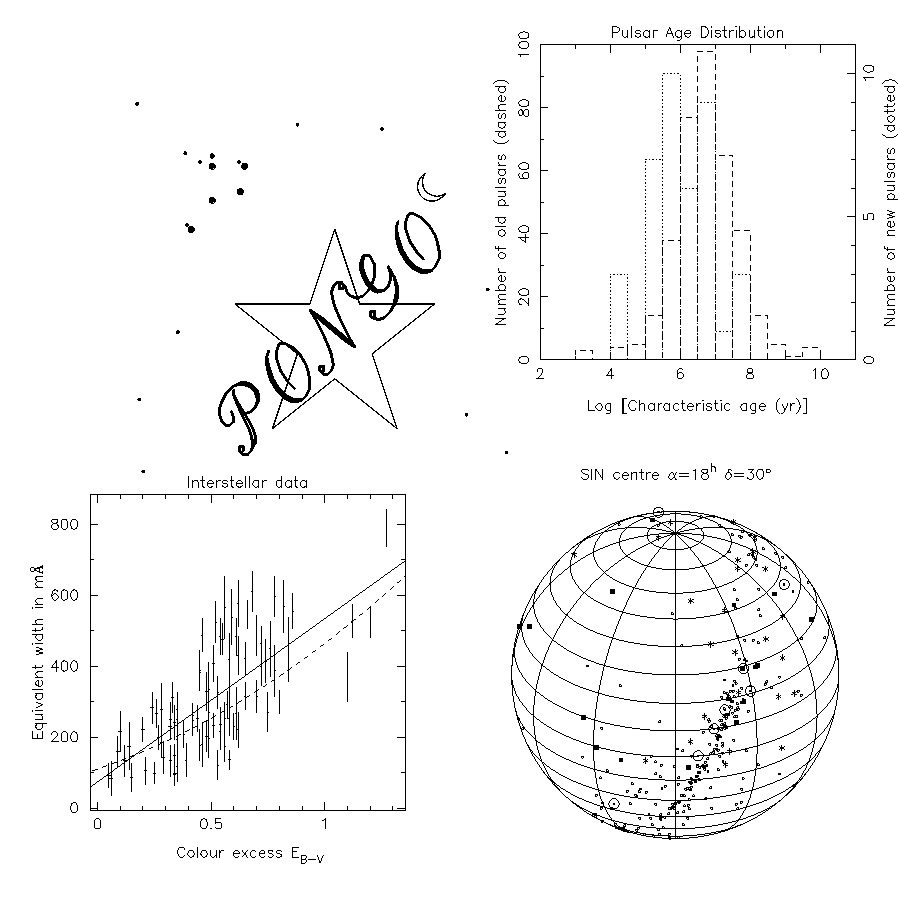
\includegraphics[width=100mm]{sun137_cover}
   \end{center}
   \vspace{5mm}

% ? Heading for abstract if used.
%   \vspace{10mm}
%   \begin{center}
%      {\Large\bf Abstract}
%   \end{center}
% ? End of heading for abstract.
\end{latexonly}

%  HTML documentation header.
%  ==========================
\begin{htmlonly}
   \xlabel{}
   \begin{rawhtml} <H1> \end{rawhtml}
      \stardoctitle
   \begin{rawhtml} </H1> \end{rawhtml}

% ? Add picture here if required.

   \htmladdimg{main.gif}

% ? End of picture

   \begin{rawhtml} <P> <I> \end{rawhtml}
   \stardoccategory \stardocnumber \\
   \stardocauthors \\
   \stardocdate
   \begin{rawhtml} </I> </P> <H3> \end{rawhtml}
      \htmladdnormallink{CCLRC}{http://www.cclrc.ac.uk} /
      \htmladdnormallink{Rutherford Appleton Laboratory}
                        {http://www.cclrc.ac.uk/ral} \\
      \htmladdnormallink{Particle Physics \& Astronomy Research Council}
                        {http://www.pparc.ac.uk} \\
   \begin{rawhtml} </H3> <H2> \end{rawhtml}
      \htmladdnormallink{Starlink Project}{http://www.starlink.ac.uk/}
   \begin{rawhtml} </H2> \end{rawhtml}
   \htmladdnormallink{\htmladdimg{source.gif} Retrieve hardcopy}
      {http://www.starlink.ac.uk/cgi-bin/hcserver?\stardocsource}\\

%  HTML document table of contents.
%  ================================
%  Add table of contents header and a navigation button to return to this
%  point in the document (this should always go before the abstract \section).
  \label{stardoccontents}
  \begin{rawhtml}
    <HR>
    <H2>Contents</H2>
  \end{rawhtml}
  \renewcommand{\latexonlytoc}[0]{}
  \htmladdtonavigation{\htmlref{\htmladdimg{contents_motif.gif}}
        {stardoccontents}}

% ? New section for abstract if used.
%  \section{\xlabel{abstract}Abstract}
% ? End of new section for abstract
\end{htmlonly}

% -----------------------------------------------------------------------------
% ? Document Abstract. (if used)
%  ==================
%\stardocabstract
% ? End of document abstract
% -----------------------------------------------------------------------------
% ? Latex document Table of Contents (if used).
%  ===========================================
 \cleardoublepage
 \begin{latexonly}
   \setlength{\parskip}{0mm}
   \latexonlytoc
   \setlength{\parskip}{\medskipamount}
   \markboth{\stardocname}{\stardocname}
 \end{latexonly}
% ? End of Latex document table of contents
% -----------------------------------------------------------------------------
\cleardoublepage
\renewcommand{\thepage}{\arabic{page}}
\setcounter{page}{1}
\newpage

\section{Introduction}

PONGO is a set of commands for interactively plotting data stored
in ordinary text files.
It is based around the \xref{PGPLOT (SUN/15)}{sun15}{} graphics
package.

Some highlights of PONGO are:

\begin{itemize}
\item Data are read from text files using a command (\cnam{\iref{READF}})
  that has:
  \begin{itemize}
  \item the ability to read files which contain character strings as well as
    numeric values;
  \item support for comment lines and column headings as an aid to remembering
    what the file contains;
  \item variable column delimiters, allowing \LaTeX\ and \TeX\
    format tables to be read;
  \item selective reading of the data;
  \item the ability to read in positions of Right Ascension and
    Declination in the format
    \begin{quote}
\begin{verbatim}
   HH:MM:SS.SSS   +DD:MM:SS.SSS
\end{verbatim}
    \end{quote}
  \end{itemize}
\item Plots of astronomical positional data can be made in one of several
  geometries (TAN, SIN, ARC, GLS, AITOFF, MERCATOR and STG).

\item Complicated mathematical manipulations can be performed on the data
  using  Fortran-like statements to define the required transformation.
\item Specialised extra data columns are provided, \ie \labcol\ for
  labels, \symcol\ for symbol numbers and \excol/\eycol\ for errors.
\item Many interactive cursor functions are provided.
\item Error ellipses can be drawn.
\item Vector plots can be drawn.
\item Simple statistical analysis of the data is available.
\item The data can be resampled.
\item Functions defined by Fortran-like statements can be drawn.
\end{itemize}

PONGO can used from both the Starlink/ICL and IRAF/CL
\footnote{at the time of writing IRAF support is no longer available
in a standard release} command languages and integrates with other Starlink
software packages.

Because the parameters PONGO uses for its commands are often similar
to the arguments of the equivalent PGPLOT subroutines, it is useful to
read the PGPLOT manual in conjunction with this user guide (if you are
not already familiar with PGPLOT).
In several cases the full descriptions of the parameters are given
only in the PGPLOT manual.

\section{Starlink/ICL or IRAF/CL?}
PONGO needs a command-language as a host environment and at present it
can be used from two that are generally available to astronomers; the
Starlink Interactive Command Language (ICL) and the IRAF Command
Language (CL).  You should use PONGO from which ever language is most
natural (\ie the one you or your colleagues are most familiar
with). There are no significant advantages to either system, however,
people intending to use IRAF/CL should note that most of this document
is slanted towards ICL usage (the original ``home'' of PONGO) and
should be prepared to consult the on-line help system, which should be
more IRAF specific.

Under IRAF/CL PONGO is available as the \verb+pongo+ package. From ICL
PONGO is available by just typing the \verb+pongo+ command.

\section{Tutorial Examples}
The following two sections show the same simple example. The first
uses the Starlink/ICL and the second the IRAF/CL command
languages.

\subsection{An ICL example}

In order to start PONGO you must first start ICL. This may be done by typing:
\begin{quote}
\begin{verbatim}
% pongo
\end{verbatim}
\end{quote}
at C-shell the prompt. Or alternatively by starting ICL then using the
\verb+pongo+ command.

In any PONGO session the first action is to open the plotting device.
This is done by typing\footnote{ If you have already used PONGO then
you should also issue the \cnam{\iref{RESETPONGO}} command immediately
after \cnam{\iref{BEGPLOT}}.}:
\begin{quote}
\begin{verbatim}
ICL> begplot xw
\end{verbatim}
\end{quote}

Where `\verb+xw+' should be replaced by the name of the plotting device you
are intending to use.  Note that once you have begun a PONGO session
with the \cnam{\iref{BEGPLOT}} command, the \verb+ICL>+ prompt changes
to \verb+PONGO>+. This is important because the only commands you can
use with success at the \verb+ICL>+ prompt are \cnam{\iref{BEGPLOT}}
and \cnam{\iref{DEVICE}}, all other commands should be typed at the
\verb+PONGO>+ prompt. The data may then be read using the
command \footnote{Note that the data file name is given as
\texttt{(TUTORIAL\_DATA)}, this uses an ICL variable which is set up
when PONGO is initialised}. Normally an `ordinary' file name would be
used \ie \texttt{spectrum.dat}. An ICL variable is used here as it is
not possible at this time to use an environment variable for accessing
formatted files. The actual file is
\texttt{\$PONGO\_EXAMPLES/tutorial.dat}:

\begin{quote}
\begin{verbatim}
PONGO> readf data=(TUTORIAL_DATA) xcol=1 ycol=3 all
\end{verbatim}
\end{quote}
Plotting limits are set up using the range of the data by the command:
\begin{quote}
\begin{verbatim}
PONGO> dlimits
\end{verbatim}
\end{quote}
Axes for the plot may be drawn using:
\begin{quote}
\begin{verbatim}
PONGO> boxframe
\end{verbatim}
\end{quote}
and finally the points may be plotted as asterisk-like symbols and the axes
labelled with:
\begin{quote}
\begin{verbatim}
PONGO> points 3
PONGO> label 'X axis' 'Y axis' 'Plot Title'
\end{verbatim}
\end{quote}
Note that the data values are remembered by PONGO and the plot you have
just created may be erased and recreated by typing:
\begin{quote}
\begin{verbatim}
PONGO> advance
PONGO> boxframe
PONGO> points
PONGO> label
\end{verbatim}
\end{quote}
To close a device and end a PONGO plot the command
\cnam{\iref{ENDPLOT}} should be used.  This is important if you are
going to switch to another set of applications such as
\xref{KAPPA}{sun95}{}, otherwise the plotting device characteristics
will be inaccessible to the second package.

\subsection{A CL example}

In order to start PONGO you must first start CL and load the
\verb+pongo+ package.

In any PONGO session the first action is to open the plotting device.
This is done by typing\footnote{ If you have already used PONGO then
you should also issue the \cnam{\iref{resetpongo}} command immediately
after \cnam{\iref{begplot}}.}:
\begin{quote}
\begin{verbatim}
po> begplot xw
\end{verbatim}
\end{quote}
Where `\verb+xw+' should be replaced by the name of the plotting device you
are intending to use. The data may then be read using the command:
\begin{quote}
\begin{verbatim}
po> readf data=pongoexamples$tutorial.dat xcol=1 ycol=3 all=yes
\end{verbatim}
\end{quote}
Plotting limits are set up using the range of the data by the command:
\begin{quote}
\begin{verbatim}
po> dlimits
\end{verbatim}
\end{quote}
Axes for the plot may be drawn using:
\begin{quote}
\begin{verbatim}
po> boxframe
\end{verbatim}
\end{quote}
and finally the points may be plotted as asterisk-like symbols and the axes
labelled with:
\begin{quote}
\begin{verbatim}
po> points 3
po> label "X axis" "Y axis" "Plot Title"
\end{verbatim}
\end{quote}
To close a device and end a PONGO plot the command:
\cnam{\iref{ENDPLOT}} should be used.

\section{Classified List of Commands}

This section presents a list of the available PONGO commands,
classified into several broad categories: commands which begin and end
a PONGO session, commands for manipulating data, commands which
control plotting, plotting commands, and commands which perform simple
statistics on the data.  Not all the commands given are individual
applications, many are synonyms (or scripts) for other applications
with specific parameters provided for convenience.  Detailed
descriptions of these commands are given in Appendix \ref{defn_sect}.
The parts of the command names outside parentheses define the minimum
abbreviation for that application (IRAF users should note that CL uses
its own abbreviations, which may not correspond to those below).


\subsection{Commands which begin and end PONGO}

\small
\begin {quote}
  \begin {description}
  \item [\iiref{BEGP(LOT)}{BEGPLOT}] -- Open a plotting device.
  \item [\iref{DEVICE}] -- Open a plotting device.
  \item [\iiref{ENDP(LOT)}{ENDPLOT}] -- Close down the current plotting device.
  \end {description}
\end {quote}
\normalsize


\subsection{Commands for plotting}

\small
\begin {quote}
  \begin {description}
  \item [\iiref{ADV(ANCE)}{ADVANCE}] -- Clear the graphics screen.
  \item [\iiref{ANN(OTATE)}{ANNOTATE}] -- Annotate the plotted data.
  \item [\iref{ARC}] -- Draw an arc of an ellipse.
  \item [\iref{BIN}] -- Plot a histogram using previously binned data.
  \item [\iiref{BOX(FRAME)}{BOXFRAME}] -- Draw a frame and axes on the plot.
  \item [\iiref{CONN(ECT)}{CONNECT}] -- Draw straight lines between the
    data points.
  \item [\iref{CURSE}] -- Use the cursor to get interactive input.
  \item [\iref{DRAWPOLY}] -- Draw a polygon.
  \item [\iref{DRAW}] -- Draw a line from the current pen position the specified
    point.
  \item [\iref{ELLIPSES}] -- Draw error ellipses.
  \item [\iref{ERASE}] -- Clear the graphics screen
  \item [\iref{ERRORBAR}] -- Draw error bars on the plotted data.
  \item [\iref{ERRX}] -- Draw symmetric error bars in the X direction.
  \item [\iref{ERRY}] -- Draw symmetric error bars in the Y direction.
  \item [\iref{GPOINTS}] -- Plot points or lines between the data.
  \item [\iref{GRID}] -- Draw a coordinate grid at specified intervals.
  \item [\iref{GT\_CIRCLE}] -- Draw a great circle between two points.
  \item [\iiref{HIST(OGRAM)}{HISTOGRAM}] -- Bin and plot a histogram of
    the data.
  \item [\iiref{LAB(EL)}{LABEL}] -- Draw the axis labels and title on
    the plot.
  \item [\iref{MARK}] -- Draw a point mark at the specified position.
  \item [\iref{MTEXT}] -- Draw a text string relative to the viewport.
  \item [\iiref{PLOTF(UN)}{PLOTFUN}] -- Plot a given function.
  \item [\iiref{PLOTH(IST)}{PLOTHIST}] -- Plot a histogram of the data.
  \item [\iiref{POI(NTS)}{POINTS}] -- Draw a point mark at each of the
    data points.
  \item [\iref{PRIM}] -- Perform primitive plotting functions.
  \item [\iref{PTEXT}] -- Draw a text string at the specified position and
    angle.
  \item [\iref{PVECT}] -- Draw proper motion vectors.
  \item [\iref{RADIATE}] -- Draw a line from the given point to the first NP
    data points.
  \item [\iiref{SIZE(PLOT)}{SIZEPLOT}] -- Draw point marks of differing
    sizes at each of the data points.
  \item [\iref{TEXT}] -- Draw a text string on the plot at the
    specified position.
  \item [\iref{VECT}] -- Draw vectors from each data point.
  \item [\iref{WTEXT}] -- Draw a text string on the plot.
  \item [\iref{XERR}] -- Draw symmetric error bars in the X direction.
  \item [\iref{YERR}] -- Draw symmetric error bars in the Y direction.
  \end {description}
\end {quote}
\normalsize


\subsection{Commands which control plotting}

\small
\begin {quote}
  \begin {description}
  \item [\iref{CHANGE}] -- Change plotting attributes.
  \item [\iref{CLEAR}] -- Clear plotting attributes.
  \item [\iiref{DLIM(ITS)}{DLIMITS}] -- Set the world coordinate limits
    using the data range.
  \item [\iiref{EXPA(ND)}{EXPAND}] -- Set the character height.
  \item [\iref{FILLSTY}] -- Change fill-style plotting attributes.
  \item [\iref{FONT}] -- Set the text font.
  \item [\iiref{INQ(UIRE)}{INQUIRE}] -- Display PONGO status information.
  \item [\iiref{LIM(ITS)}{LIMITS}] -- Set the world coordinate limits.
  \item [\iiref{LT(YPE)}{LTYPE}] -- Set the line style.
  \item [\iiref{LWE(IGHT)}{LWEIGHT}] -- Set the line width.
  \item [\iref{MOVE}] -- Set the current pen position.
  \item [\iiref{PALET(TE)}{PALETTE}] -- Change the plotting pen colours.
  \item [\iref{PAPER}] -- Change the size and aspect ratio of the plotting
    surface.
  \item [\iref{PEN}] -- Set the current pen.
  \item [\iiref{RESETP(ONGO)}{RESETPONGO}] -- Reset the state of PONGO.
  \item [\iref{SETPROJ}] -- Set the projection geometry.
  \item [\iiref{SHOWP(ONGO)}{SHOWPONGO}] -- Show the PONGO global parameters.
  \item [\iref{VIEWPORT}] -- Set the viewport for the current plotting device.
  \item [\iref{VPORT}] -- Set the viewport using normalised device coordinates.
  \item [\iref{VP\_BH}] -- Set the viewport to the bottom half of the plotting
    surface.
  \item [\iref{VP\_BL}] -- Set the viewport to the bottom-left quarter of the
    plotting surface.
  \item [\iref{VP\_BR}] -- Set the viewport to the bottom-right quarter of the
    plotting surface.
  \item [\iref{VP\_TH}] -- Set the viewport to the top half of the plotting
    surface.
  \item [\iref{VP\_TL}] -- Set the viewport to the top-left quarter of the
    plotting surface.
  \item [\iref{VP\_TR}] -- Set the viewport to the top-right quarter of the
    plotting surface.
  \item [\iref{VSIZE}] -- Set the viewport using its physical size in inches.
  \item [\iref{VSTAND}] -- Set the standard viewport.
  \item [\iref{WNAD}] -- Adjust the viewport so that the X and Y
    scales are the same.
  \item [\iref{WORLD}] -- Set the world coordinates for the plot.
  \end {description}
\end {quote}
\normalsize


\subsection{Commands for manipulating data}

\small
\begin {quote}
  \begin {description}
  \item [\iref{AVEDAT}] -- Average the data in the \xcol\ and \ycol\ areas.
  \item [\iref{CCMATH}] -- Perform inter-column maths.
  \item [\iref{CLOG}] -- Take the logarithm of a column.
  \item [\iref{DATA}] -- Specify the data file name.
  \item [\iref{DEGTOR}] -- Convert the specified data area from degrees to
    radians.
  \item [\iiref{EXC(OLUMN)}{EXCOLUMN}] -- Specify the column containing
    the X-axis error data.
  \item [\iiref{EYC(OLUMN)}{EYCOLUMN}] -- Specify the column containing
    the Y-axis error data.
  \item [\iiref{GETP(OINT)}{GETPOINT}] -- Retrieve information for a
    plotted data point.
  \item [\iiref{LABC(OLUMN)}{LABCOLUMN}] -- Specify the column used for
    data labels.
  \item [\iiref{PCOL(UMN)}{PCOLUMN}] -- Specify the column used for
    symbol codes.
  \item [\iref{PTINFO}] -- Get the coordinates of a specified data point.
  \item [\iiref{READ(F)}{READF}] -- Read from a formatted data file.
  \item [\iref{RTODEG}] -- Convert the specified data area from radians to
    degrees.
  \item [\iiref{SYMC(OLUMN)}{SYMCOLUMN}] -- Specify the column used for
    symbol codes.
  \item [\iiref{WRITE(I)}{WRITEI}] -- Write information to an output file.
  \item [\iiref{XC(OLUMN)}{XCOLUMN}] -- Specify the column containing the
    X-axis data.
  \item [\iiref{XLIN(EAR)}{XLINEAR}] -- Put 1\ldots N into the \xcol\ data
    area.
  \item [\iiref{XLOG(ARITHM)}{XLOGARITHM}] -- Take the logarithm of the
    X-axis data.
  \item [\iiref{XOFF(SET)}{XLOGARITHM}] -- Add a constant offset to the
    X-axis data.
  \item [\iref{XSCALE}] -- Multiply the values in the \xcol\ and \excol\ data areas
    by a constant.
  \item [\iiref{YC(OLUMN)}{YCOLUMN}] -- Specify the column containing the
    Y-axis data.
  \item [\iiref{YLIN(EAR)}{YLINEAR}] -- Put 1\ldots N into the YCOL data
    area.
  \item [\iiref{YLOG(ARITHM)}{YLOGARITHM}] -- Take the logarithm of the
    Y-axis data.
  \item [\iiref{YOFF(SET)}{YOFFSET}] -- Add a constant offset to the
    Y-axis data.
  \item [\iref{YSCALE}] -- Multiply the values in the \ycol\ and \eycol\ data areas
    by a constant.
  \item [\iiref{ZC(OLUMN)}{ZCOLUMN}] -- Specify the column containing the
    Z-axis data.
  \item [\iref{ZSCALE}] -- Multiply the values in the \zcol\ data area by a
    constant.
  \end {description}
\end {quote}
\normalsize


\subsection{Commands for performing simple statistics}

\small
\begin {quote}
  \begin {description}
  \item [\iiref{FITC(URVE)}{FITCURVE}] -- Fit a curve to the data.
  \item [\iiref{FITL(INE)}{FITLINE}] -- Fit a straight line to the data.
  \end {description}
\end {quote}
\normalsize


\section{Data File Formats} \label{data_sect}

The simplest form of input file for PONGO is a text file with the data
in columns separated by spaces, as in the file
\verb+$PONGO_EXAMPLES/tutorial.dat+ (or \verb+pongoexamples$tutorial.dat+).
However, PONGO allows a considerable level of fine control over the
data used for plotting from a particular file by providing for the use
of column delimiters, column labels and comments in data files.

\subsection{Column delimiters}

The default column delimiter is a space character, although the
\cnam{\iref{READF}} command does have the ability to use other
delimiters by setting the \pnam{DELIM} parameter.  It is possible for
more than one delimiter character to be used, \eg using \verb+&\+
would be a good way to read a table that was in \TeX\ format (\verb+&+
for a \LaTeX\ tabular format table).  A null string for the
\pnam{DELIM} parameter has the same effect as a single space.


\subsection{Column labels}

It is possible to give each column in a file a symbolic name that can be used
to reference the column when reading the file and can be automatically
transferred to the appropriate axis label on the plot.
To do this, the first line of the file should be of the form:
\begin{quote}
\begin{verbatim}
!$label 1$label 2$label 3$
\end{verbatim}
\end{quote}
where there are as many labels, each delimited by a \verb+$+, as there are
columns.
Care should be taken to ensure that there is no leading white space in the
column labels, although it is permissible for the column labels to contain
white space elsewhere.
Any padding that is required to make the column labels line up with the data
columns should be achieved with multiple dollar signs,
\eg:
\begin{quote}
\begin{verbatim}
!$RA$$$$Declination$
\end{verbatim}
\end{quote}
When specifying the column on the command line, \eg \cnam{YCOL Dec},
it is permissible to abbreviate the string to a minimum match.
However, {\em the match is case-sensitive.}


\subsection{Comments}

Comments may be placed in the data file by prefixing the line with one
of the standard comment characters.  There are two comment characters
allowed in the data file, specified by the parameters \pnam{HARDCOMM}
and \pnam{SOFTCOM} for the command \cnam{\iref{READF}}.  These comment
characters must occur in the first column of a line to be recognised
as comment characters.  The main purpose of comment characters is to
document data files and to comment out unwanted lines of data.  The
existence of two comment characters provides the ability to
selectively read data subsets from files.  Blank lines are ignored in
data files.

Although not recommended practice, the documentation of data files can
be done without the use of comment characters: because PONGO will
reject any line in which the required numerical column cannot be
interpreted as a valid number, it does not matter whether a comment
character is put at the start of the line or not.


\subsection{Astronomical coordinates}

It is possible to read data stored in an astronomical coordinate
format (\ie \verb+HH:MM:SS.SSS+ and \verb+DD:MM:SS.SSS+) into PONGO.
The data is stored internally in {\em radians}: in this conversion any data
read into \xcol\ is assumed to be a Right Ascension (\ie of the first
form above) and any data read into \ycol\ is assumed to be a
Declination (\ie of the second form above).

The \cnam{\iref{BOXFRAME}} command can label axes using a
\verb+HH MM SS.S+ and \verb+DD MM SS.S+ format providing the data and frame limits
are specified in radians.

\section{Internal Data Areas}

There are seven internal data areas into which data may be read.
These are as follows:

\begin{quote}
\begin{description}
\item [\xcol] -- This area is principally intended to hold X-axis
data.  However, when using the command \cnam{\iref{PLOTHIST} H}, this
area is intended to hold the data before they are binned to draw the
histogram.

When using the command \cnam{\iref{ERRORBAR} X} with the symmetric
option turned off, this area contains the position of one of the ends
of the error bar.

\item [\ycol] -- This area is intended to hold Y-axis data.

When using the command \cnam{\iref{ERRORBAR} Y} with the symmetric
option turned off, this area contains the position of one of the ends
of the error bar.

\item [\excol] -- This area is principally intended to hold errors for the
X-axis data values.
These errors are generally assumed to be symmetric about the data point
by the command \cnam{\iref{ERRORBAR}}, but with the symmetric option turned off
\excol\ holds the position of the opposite end of the error bar to
\xcol.

The \excol\ area is assumed to contain the standard error of the \xcol\ data by
the command \cnam{\iref{ELLIPSES}}.

The \excol\ area is also used to hold the X-axis component of the
vector offset from the data point by the command \cnam{\iref{VECT}},
and the proper motion in Right Ascension by the command
\cnam{\iref{PVECT}}.

When using the command \cnam{\iref{ARC}}, the \excol\ data are assumed
to contain the magnitude of the semi-major axis of the ellipse.

The command \cnam{\iref{AVEDAT}} will write the standard deviation of
the average it calculated for each bin into the \excol\ data area.

\item [\eycol] -- Similar to \excol, but applying to the Y-axis data values.

The \eycol\ area is used to hold the Y-axis component of the vector
offset from the data point by the command \cnam{\iref{VECT}}, and the
proper motion in Declination by the command \cnam{\iref{PVECT}}.

When using the command \cnam{\iref{ARC}}, the \eycol\ data are assumed
to contain the magnitude of the semi-minor axis of the ellipse.

\item [\zcol] -- PONGO does not have the ability to draw three
dimensional plots.
As a result, the \zcol\ data area does not contain Z-axis data in the
conventional sense.
However, there are a number of commands that use the values stored in the
\zcol\ area.

The command \cnam{\iref{SIZEPLOT}} uses the values stored in \zcol\ to
scale the size of the marker symbols plotted for each data point.

The commands \cnam{\iref{VECT}} and \cnam{\iref{PVECT}} can optionally
use the values in \zcol\ to scale the length of the vectors they draw.

The command \cnam{\iref{ELLIPSES}} assumes that \zcol\ contains the
values of the normalised covariances between the X- and Y-axis errors.

\item [\labcol] This area is used for storing a character string
associated with each of the data points.  The strings may be plotted
interactively using the \cnam{\iref{ANNOTATE}} or \cnam{\iref{CURSE}}
commands.

\item [\symcol] This area is used to store a PGPLOT symbol number (an
\verb+INTEGER+) associated with each of the data points.

% Note that this symbol number is not restricted to the 32 specified as
% markers in the PGPLOT manual, any of the Hershey character numbers can
% be used as well.
\end{description}
\end{quote}


\section{Projections} \label{proj_sect}

PONGO is capable of plotting astronomical coordinate data in one of several
`projections' or, more strictly, in one of several geometries (not all of the
`projections' are true projections onto a plane, but are geometries that have
other properties -- \eg the equal area property where areas are preserved in
the transformation from the celestial sphere to a two dimensional plot).
{\em Table \ref{proj_tab}} lists the geometries available in PONGO.

All the main point plotting commands will work in any of the available
geometries.
They assume that the data in the \xcol\ and \ycol\ areas are stored internally
in radians and refer to the longitude and latitude respectively of the point to
be plotted.
Where the position values are to be entered on the command line, the latitude
and longitude are normally given in degrees.

In addition to the point plotting commands, there are also three commands whose
only use is when plotting in a particular projection type:

\begin {quote}
\begin{description}
\item [\iref{GRID}] -- Plot a coordinate grid in the current projection.
                       The default parameters of this command are to draw a
                       grid over the whole sky with a longitude line every 30
                       degrees and a latitude line every 10 degrees.
\item [\iref{GT\_CIRCLE}] -- Draw a great circle between two specified points
                             on the celestial sphere.
\item [\iref{PVECT}] -- Draw proper motion vectors from each plotted point as
                        small great circle arcs.
\end{description}
\end {quote}

\begin{table}[t]
\centering
\begin{tabular}{|l|p{0.6\textwidth}|}
\hline
Projection & Description \\
\hline
NONE     & No projection is used. \\
AITOFF   & The Aitoff projection (has an equal area property). \\
ARC      & Move an equal distance on the tangent plane as a great circle on the
celestial sphere. \\
GLS      & Right Ascension intervals are multiplied by $\cos\delta$ (has an
equal area property). \\
MERCATOR & The Mercator projection. \\
SIN      & Drop a perpendicular onto the tangent plane. \\
STG      & The Stereographic projection. \\
TAN      & Projection onto the tangent plane through the centre of the
celestial sphere. \\
\hline
\end{tabular}
\caption{Projection geometries available in PONGO} \label{proj_tab}
\end{table}


\section{Creating Complex Plots}

Repeating complex sequences of PONGO commands by hand can become
boring and is likely to lead to many mistakes (particularly on those
occasions when you want to create a hardcopy and cannot even see the
current state). The way to get around these problems is to use the
abilities of the ICL or CL command languages to create {\em
procedures}.

The following two sections show extremely simple examples of how to
start doing this in both languages. To get further you'll need to
consult the appropriate documentation, \xref{SG/5}{sg5}{} in the case
of ICL and the ``{\em CL Programmer's Manual}'' and
``{\em An Introductory User's Guide to IRAF Scripts}'' for CL.

\subsection{A simple ICL procedure}

A simple procedure that reproduces the tutorial example looks like:
\begin{quote}
\begin{verbatim}
proc icltest file
   begplot xw
   readf data=(file) xcol=1 ycol=3 all reset
   dlimits
   boxframe
   points 3
   label 'X axis' 'Y axis' 'PLOT TITLE'
   endplot
endproc
\end{verbatim}
\end{quote}
If you enter this text into a file say called \verb+icltest.icl+ and use
the following commands from ICL:
\begin{quote}
\begin{verbatim}
ICL > load icltest
ICL > icltest (TUTORIAL_DATA)
\end{verbatim}
\end{quote}
The data from the tutorial example will be plotted as before. One
immediate advantage of this method is that we can now plot data from
columns 1 and 3 of any file.

If the contents of the procedure are wrong or need a slight
modification then you can edit the procedure from ICL. Try the command:
\begin{quote}
\begin{verbatim}
ICL > edit icltest
\end{verbatim}
\end{quote}
This puts you into an editor and you can modify the procedure. (If you
haven't set an environment variable EDITOR or used the ICL command
\verb+set editor+, you'll find yourself in \verb+vi+. To exit from this
type the command \verb+:q+ and now use the \verb+set editor+
command.) If you made a modification to the procedure this can be
viewed using the command:
\begin{quote}
\begin{verbatim}
ICL > list icltest
\end{verbatim}
\end{quote}
All the currently available procedures are shown using the command:
\begin{quote}
\begin{verbatim}
ICL > procs
\end{verbatim}
\end{quote}
If you do modify a procedure from ICL use the:
\begin{quote}
\begin{verbatim}
ICL > save icltest
\end{verbatim}
\end{quote}
command to write out your changes (you should use the name of your procedure
instead of \verb+icltest+).

\subsection{A simple CL procedure}

A simple CL procedure that reproduces the tutorial example looks like:
\begin{quote}
\begin{verbatim}
procedure cltest (datafile)
string datafile
begin
   begplot xw
   readf (data=datafile, xcol=1, ycol=3, all=yes, mode=h )
   dlimits
   boxframe
   points 3
   label ("X axis", "Y axis", "PLOT TITLE")
   endplot
end
\end{verbatim}
\end{quote}
If you enter this text into a file say called \verb+cltest.cl+ and use
the following commands from CL.
\begin{quote}
\begin{verbatim}
po> task cltest = cltest.cl
po> cltest pongoexamples$tutorial.dat
\end{verbatim}
\end{quote}
The data from the tutorial example will be plotted as before. One
immediate advantange of this method is that we can now plot data from
columns 1 and 3 of any file.

Another way in which you can create CL scripts is to use the
\verb+mkscript+ command.

\subsection{Example procedures} \label{exam_sect}

These examples are intended to show some of the features of PONGO and
also provide examples of complex procedures for both the ICL and CL
command-languages. All these procedures can be
found in the directories \verb+$PONGO_EXAMPLES+  and
\verb+pongoexamples$+ respectively. ICL examples have file extensions
\verb+.icl+ and CL examples \verb+.cl+.

The ICL procedures will prompt for a graphics device and should be
invoked from the \verb+ICL>+ prompt using the ICL command \verb+load+, \eg:
\begin {quote}
\begin{verbatim}
ICL> load $PONGO_EXAMPLES/ppdotdiag
\end{verbatim}
\end {quote}
and their execution can be followed if the ICL command \verb+set trace+ has
previously been executed.

The CL procedures are defined as tasks by the \verb+pongo+ command and
can be run by just typing their name \ie:
\begin{quote}
\begin{verbatim}
po> ppdotdiag
\end{verbatim}
\end{quote}

Note that some of the examples involve the colour representation of lines,
which may be difficult to see on a greyscale device (\eg on a monochrome
Postscript device).
It is recommended that a colour image display device is used to run the
example procedures.

\newpage

\subsubsection{Spectrum}

This procedure produces {\em Figure \ref{SPECTRUM}}, a plot of a
low resolution
IUE spectrum extracted by \xref{IUEDR (SUN/37)}{sun37}{} and written using the
IUEDR command \verb+OUTSPEC SPECTYPE=2+.
The output file was subsequently edited to make the file label lines PONGO
comments and to add a line of PONGO column labels (see \S\ref{data_sect})
at the beginning of the file.
IUEDR indicates bad or missing data in an output spectrum by attributing zero
fluxes to the affected wavelength samples.
These can be detected and discarded using the \pnam{SELCOND} parameter of
the \cnam{\iref{READF}} command: \eg

\begin{quote}
\begin{verbatim}
PONGO> readf (SWP_DATA) selcond="Flux > 0.0" noall
\end{verbatim}
\end{quote}

In this example PONGO draws a polyline across all missing data flagged by
IUEDR.

\halfpfig{sun137_fig1}{SPECTRUM}{spectrum.gif}{6in}
\newpage


\subsubsection{Errors}

The procedure \verb+ERRORS+ was used to plot {\em Figure
\ref{ERRORS}}.  This example demonstrates plotting simple error
bars using PONGO (the \cnam{\iref{ERRORBAR}} command) and also
performing simple statistics on the data (the \cnam{\iref{FITLINE}}
and \cnam{\iref{FITCURVE}} commands).  Note that a summary of the
statistics is reported for each fit to the data.

\halfpfig{sun137_fig2}{ERRORS}{errors.gif}{6in}
\newpage


\subsubsection{Histogram}

The procedure \verb+HISTOGRAM+ (\verb+histogramtest+ from CL) was used to
plot {\em Figure \ref{HISTOGRAM}}, which illustrates the plotting
of histograms with PONGO (the \cnam{\iref{PLOTHIST}} command).  This
procedure also illustrates how the drawing of the box around the plot
can be controlled using the \cnam{\iref{BOXFRAME}} command.

\halfpfig{sun137_fig3}{HISTOGRAM}{histogram.gif}{6in}
\newpage


\subsubsection{Ppdotdiag}

This procedure produces {\em Figure \ref{PPDOTDIAG}}, a period
versus period derivative diagram for pulsars.  Note the use of a
column within the data file to set the symbol number of each plotted
point, and the use of the \verb+PONGO_NDATA+ global parameter for
making a title containing the number of points that have been read in
(in CL this uses the output parameter \verb+readf.ndata+)

\halfpfig{sun137_fig4}{PPDOTDIAG}{ppdotdiag.gif}{6in}
\newpage


\subsubsection{Ellipses}

The procedure \verb+ELLIPSES+ (\verb+ellipsetest+ from CL) was used to plot
{\em Figure \ref{ELLIPSES}}, which illustrates the use of the
\cnam{\iref{ELLIPSES}} command for plotting error ellipses.

\halfpfig{sun137_fig5}{ELLIPSES}{ellipses.gif}{6.5in}
\newpage


\subsubsection{Projections}

This procedure illustrates some of the different `geometries'
available in PONGO.  It plots four different views of the distribution
of a selection of the known pulsars in Right Ascension and Declination
to produce {\em Figure \ref{PROJECTIONS}}.

\halfpfig{sun137_fig6}{PROJECTIONS}{projections.gif}{6in}
\newpage

\subsubsection{Radec}

This procedure shows how the \cnam{\iref{BOXFRAME}} command can be
used to draw labels in \verb+HH MM SS.S+ \& \verb+DD MM SS.S+
format.
The output from it is shown in {\em Figure \ref{RADEC}}.
The objects are some of the pulsars from
{\em Figures \ref{PROJECTIONS}} and {\em \ref{PPDOTDIAG}}.
\halfpfig{sun137_fig7}{RADEC}{radec.gif}{6in}
\newpage

\subsubsection{Vector}
This procedure shows the \cnam{\iref{VECT}} and \cnam{\iref{PVECT}}
commands being used to plot the proper motion vectors of a set of
bright stars. The stars are selected to have proper motions in
RA greater than 0.5 arcseconds and the distances shown correspond to
100000 years of travel.

\halfpfig{sun137_fig9}{VECTOR}{vector.gif}{6in}
\newpage

\subsubsection{Interactive}

After executing the examples it is a good idea to gain some
experience with the \cnam{\iref{CURSE}} application.  This can be done
using the procedure \verb+INTERACTIVE+.  The procedure will plot a
graph and then invoke the \cnam{\iref{CURSE}} application, resulting
in the following instructions being printed on the screen:
\begin{quote}
\begin{verbatim}
CURSE cursor options:
   Q - Quit.
   D - Draw to the cursor position.
   E - Expand the plotting limits.
   G - Calculate the gradient.
   L - Label the plot.
   M - Mark a point.
   O - Left justified annotation.
   P - Right justified annotation.
   S - Shrink the plotting limits.
   V - Move to the cursor position.
   X - Get the cursor position.
   Z - Zoom the plotting limits.
\end{verbatim}
\end{quote}
where the letter signifies the key that is to be pressed on the keyboard to
achieve the desired effect.

If you have examined the example file for \verb+INTERACTIVE+ you will
have seen that a label has been read in for each of the data points.
It is now possible for you to use these labels by moving the cursor close to a
plotted point and pressing \verb+O+ or \verb+P+.
When you do this, a label for the point nearest the cursor will be written at
the cursor position.
Do this for several points and then press \verb+Q+ to exit from the
\cnam{\iref{CURSE}} command.
PONGO will have remembered the particular labelling that that you have
performed and will then use the command \cnam{\iref{WRITEI} LABLST=YES} to
write the PONGO commands required to recreate these labels to a
specified file.  (You can use the procedure \verb+INTERACTIVE+ to
explore the other functions of the \cnam{\iref{CURSE}} application.)

The \zcol\ area has been filled with the distances to each of the
pulsars.
These values can be used to plot points whose sizes are inversely proportional
to distance (\ie the closer pulsars are larger) by first taking the reciprocal
of the \zcol\ area with the \cnam{\iref{CCMATH}} command:
\begin{quote}
\begin{verbatim}
PONGO> CCMATH Z=1/(Z+0.1)
\end{verbatim}
\end{quote}
and then the points plotted with the command:
\begin{quote}
\begin{verbatim}
PONGO> SIZEPLOT
\end{verbatim}
\end{quote}
Note here that a small positive value has been added to the distance data
(\ie {\tt Z+0.1}) to avoid very large symbols for nearby pulsars.


\newpage
\subsubsection{AGI}

This example illustrates the interaction between the \xref{KAPPA
package (SUN/95)}{sun95}{} and PONGO via the \xref{AGI graphics
database}{sun48}{}.  Here, the image display has been done using the
\xref{KAPPA \cnam{DISPLAY}}{sun95}{DISPLAY} command and PONGO has been
used for all the line drawing (note this example is not available
under CL).

\halfpfig{sun137_fig8}{AGI}{agi.gif}{7in}
\newpage


\section{Using PONGO with other Starlink Applications}

Using graphics between different applications packages is often difficult
because once one package has finished plotting and completed execution all
information concerning the contents of the plot is lost.
This problem may be overcome by storing relevant graphical information for the
plot (\eg the graphics device, the size and position of the plot on the display
surface, the coordinate limits of the data) in a file and providing facilities
to store and retrieve the information in this database.
This allows different applications to be used to display images, draw contours
and  annotate, for example, on the same plot without each application losing
access to the plot dimensions.
One such facility is provided by Starlink and is called
\xref{AGI -- Applications Graphics Interface (SUN/48)}{sun48}{}.
As its name implies, this facility provides a means by which any application
can store plotting information for later use and retrieve plotting information
stored by previous applications.
To use AGI to good effect requires familiarity with some nomenclature.

AGI divides the plotting surface up into {\bf pictures}, where a picture
represents a rectangular area on the display surface.
AGI stores coordinate information for each picture it creates on a graphics
device in its database.
AGI pictures are independent of the graphics package used to plot the data
(where supported; \ie SGS, IDI or PGPLOT), but they do depend explicitly upon
the graphics device used to plot the data.
AGI stores each picture in its database, grouped by the graphics device (or
{\bf workstation} in Starlink graphics terminology) upon which the picture was
created, and each is stored sequentially in the order in which they were
created.
AGI pictures are given a name which indicates their use:
a {\bf BASE} picture refers to the whole plotting surface and the name is
reserved only for this use;
a {\bf FRAME} picture refers to a picture which contains other pictures;
and a {\bf DATA} picture refers to a picture which contains a plot of the data.
AGI also stores a label for each picture: a short character string which
can be used by an application to uniquely identify a picture.
Finally, AGI can store a one-line comment for each picture in the database to
describe its use.

PONGO uses the definitions of {\bf world coordinates}, {\bf window},
{\bf device coordinates} and {\bf viewport} used by the
\xref{PGPLOT graphics package (SUN/15)}{sun15}{} upon which it is based.
Here, a PONGO plot represents a window of given size in the data or world
coordinates the you're working in.
The data are plotted within these world coordinate limits in a rectangular
area of the workstation surface.
This area is called the viewport and its size and shape are defined in terms of
the device coordinates.
The data are plotted exactly within this viewport and so plot annotation and
labelling will normally extend beyond the viewport limits.
AGI pictures refer directly to PONGO viewports.
Clearly, not all viewports used by PONGO will be associated with data windows
and refer to plotted data; many will just define regions of the workstation
surface in which further viewports will be defined.
These viewports are directly analogous to the AGI FRAME pictures and are
stored as such by AGI.
Those viewports which are used for plotting data within are directly analogous
to AGI DATA pictures and again are stored as such by AGI.

By default, when \cnam{\iref{BEGPLOT}} (or \cnam{\iref{DEVICE}}) is used to
begin a new PONGO plotting session; \eg:
\begin{quote}
\begin{verbatim}
ICL> begplot xw
\end{verbatim}
\end{quote}
PONGO will open the device and use the AGI BASE picture for that device, unless
there is a more recent picture.
In the case of a more recent picture, a FRAME picture will be created with the
dimensions of the picture current on entry.
In either case, the workstation will also be cleared.
When a PONGO plot ends, using \cnam{\iref{ENDPLOT}}, the AGI picture current on entry
is again made current.

There are two further modes in which a PONGO plot may be begun: assert
that PONGO use the BASE picture for plotting (\cnam{\iref{BEGPLOT} ACTION=B});
and assert that PONGO use the last DATA picture in the
current FRAME, without clearing the graphics device (\cnam{\iref{BEGPLOT}
OVERLAY NOCLEAR}).  Specifying \cnam{\iref{BEGPLOT} ACTION=B} forces PONGO to
make the AGI BASE picture current on entry; \ie if you specifically
want to use the whole display surface for plotting.
Using \cnam{\iref{BEGPLOT} OVERLAY=YES CLEAR=NO} allows plotting with other
applications packages in a coordinated way.  Here, PONGO will search
for the last DATA picture in the AGI database and use the associated
coordinates to define the PGPLOT viewport.  The workstation will not
be cleared on entry.  This means that anything plotted with PONGO will
be on the same axes and to the same scale as the existing plot.

As an example, PONGO can be used to annotate images displayed using
\xref{KAPPA}{sun95}{}.  First, KAPPA will be used to set the image
display device and to clear the AGI database for the device (\ie a
tidy start):
\begin{quote}
\begin{verbatim}
ICL> kappa
ICL> idset xw
ICL> idclear
\end{verbatim}
\end{quote}
It is necessary to first define the viewport the image is to be plotted within
using PONGO in order to assure that there is enough room around the image for
the annotation (remember, the annotation of PONGO graphs normally lies outside
the viewport):
\begin{quote}
\begin{verbatim}
ICL> pongo
ICL> begplot xw
PONGO> vstand
PONGO> endplot
\end{verbatim}
\end{quote}
Then use \xref{KAPPA}{sun95}{DISPLAY} to display the
image\footnote{The image actually displayed is defined, in this case,
by the ICL variable \texttt{DOR\_DATA}. This is set to the value
\texttt{\$PONGO\_EXAMPLES/dor} when PONGO is started.}:
\begin{quote}
\begin{verbatim}
ICL> picdata
ICL> display (DOR_DATA) mode=perc percentiles=[3,99.9]
ICL> lutheat
\end{verbatim}
\end{quote}
Here, \xref{KAPPA PICDATA}{sun95}{PICDATA} is used to select the last
defined AGI DATA picture, which is a DATA picture created by PONGO
with enough space around it to annotate the plot. You could also use
\xref{KAPPA PICLIST}{sun95}{PICLIST} which shows a table of all the
pictures in the AGI database.  These include the BASE picture,
referring to the entire plotting surface of the graphics device;
the PONGO FRAME picture, defined on entry and again referring to the
entire plotting surface; and finally the PONGO DATA picture, referring
the area of the plotting surface within which the image is displayed.

Now PONGO may be used to annotate the plot:
\begin{quote}
\begin{verbatim}
ICL> begplot xw overlay noclear
PONGO> boxframe bcinst bcinst
PONGO> label "X-axis pixel" "Y-axis pixel" "KAPPA image"
PONGO> endplot
\end{verbatim}
\end{quote}
The image has been displayed by \xref{KAPPA}{sun95}{} and then the
axes drawn and annotated using PONGO.  In this case, the annotation
represents the pixel number in each of the axes of the image.  A more
detailed example of the interaction between \xref{KAPPA}{sun95}{} and
PONGO, via \xref{AGI}{sun48}{}, is provided in \S\ref{exam_sect}.

\section{Panic Section}

\subsection{Getting help in ICL}

When in ICL, on-line help on PONGO may be examined using the command:
\begin{quote}
\begin{verbatim}
ICL> help pongo
\end{verbatim}
\end{quote}
This will provide a brief description of the package and how to begin and end a
PONGO plotting session.
Once the PONGO commands have been made available within ICL, \ie by typing
\begin{quote}
\begin{verbatim}
%  pongo
\end{verbatim}
\end{quote}
at the C-shell prompt or:
\begin{quote}
\begin{verbatim}
ICL> pongo
\end{verbatim}
\end{quote}
at the \verb+ICL>+ prompt, on-line help on any PONGO command may be examined
using the command:
\begin{quote}
\begin{verbatim}
ICL> help <pongo command>
\end{verbatim}
\end{quote}
The command:
\begin{quote}
\begin{verbatim}
ICL> help pongo
\end{verbatim}
\end{quote}
will produce a brief introduction to PONGO, and the command:
\begin{quote}
\begin{verbatim}
ICL> help introduction
\end{verbatim}
\end{quote}
will produce a more detailed introduction to PONGO and how to get
started.  These help commands are also available at the \verb+PONGO>+
prompt.  A classified list of PONGO applications (\cnam{HELP
CLASSIFIED}) is provided within the help system and help is also
provided on running the PONGO examples (\cnam{HELP EXAMPLES}).

If difficulties are encountered with PONGO and the on-line help system
does not reveal the cause, it is recommended that the relevant
sections of this document are read, or re-read.  It may be that this
document does not provide enough detail concerning the behaviour of
the PGPLOT graphics package: for detailed information regarding
PGPLOT, the PGPLOT manual should be consulted (available as a
Miscellaneous User Document, MUD, at all Starlink sites).  As a last
resort, the problem may be regarded as a software bug and reported to
the Starlink Software support mailing list (starlink@jiscmail.ac.uk).


\subsection{\cnam{BEGPLOT} or \cnam{DEVICE} does not work in ICL}

If the error message:
\begin{quote}
\begin{verbatim}
TOOFEWPARS   Not enough procedure parameters
\end{verbatim}
\end{quote}
is returned after the \cnam{\iref{BEGPLOT}} or \cnam{\iref{ENDPLOT}}
commands have been invoked, the reason is that another application
package or ICL procedure has switched parameter checking on within ICL
\xref{(SG/5)}{sg5}{}.  The problem is simply overcome by typing the command:
\begin{quote}
\begin{verbatim}
ICL> set nocheckpars
\end{verbatim}
\end{quote}
The PONGO commands will then work correctly.

\subsection{\cnam{READF} cannot find a column label}

If a column label is used with the \cnam{\iref{READF}} command instead
of the column number (see \S\ref{data_sect}) and \cnam{\iref{READF}}
fails, \eg:
\begin{quote}
\begin{verbatim}
PONGO> readf myfile.dat xcol=1 ycol=3 zcol="ZCOL"
File: /disk/scratch/jbloggs/plots/myfile.dat
XCOL - 1 is column number 1.
YCOL - 3 is column number 3.
!! ZCOL incorrectly specified as ZCOL.
!  READF: Data could not be read.
\end{verbatim}
\end{quote}
then either the data file does not have column labels or the incorrect
column label has been used.
It is of particular significance here that the column labels are {\em
case-sensitive}.
In fact, JBLOGGS found that the column label for his \zcol\ data was
\pnam{Zcol}:
\begin{quote}
\begin{verbatim}
PONGO> readf myfile.dat xcol=1 ycol=3 zcol="Zcol"
File: /disk/scratch/jbloggs/plots/myfile.dat
XCOL - 1 is column number 1.
YCOL - 3 is column number 3.
ZCOL - Zcol is column number 5.
EXCOL - 0 is column number 0.
EYCOL - 0 is column number 0.
LABCOL - 0 is column number 0.
SYMCOL - 0 is column number 0.
42 data points read.
PONGO>
\end{verbatim}
\end{quote}


\subsection{Strange behaviour of \cnam{DLIMITS}}

If PONGO does not seem to be doing something correctly, it is often
because there are unwanted data in the error columns.  This can come
about when a file that does not contain errors is read (the
appropriate parameters to \cnam{\iref{READF}} have been set to zero),
following one where there have been errors.
Here, it should be noted that setting a column parameter in
\cnam{\iref{READF}} to zero means that no data will be read from the
file into that particular area, it does not clear the data values.
This is a feature rather than a bug, because it allows X and Y data from two
different files to be plotted together, as long as each file contains the same
number of points (the number of points read from the second file is
assumed to be the number required).
Although advantageous, it is possible for the internal data areas to get into a
mess with this arrangement.
If this seems to have happened then the command:
\begin{quote}
\begin{verbatim}
PONGO> clear data
\end{verbatim}
\end{quote}
should be used to clear all the data areas.


\subsection{Error messages from \cnam{SHOWPONGO} in ICL}

The commands \cnam{\iref{SHOWPONGO}} may sometimes deliver the error messages
\begin{quote}
\begin{verbatim}
!! Object 'PONGO_<param>' not found.
!! DAT_FIND: Error finding a named component in an HDS structure.
\end{verbatim}
\end{quote}
when invoked (\verb+<param>+ refers to a PONGO parameter name in this
context).
The reason is simply that no global parameter of that name currently exists.
This can either be because PONGO has not been used before (or not a lot),
or because the ADAM global parameter file (\verb+$HOME/adam/GLOBAL.sdf+) has
been deleted since the last PONGO session.
Although the error messages look alarming, they are harmless.
To stop these error messages being output, the command \cnam{\iref{RESETPONGO}}
should be executed.
This command will assign a default value to each of the PONGO global parameters
except \pnam{PONGO\_DATA}, the data file name used by \cnam{\iref{READF}}, and
\cnam{\iref{SHOWPONGO}} will be subsequently more informative.


\subsection{AGI problems}

The \xref{AGI}{sun48}{} database is normally kept in a separate
\xref{HDS file}{sun95}{} \xref{(SG/4)}{sg4}{} for each machine in your
\verb+$HOME+ directory.  The command \cnam{\iref{BEGPLOT}} opens the
AGI database and reads database information relevant to the graphics
device being used.  During a PONGO plotting session, the database file
is held open to update the database as the plotting session proceeds.
At the end of plotting, when \cnam{\iref{ENDPLOT}} is executed, the
update of the database is completed and the database file is closed.
If another non-PONGO application which uses AGI is run before the
current PONGO plotting session has been ended (\ie using
\cnam{\iref{ENDPLOT}}), it will be unable to access the AGI database and will
subsequently fail.  In the event of this happening, using the PONGO
\cnam{\iref{ENDPLOT}} command will restore the correct behaviour of the
non-PONGO application.

What is more important, in order to use AGI successfully, is the use
of \cnam{\iref{ENDPLOT}} before exiting ICL or CL.  Because PONGO keeps the
AGI database file open throughout a plotting session it is possible to
exit ICL or CL without having first executed \cnam{\iref{ENDPLOT}}.  If this
is done, it is likely that the AGI database will not have been fully
updated before being closed, with the result that the next time AGI is
used it will behave inconsistently.  PONGO crashing during a plotting
session (hopefully, a rare event) can also result in a corrupted AGI
database.  There is no solution to this problem other than to delete
the database file and start again.  The AGI database files are kept in
the directory \verb+$HOME+ and have names of the form
\verb+agi_<machine>.sdf+, where \verb+<machine>+ is the name of the
machine on which AGI is being used.  This file may be deleted at any
time before a \cnam{BEGPLOT} command or after an \cnam{ENDPLOT} command.
The \cnam{\iref{BEGPLOT}} command may then be used to begin a new PONGO plot,
creating a new AGI database as a result.


\subsection{RESET peculiarity (ICL only)}

When using the ADAM parameter system \xref{(SG/4)}{sg4}{} \pnam{RESET}
qualifier to set parameters back to their default values (this
facility would be particularly useful for \cnam{\iref{BOXFRAME}}, for
example), there will be no effect on parameters which get their values
from global parameters. Use the \cnam{\iref{RESETPONGO}} command to
reset global parameters, or alternatively (somewhat drastically)
delete the \verb+GLOBAL.sdf+ file.

\subsection{Plotting large numbers of positions}
PONGO can store $5000$ positions at any time. This can very
occasionally cause problems for specific types of use. One way in
which you can actually plot more positions than this, is by reading in
the data in chunks (of 5000 points) and plotting these. The following
ICL procedure shows one way in which you might do this:
\begin{quote}
\begin{verbatim}
proc superplot file, x1, x2, y1, y2, n
  begplot xwindows xmin=(x1) xmax=(x2) ymin=(y1) ymax=(y2)
  limits (x1) (x2) (y1) (y2)
  boxframe
  loop for i = 0 to (n) step 1
    j = i + 1
    print "Plotting points from" (i*5000) " to " (j*5000-1)
    readf data=(file) xcol=1 ycol=2 from=(i*5000) to=(j*5000-1) all accept
    points
  end loop
  endplot
end proc
\end{verbatim}
\end{quote}
This would then be invoked as in (assuming the procedure was kept in a
file \verb+superplot.icl+):
\begin{quote}
\begin{verbatim}
ICL > load superplot.icl
ICL > superplot mygalaxies.dat -3 3 -3 3 10
\end{verbatim}
\end{quote}
Which would plot $50000$ positions stored in the file \verb+mygalaxies.dat+.

\section{References}

\xref{Bailey, J.A. \& Chipperfield, A.J., SG/5: ICL -- The Interactive
Command Language for ADAM.}{sg5}{} \\
\xref{Currie, M.J., SUN/95: KAPPA -- Kernel Application Package.}
{sun95}{}\\
\xref{Eaton, N., SUN/48: AGI -- Applications Graphics Interface.}
{sun48}{}\\
\xref{Giddings, J. \& Rees, P., SUN/37: IUEDR -- IUE Data Reduction
package.}{sun37}{}\\
\xref{Lawden, M.D. \& Hartley, K.F., SG/4: ADAM -- The Starlink Software
Environment.}{sg4}{}\\
\xref{Terrett, D.L., SUN/15: PGPLOT -- Graphics Subroutine
Library.}{sun15}{}\\
Pearson, T.J., MUD/061: PGPLOT -- Graphics Subroutine Library.\\

%-----------------------------------------------------------------------------
%
%                        R E F E R E N C E
%
%-----------------------------------------------------------------------------
\appendix

\newpage
\section{Alphabetical List of Commands}

In the following list the parts of the command names outside parentheses
define the minimum abbreviation for that application (note that IRAF/CL applies
a different set of abbreviations).
\small
\begin {quote}
\begin {description}
\item [\iiref{ADV(ANCE)}{ADVANCE}] -- Clear the graphics screen.
\item [\iiref{ANN(OTATE)}{ANNOTATE}] -- Annotate the plotted data.
\item [\iref{ARC}] -- Draw an arc of an ellipse.
\item [\iref{AVEDAT}] -- Average the data in the \xcol\ and \ycol\ areas.
\item [\iiref{BEGP(LOT)}{BEGPLOT}] -- Open a plotting device.
\item [\iref{BIN}] -- Plot a histogram using previously binned data.
\item [\iiref{BOX(FRAME)}{BOXFRAME}] -- Draw a frame and axes on the plot.
\item [\iref{CCMATH}] -- Perform inter-column maths.
\item [\iref{CHANGE}] -- Change plotting attributes.
\item [\iref{CLEAR}] -- Clear plotting attributes.
\item [\iref{CLOG}] -- Take the logarithm of a column.
\item [\iiref{CONN(ECT)}{CONNECT}] -- Draw straight lines between the
                                             data points.
\item [\iref{CURSE}] -- Use the cursor to get interactive input.
\item [\iref{DATA}] -- Specify the data file name.
\item [\iref{DEGTOR}] -- Convert the specified data area from degrees to
                         radians.
\item [\iref{DEVICE}] -- Open a plotting device.
\item [\iiref{DLIM(ITS)}{DLIMITS}] -- Set the world coordinate limits
                                             using the data range.
\item [\iref{DRAW}] -- Draw a line from the current pen position the specified
                       point.
\item [\iref{DRAWPOLY}] -- Draw a polygon.
\item [\iref{ELLIPSES}] -- Draw error ellipses.
\item [\iiref{ENDP(LOT)}{ENDPLOT}] -- Close down the current plotting device.
\item [\iref{ERASE}] -- Clear the graphics screen.
\item [\iref{ERRORBAR}] -- Draw error bars on the plotted data.
\item [\iref{ERRX}] -- Draw symmetric error bars in the X direction.
\item [\iref{ERRY}] -- Draw symmetric error bars in the Y direction.
\item [\iiref{EXC(OLUMN)}{EXCOLUMN}] -- Specify the column containing
                                        the X-axis error data.
\item [\iiref{EXPA(ND)}{EXPAND}] -- Set the character height.
\item [\iiref{EYC(OLUMN)}{EYCOLUMN}] -- Specify the column containing
                                        the Y-axis error data.
\item [\iref{FILLSTY}] -- Change fill-style plotting attributes.
\item [\iiref{FITC(URVE)}{FITCURVE}] -- Fit a curve to the data.
\item [\iiref{FITL(INE)}{FITLINE}] -- Fit a straight line to the data.
\item [\iref{FONT}] -- Set the text font.
\item [\iiref{GETP(OINT)}{GETPOINT}] -- Retrieve information for a
                                        plotted data point.
\item [\iref{GPOINTS}] -- Plot points or lines between the data.
\item [\iref{GRID}] -- Draw a coordinate grid at specified intervals.
\item [\iref{GT\_CIRCLE}] -- Draw a great circle between two points.
\item [\iiref{HIST(OGRAM)}{HISTOGRAM}] -- Bin and plot a histogram of
                                          the data.
\item [\iiref{INQ(UIRE)}{INQUIRE}] -- Display PONGO status information.
\item [\iiref{LABC(OLUMN)}{LABCOLUMN}] -- Specify the column used for
                                          data labels.
\item [\iiref{LAB(EL)}{LABEL}] -- Draw the axis labels and title on
                                  the plot.
\item [\iiref{LIM(ITS)}{LIMITS}] -- Set the world coordinate limits.
\item [\iiref{LT(YPE)}{LTYPE}] -- Set the line style.
\item [\iiref{LWE(IGHT)}{LWEIGHT}] -- Set the line width.
\item [\iref{MARK}] -- Draw a point mark at the specified position.
\item [\iref{MOVE}] -- Set the current pen position.
\item [\iref{MTEXT}] -- Draw a text string relative to the viewport.
\item [\iiref{PALET(TE)}{PALETTE}] -- Change the plotting pen colours.
\item [\iref{PAPER}] -- Change the size and aspect ratio of the plotting
                        surface.
\item [\iiref{PCOL(UMN)}{PCOLUMN}] -- Specify the column used for symbol
                                      codes.
\item [\iref{PEN}] -- Set the current pen.
\item [\iiref{PLOTF(UN)}{PLOTFUN}] -- Plot a given function.
\item [\iiref{PLOTH(IST)}{PLOTHIST}] -- Plot a histogram of the data.
\item [\iiref{POI(NTS)}{POINTS}] -- Draw a point mark at each of the
                                    data points.
\item [\iref{PRIM}] -- Perform primitive plotting functions.
\item [\iref{PTEXT}] -- Draw a text string at the specified position and angle.
\item [\iref{PTINFO}] -- Get the coordinates of a specified data point.
\item [\iref{PVECT}] -- Draw proper motion vectors.
\item [\iref{RADIATE}] -- Draw a line from the given point to the first NP data
                          points.
\item [\iiref{READ(F)}{READF}] -- Read from a formatted data file.
\item [\iiref{RESETP(ONGO)}{RESETPONGO}] -- Reset the state of PONGO.
\item [\iref{RTODEG}] -- Convert the specified data area from radians to
                         degrees.
\item [\iref{SETPROJ}] -- Set the projection geometry.
\item [\iiref{SHOWP(ONGO)}{SHOWPONGO}] -- Show the PONGO global parameters.
\item [\iiref{SIZE(PLOT)}{SIZEPLOT}] -- Draw point marks of differing
                                        sizes at each of the data points.
\item [\iiref{SYMC(OLUMN)}{SYMCOLUMN}] -- Specify the column used for
                                          symbol codes.
\item [\iref{TEXT}] -- Draw a text string on the plot at the specified
                       position.
\item [\iref{VECT}] -- Draw vectors from each data point.
\item [\iref{VIEWPORT}] -- Set the viewport for the current plotting device.
\item [\iref{VPORT}] -- Set the viewport using normalised device coordinates.
\item [\iref{VP\_BH}] -- Set the viewport to the bottom half of the plotting
                         surface.
\item [\iref{VP\_BL}] -- Set the viewport to the bottom-left quarter of the
                         plotting surface.
\item [\iref{VP\_BR}] -- Set the viewport to the bottom-right quarter of the
                         plotting surface.
\item [\iref{VP\_TH}] -- Set the viewport to the top half of the plotting
                         surface.
\item [\iref{VP\_TL}] -- Set the viewport to the top-left quarter of the
                         plotting surface.
\item [\iref{VP\_TR}] -- Set the viewport to the top-right quarter of the
                         plotting surface.
\item [\iref{VSIZE}] -- Set the viewport using its physical size in inches.
\item [\iref{VSTAND}] -- Set the standard viewport.
\item [\iref{WNAD}] -- Adjust the viewport so that the X and Y scales are the
                       same.
\item [\iref{WORLD}] -- Set the world coordinates for the plot.
\item [\iref{WRITE(I)}{WRITEI}] -- Write information to an output file.
\item [\iref{WTEXT}] -- Draw a text string on the plot.
\item [\iiref{XC(OLUMN)}{XCOLUMN}] -- Specify the column containing the
                                      X-axis data.
\item [\iref{XERR}] -- Draw symmetric error bars in the X direction.
\item [\iiref{XLIN(EAR)}{XLINEAR}] -- Put 1\ldots N into the \xcol\ data area.
\item [\iiref{XLOG(ARITHM)}{XLOGARITHM}] -- Take the logarithm of the
                                            X-axis data.
\item [\iiref{XOFF(SET)}{XOFFSET}] -- Add a constant offset to the
                                      X-axis data.
\item [\iref{XSCALE}] -- Multiply the values in the \xcol\ and \excol\ data areas
                         by a constant.
\item [\iiref{YC(OLUMN)}{YCOLUMN}] -- Specify the column containing the
                                      Y-axis data.
\item [\iref{YERR}] -- Draw symmetric error bars in the Y direction.
\item [\iiref{YLIN(EAR)}{YLINEAR}] -- Put 1\ldots N into the \ycol\ data
                                      area.
\item [\iiref{YLOG(ARITHM)}{YLOGARITHM}] -- Take the logarithm of the
                                            Y-axis data.
\item [\iiref{YOFF(SET)}{YOFFSET}] -- Add a constant offset to the
                                      Y-axis data.
\item [\iref{YSCALE}] -- Multiply the values in the \ycol\ and \eycol\ data areas
                         by a constant.
\item [\iiref{ZC(OLUMN)}{ZCOLUMN}] -- Specify the column containing the
                                      Z-axis data.
\item [\iref{ZSCALE}] -- Multiply the values in the \zcol\ data area by a
                         constant.
\end {description}
\end {quote}
\normalsize

\newpage
\section{PONGO Command Definitions} \label{defn_sect}

This section gives detailed descriptions for each of the PONGO
commands.  The commands are listed in alphabetical order.  A
description of the command is followed by a usage section and then a
description of each of the command parameters and its action.  The
usage section shows the order of any positional parameters and lists
any other required values. Positional parameters may be optional, if
a default exists, in which case they are shown in [].  For example the usage
section of \cnam{\iref{BEGPLOT}} looks like:
\begin{quote}
\begin{description}
\sstusage{
      begplot [device] [action] [clear] [overlay]
        \newline\hspace*{1.5em}
        $\left\{ {\begin{tabular}{l}
                                      label=? \\
                  \end{tabular} }
        \right.$
        \newline\hspace*{1.9em}
        \makebox[0mm][c]{\small action}
   }
\end{description}
\end{quote}
In this case all the positional parameters ([device] [action] [clear]
and [overlay]) are optional and have defaults. This example also
shows that the use of a non-positional parameter `label' is dependent on
the value of the parameter `action' (in fact it will only be used if
action is set to `L'). You need to consult the full parameter
descriptions to appreciate this. Non-positional parameters that are
normally defaulted are not shown in the usage section.

The full parameter descriptions include default behaviour; \ie what
value is taken if a parameter value is not given on the command line.
For simple cases, this behaviour is described in {\bf[} {\em square
brackets} {\bf]}; for more complicated behaviour, a full description
is provided.  An empty set of square brackets, \ie {\bf []}, indicates
that a parameter value {\em must} be specified on the command line.

Commands that are described as ICL procedures can only take
parameters on the command-line. These should be given as single
values in the correct order -- not as \verb+keyword=value+ pairs.

Commands that are described as synonyms such as \iref{CHANGE}~LINEWID=
must be given a single value for the first parameter.

If you are using CL then still consult this section, but use the
on-line help and the \verb+lparam+ command to determine the order and
availability of any parameters. You should also ignore any references
to global parameters (and in particular the behaviour of parameters
when they are specified on the command-line).

\small
\latex{\begin{sloppypar}}
\sstroutine{
   ADVANCE
}{
   Clear the graphics screen
}{
   \sstdescription{
      The plotting surface is cleared.

      This command is a synonym for \iref{CLEAR} SCREEN.
   }
   \sstusage{
      advance
   }
}
\sstroutine{
   ANNOTATE
}{
   Annotate the plotted data
}{
   \sstdescription{
      Each of the points on the plot is labelled with the appropriate
      internal label (if it has been read from the data file). If no
      parameters are specified, the default action is for the label to
      be written with a zero offset in X and an offset of approximately
      one character height in Y.
   }
   \sstusage{
     annotate [xoff] [yoff] [justification]
   }
   \sstparameters{
      \sstsubsection{
         XOFF = \_REAL (Read and Write)
      }{
         The X coordinate offset of the string relative to each data
         point. The application will use the value 0.0 (\ie no offset)
         unless a value is given on the command line.
         [0.0]
      }
      \sstsubsection{
         YOFF = \_REAL (Read and Write)
      }{
         The Y coordinate offset of the string relative to each data
         point.

         The application will prompt with a value of about 1/40th of
         the height of the viewport unless a value is given on the
         command line.

         [1/40th of the viewport height.]
      }
      \sstsubsection{
         JUSTIFICATION = \_REAL (Read and Write)
      }{
         The justification about the point specified by XOFF and YOFF
         relative to each data point (in the range 0.0 to 1.0).  Here,
         0.0 means left justify the text relative to the data point,
         1.0 means right justify the text relative to the data point,
         0.5 means centre the string on the data point, other values
         will give intermediate justifications.

         If no value is specified on the command line, the current
         value is used. The current value is initially set to 0.0.
      }
      \sstsubsection{
         PROJECTION = \_CHAR (Read)
      }{
         The projection that has been used to plot the data. This is
         explained in more detail in the section on projections. Allowed
         values: {\tt "}NONE{\tt "}, {\tt "}TAN{\tt "}, {\tt "}SIN{\tt "}, {\tt "}ARC{\tt "}, {\tt "}GLS{\tt "}, {\tt "}AITOFF{\tt "},
         {\tt "}MERCATOR{\tt "}, and {\tt "}STG{\tt "}.

         This parameter is not specified on the command line. The value
         of the global parameter PONGO\_PROJECTN is used. If
         PONGO\_PROJECTN is not defined, the default value {\tt "}NONE{\tt "} is
         used.
      }
      \sstsubsection{
         RACENTRE = \_CHAR (Read)
      }{
         The centre of the projection in RA (\ie  the angle must be
         specified as hh:mm:ss.sss). This parameter is only required for
         PROJECTION values other than {\tt "}NONE{\tt "}.

         This parameter is not specified on the command line. The value
         of the global parameter PONGO\_RACENTRE is used. If
         PONGO\_RACENTRE is not defined, the default value {\tt "}0{\tt "} is used.
      }
      \sstsubsection{
         DECCENTRE = \_CHAR (Read)
      }{
         The centre of the projection in declination (\ie the angle
         must be specified as dd:mm:ss.sss). This parameter is only
         required for PROJECTION values other than {\tt "}NONE{\tt "}.

         This parameter is not specified on the command line. The value
         of the global parameter PONGO\_DECCENTRE is used. If
         PONGO\_DECCENTRE is not defined, the default value {\tt "}0{\tt "} is used.
      }
   }
}
\sstroutine{
   ARC
}{
   Draw an arc of an ellipse
}{
   \sstdescription{
      A specified arc of an ellipse is drawn from the position angles of
      the start and end of the arc, the semi axes, the position of the
      centre and the rotation of the axes. If no parameters are
      specified then whole ellipses can be drawn from the data stored in
      the following data areas:

      \sstitemlist{

         \sstitem
            \xcol\ -- X centre,

         \sstitem
            \ycol\ -- Y centre,

         \sstitem
            \excol\ -- semi-major axis,

         \sstitem
            \eycol\ -- semi-minor axis.
      }
   }
   \sstusage {
      arc [a] [b] [x0] [y0] [pastart] [paend] [rotation]
   }
   \sstparameters{
      \sstsubsection{
         A = \_REAL (Read and Write)
      }{
         The semi-major axis of the ellipse.

         If no value is specified on the command line, the current
         value is used.  If there is no current value, a default value
         1.0 is used.
      }
      \sstsubsection{
         B = \_REAL (Read and Write)
      }{
         The semi-minor axis of the ellipse.

         If no value is specified on the command line, the current
         value is used.  If there is no current value, a default value
         1.0 is used.
      }
      \sstsubsection{
         X0 = \_DOUBLE (Read and Write)
      }{
         The X coordinate of the centre of the ellipse.

         If no value is specified on the command line, the current
         value is used. If there is no current value, a default value
         0.0 is used.
      }
      \sstsubsection{
         Y0 = \_DOUBLE (Read and Write)
      }{
         The Y coordinate of the centre of the ellipse.

         If no value is specified on the command line, the current
         value is used. If there is no current value, a default value
         0.0 is used.
      }
      \sstsubsection{
         PASTART = \_REAL (Read and Write)
      }{
         The position angle of the start of the arc (degrees).

         If no value is specified on the command line, the current
         value is used. If there is no current value, a default value
         0.0 is used.
      }
      \sstsubsection{
         PAEND = \_REAL (Read and Write)
      }{
         The position angle of the end of the arc (degrees).

         If no value is specified on the command line, the current
         value is used. If there is no current value, a default value
         360.0 is used.
      }
      \sstsubsection{
         ROTATION = \_REAL (Read and Write)
      }{
         The angle that the major axis makes with the horizontal
         (degrees anti-clockwise).

         If no value is specified on the command line, the current
         value is used. If there is no current value, a default value
         0.0 is used.
      }
      \sstsubsection{
         FROMDATA = \_LOGICAL (Read)
      }{
         If TRUE, the command will use the data already loaded to draw
         whole ellipses, with positions and sizes specified as above.
         [FALSE]
      }
      \sstsubsection{
         PROJECTION = \_CHAR (Read)
      }{
         The geometry that is to be used to plot the arc.  This is
         explained in detail in the section on projections.  Allowed
         values: {\tt "}NONE{\tt "}, {\tt "}TAN{\tt "}, {\tt "}SIN{\tt "}, {\tt "}ARC{\tt "}, {\tt "}GLS{\tt "}, {\tt "}AITOFF{\tt "},
         {\tt "}MERCATOR{\tt "} and {\tt "}STG{\tt "}.

         This parameter is not specified on the command line. If no
         value is specified on the command line, the current value is
         used. If there is no current value, a default value {\tt "}NONE{\tt "} is
         used.
      }
      \sstsubsection{
         RACENTRE = \_CHAR (Read)
      }{
         The centre of the projection in RA (\ie the angle must be
         specified as hh:mm:ss.sss). This parameter is only required for
         PROJECTION values other than {\tt "}NONE{\tt "}.

         This parameter is not specified on the command line. The value
         of the global parameter PONGO\_RACENTRE is used. If
         PONGO\_RACENTRE is not defined, the default value {\tt "}0{\tt "} is used.
      }
      \sstsubsection{
         DECCENTRE = \_CHAR (Read)
      }{
         The centre of the projection in declination (\ie the angle
         must be specified as dd:mm:ss.sss). This parameter is only
         required for PROJECTION values other than {\tt "}NONE{\tt "}.

         This parameter is not specified on the command line. The value
         of the global parameter PONGO\_DECCENTRE is used. If
         PONGO\_DECCENTRE is not defined, the default value {\tt "}0{\tt "} is used.
      }
      \sstsubsection{
         ERSCALE = \_REAL (Read and Write)
      }{
         The factor used to scale values in the \excol\ and \eycol\ data
         areas. This allows the ellipse axes lengths to be scaled,
         changing the sizes of ellipses produced using the FROMFILE
         parameter.

         This parameter is not specified on the command line. The value
         of the global parameter PONGO\_ERSCALE is used. If
         PONGO\_ERSCALE is not defined, the default value 1.0 is used.
      }
   }
   \sstexamples{
      \sstexamplesubsection{
         PONGO$>$ ARC 1 1 0 0
      }{
         will draw a circle of radius 1 (world coordinates), assuming the
         PASTART and PAEND parameters have their default values (0.0
         and 360.0 degrees respectively).
      }
      \sstexamplesubsection{
         PONGO$>$ ARC FROMDATA
      }{
        Draws arcs using the information read into the \xcol\, \ycol\,
        \excol\ and \eycol\ data areas.
      }
   }
}
\sstroutine{
   AVEDAT
}{
   Average the data in the \xcol\ and \ycol\ areas
}{
   \sstdescription{
      Re-bin the \xcol\ and \ycol\ data, averaging the data in each sample,
      and puts the result back into the \xcol\ and \ycol\ areas. The
      standard deviations of the averages are put into the \excol\ and
      \eycol\ areas.  There are two ways in which the averaging may be
      done:

      \sstitemlist{

         \sstitem
           the data may be split into N equally sized bins over the X
             range, and the values in each bin averaged;

         \sstitem
           the data may be averaged in groups of N data.
      }
   }
   \sstusage {
      avedat action [nbin]
   }
   \sstparameters{
      \sstsubsection{
         ACTION = \_CHAR (Read)
      }{
         The type of binning be used for the averaging. If {\tt "}X{\tt "}, the
         data are divided into NBIN bins over the X range.  If {\tt "}N{\tt "},
         bins of varying widths with each containing NBIN data points
         are formed.

         [The value will be prompted for. It has the default {\tt "}X{\tt "}.]
      }
      \sstsubsection{
         NBIN = \_INTEGER (Read)
      }{
         Depending upon the value of ACTION, either the number of bins
         (ACTION={\tt "}X{\tt "}), or the number of points per bin (ACTION={\tt "}N{\tt "}).

         [The value will be prompted for. It has the default 10.]
      }
      \sstsubsection{
         XMIN = \_REAL (Read)
      }{
         The minimum X value to be used in the average.

         [The value of the global parameter PONGO\_XMIN is used. If
         PONGO\_XMIN is not defined, the default value 0.0 is used.]
      }
      \sstsubsection{
         XMAX = \_REAL (Read)
      }{
         The maximum X value to be used in the average.

         [The value of the global parameter PONGO\_XMAX is used. If
         PONGO\_XMAX is not defined, the default value 1.0 is used.]
      }
   }
}

\sstroutine{
   BEGPLOT
}{
   Open a plotting device
}{
   \sstdescription{
      Set up a device for subsequent PONGO plotting commands. This
      application allows plotting onto an \xref{AGI}{sun48}{} picture
      created by a different package (\eg \xref{KAPPA}{sun95}{}), or
      the creation of a new base picture.

      If a picture created by a run of a previous application is made
      (using either the {\tt "}current{\tt "} picture or selecting using a known
      picture label see parameter ACTION) then it is possible to
      overlay new graphics (such as annotations, lines \etc) using the
      same coordinate system (see the OVERLAY parameter).

      This command is an ICL hidden procedure which uses the
      undocumented PONGO application BEGPONGO.
   }
   \sstusage {
      begplot [device] [action] [clear] [overlay]
        \newline\hspace*{1.5em}
        $\left\{ {\begin{tabular}{l}
                                      label=? \\
                  \end{tabular} }
        \right.$
        \newline\hspace*{1.9em}
        \makebox[0mm][c]{\small action}
   }
   \sstparameters{
      \sstsubsection{
         ACTION = \_CHAR (Read and Write)
      }{
         If {\tt '}B{\tt '}, the plotting device will be cleared and the whole of
         its plotting surface used. If equal to {\tt '}C{\tt '}, the current picture
         will be used and a PGPLOT viewport created inside it. If {\tt '}L{\tt '}
         then a previously labelled picture (set using KAPPA:PICLABEL)
         can be selected. Once set, this parameter will retain its value
         in subsequent invocations of BEGPLOT.
         [{\tt '}C{\tt '}]
      }
      \sstsubsection{
         CHEIGHT = \_REAL (Write)
      }{
         The character height scaling factor. A value of 1.0 implies a
         nominal character height of 1/40th the viewport height. The
         value is set by the application from the height of the chosen
         picture (unless the picture is the base one). The result is
         written to the global parameter PONGO\_CHEIGHT.
      }
      \sstsubsection{
         CLEAR = \_LOGICAL (Read)
      }{
         If TRUE then the current picture will be cleared of any
         existing graphics.
         [TRUE]
      }
      \sstsubsection{
         DEVICE = DEVICE (Read and Write)
      }{
         The name of the device to be used for plotting.  The names of
         the currently available devices can be found using the
         \cnam{\iref{INQUIRE} DEVICES=YES} command.

         The value of the global parameter GRAPHICS\_DEVICE is used
         unless a value is specified on the command line. If
         GRAPHICS\_DEVICE is not defined and no value is specified on
         the command line, the value will be prompted for.
      }
      \sstsubsection{
         LABEL = \_CHAR (Read)
      }{
         If ACTION=L is selected then the name of the AGI picture to be
         selected is given by this parameter. AGI pictures can be labelled
         using the KAPPA application \xref{PICLABEL}{sun95}{PICLABEL}.
         [{\tt '}{\tt '}]
      }
      \sstsubsection{
         OVERLAY = \_LOGICAL (Read)
      }{
         If TRUE, the PGPLOT viewport created will exactly overlay the
         the last DATA picture. This is useful for drawing axis labels
         using \cnam{\iref{BOXFRAME}} on an image or contour map \etc\ that has been
         displayed by another package
         (\eg \xref{KAPPA:DISPLAY}{sun95}{DISPLAY}).
         [FALSE]
      }
      \sstsubsection{
         XMIN = \_REAL (Write)
      }{
         The left hand edge of the world coordinate limits from the
         selected picture. This defaults to 0.0 for a new (\ie  not
         overlaid) picture.  The result is written to the global
         parameter PONGO\_XMIN.
      }
      \sstsubsection{
         XMAX = \_REAL (Write)
      }{
         The right hand edge of the world coordinate limits from the
         selected picture. This defaults to 1.0 for a new (\ie  not
         overlaid) picture.  The result is written to the global
         parameter PONGO\_XMAX.
      }
      \sstsubsection{
         YMIN = \_REAL (Write)
      }{
         The lower edge of the world coordinate limits from the
         selected picture. This defaults to 0.0 for a new (\ie  not
         overlaid) picture.  The result is written to the global
         parameter PONGO\_YMIN.
      }
      \sstsubsection{
         YMAX = \_REAL (Write)
      }{
         The lower edge of the world coordinate limits from the
         selected picture. This defaults to 1.0 for a new (\ie  not
         overlaid) picture.  The result is written to the global
         parameter PONGO\_YMAX.
      }
   }
}

\sstroutine{
   BIN
}{
   Plot a histogram using previously binned data
}{
   \sstdescription{
      The data in the \xcol\ and \ycol\ data areas are used to plot a
      histogram. The data in the \xcol\ area specify the bin edges, while
      the data in the \ycol\ area specify the respective frequency for
      each bin.

      This command is a synonym for \cnam{\iref{PLOTHIST} B}.
   }
   \sstusage {
      bin
   }
   \sstparameters{
      \sstsubsection{
         CENTRE = \_LOGICAL (Read)
      }{
         This parameter specifies whether the values in the \xcol\ data
         area denote the centre of each bin (when TRUE) or its lower
         edge (when FALSE).
         [FALSE]
      }
   }
}
\sstroutine{
   BOXFRAME
}{
   Draw a frame and axes on the plot
}{
   \sstdescription{
      Draw a frame, axes and tick-marks on a plot. The application has
      great flexibility in the type of axis labelling that can be
      produced -- it is essentially an interface to the PGPLOT routines
      PGBOX and PGTBOX.
   }
   \sstusage{
      boxframe [xopt] [yopt] [xtic] [ytic] [nxsub] [nysub]
   }
   \sstparameters{
      \sstsubsection{
         XOPT = \_CHAR (Read and Write)
      }{
         A string that controls the style of the X-axis labelling and
         tick-marks. It consists of a series of letters, which have the
         meanings shown below (reproduced from the PGPLOT manual):

         \sstitemlist{

            \sstitem
               {\tt "}A{\tt "} -- Draw an axis (the X axis is the horizontal line
               Y=0, the Y axis is the vertical line X=0).

            \sstitem
               {\tt "}B{\tt "} -- Draw the bottom (X) or left (Y) edge of the frame.

            \sstitem
               {\tt "}C{\tt "} -- Draw the top (X) or right (Y) edge of the frame.

            \sstitem
               {\tt "}G{\tt "} -- Draw a grid of vertical (X) or horizontal (Y)
               lines.

            \sstitem
               {\tt "}I{\tt "} -- Invert the tick-marks (\ie draw them outside the
               viewport instead of inside).

            \sstitem
               {\tt "}L{\tt "} -- Label the axis logarithmically (see below).

            \sstitem
               {\tt "}N{\tt "} -- Write numeric labels in the conventional location
               below the viewport (X) or to the left of the viewport (Y).

            \sstitem
               {\tt "}P{\tt "} -- Extend (project) major tick-marks outside the box
               (ignored if option I is specified).

            \sstitem
               {\tt "}M{\tt "} -- Write numeric labels in the unconventional location
               above the viewport (X) or to the right of the viewport (Y).

            \sstitem
               {\tt "}T{\tt "} -- Draw major tick-marks at the major coordinate
               interval.

            \sstitem
               {\tt "}S{\tt "} -- Draw minor tick-marks (sub-ticks).

            \sstitem
               {\tt "}V{\tt "} -- Orient numeric labels vertically (this is only
               applicable to Y -- the default is to write Y-axis labels
               parallel to the axis).

            \sstitem
               {\tt "}1{\tt "} -- Force decimal labelling.

            \sstitem
               {\tt "}2{\tt "} -- Force exponential labelling.

         }
         A set of special letters control the plotting of RA and DEC
         axes.

         \sstitemlist{

            \sstitem
               {\tt "}Z{\tt "} for (DD) HH MM SS.S time labelling

            \sstitem
               {\tt "}H{\tt "} means superscript numbers with d, h, m, \& s  symbols

            \sstitem
               {\tt "}D{\tt "} means superscript numbers with    o, {\tt '}, \& {\tt '}{\tt '} symbols

            \sstitem
               {\tt "}F{\tt "} causes the first label (left- or bottom-most) to
                     be omitted. Useful for sub-panels that abut each other.
                     Care is needed because first label carries sign as well.

            \sstitem
               {\tt "}O{\tt "} means omit leading zeros in numbers $<$ 10
                     \eg  3h 3m 1.2s rather than 03h 03m 01.2s  Useful
                     to help save space on X-axes. The day field does not
                     use this facility.

         }
         Note that to use these features your data values should be in
         radians (PONGO automatically converts HH:MM:SS.SSS strings to
         radians, and the DEGTOR command from degrees to radians).

         [The global parameter PONGO\_XOPT is used. If PONGO\_XOPT is not
         defined, the default value {\tt "}BCNST{\tt "} is used.]
      }
      \sstsubsection{
         YOPT = \_CHAR (Read and Write)
      }{
         A string that controls the style of the Y-axis labelling and
         tick-marks. It consists of a series of letters, as given for
         the parameter XOPT.

         [The global parameter PONGO\_YOPT is used.  If PONGO\_YOPT is not
         defined, the default value {\tt "}BCNST{\tt "} is used.]
      }
      \sstsubsection{
         XTIC = \_REAL (Read and Write)
      }{
         The major tick-mark interval on the X-axis. If XTIC is set to
         0.0, PGPLOT makes a sensible choice.

         If the value is not specified on the command line, the current
         value is used. The current value is initially set to 0.0.
      }
      \sstsubsection{
         YTIC = \_REAL (Read and Write)
      }{
         The major tick-mark interval on the Y-axis. If YTIC is set to
         0.0, PGPLOT makes a sensible choice.

         If the value is not specified on the command line, the current
         value is used. The current value is initially set to 0.0.
      }
      \sstsubsection{
         NXSUB = \_INTEGER (Read and Write)
      }{
         The number of minor tick-marks between each major tick-mark on
         the X-axis. If NXSUB is set to 0, PGPLOT makes a sensible
         choice.

         If the value is not specified on the command line, the current
         value is used. The current value is initially set to 0.
      }
      \sstsubsection{
         NYSUB = \_INTEGER (Read and Write)
      }{
         The number of minor tick-marks between each major tick-mark on
         the Y-axis. If NYSUB is set to 0, PGPLOT makes a sensible
         choice.

         If the value is not specified on the command line, the current
         value is used. The current value is initially set to 0.
      }
   }
   \sstnotes{
      \sstitemlist{

         \sstitem
         Right Ascension and Declination axes.

      }
         It is possible to draw RA and DEC axes using this routine. To
         do this read in your X and Y data in radians (this is the
         default if your data are stored in the HH:MM:SS.SSS,
         DD:MM:SS.SSS formats) and then set the {\tt "}Z{\tt "} character in the
         XOPT and YOPT parameters. A good combination of options are:
         \begin{description}
            \item \texttt{XOPT='BCNSTZHG' YOPT='BCNSTZDG'}
         \end{description}
         For more about this (in particular how the interval options are
         set) see the PGPLOT documentation about PGTBOX. Note that the
         {\tt "}Y{\tt "} option is always set and that the Y axis values are
         converted into pseudo arc seconds.
   }
}
\sstroutine{
   CCMATH
}{
   Perform inter-column maths
}{
   \sstdescription{
      Perform inter-column maths (using \xref{TRANSFORM, SUN/61}{sun61}{}) The
      expressions and functions recognised have Fortran types and
      syntax.  Any construct that is legal in TRANSFORM is legal in
      this subroutine, with the additional function INDEX for filling
      the array with an increasing sequence of integers. See
      \xref{SUN/61}{sun61}{} for
      further details.

      The names used for the data areas are as follows:

      \sstitemlist{

         \sstitem
            {\tt "}X{\tt "} -- the \xcol\ data area,

         \sstitem
            {\tt "}Y{\tt "} -- the \ycol\ data area,

         \sstitem
            {\tt "}Z{\tt "} -- the \zcol\ data area,

         \sstitem
            {\tt "}EX{\tt "} -- the \excol\ error area,

         \sstitem
            {\tt "}EY{\tt "} -- the \eycol\ error area.
      }
   }
   \sstusage{
      ccmath
   }
   \sstparameters{
      \sstsubsection{
         X = \_CHAR (Read)
      }{
         The transformation to perform on the contents of the \xcol\ data
         area.

         [{\tt "}X -- \ie will cause the contents of the data area to remain
         unchanged.]
      }
      \sstsubsection{
         Y = \_CHAR (Read)
      }{
         The transformation to perform on contents of the \ycol\ data
         area.

         [{\tt "}Y{\tt "} -- \ie will cause the contents of the data area to remain
         unchanged.]
      }
      \sstsubsection{
         Z = \_CHAR (Read)
      }{
         The transformation to perform on contents of the \zcol\ data
         area.

         [{\tt "}Z{\tt "} -- \ie will cause the contents of the data area to remain
         unchanged.]
      }
      \sstsubsection{
         EX = \_CHAR (Read)
      }{
         The transformation to perform on contents of the \excol\ data
         area.

         [{\tt "}EX{\tt "} -- \ie will cause the contents of the data area to
         remain unchanged.]
      }
      \sstsubsection{
         EY = \_CHAR (Read)
      }{
         The transformation to perform on contents of the \eycol\ data
         area.

         [{\tt "}EY{\tt "} -- \ie will cause the contents of the data area to
         remain unchanged.]
      }
   }
   \sstexamples{
      \sstexamplesubsection{
         PONGO$>$ CCMATH X=2$*$Y
      }{
         will fill each element of the \xcol\ data area with twice the
         corresponding element of the \ycol\ data area.
      }
   }
   \sstnotes{
      \sstitemlist{

         \sstitem
         More than one array may be manipulated with a single command.

         \sstitem
         The INDEX function cannot be combined with any other function.
      }
   }
}
\sstroutine{
   CHANGE
}{
   Change plotting attributes
}{
   \sstdescription{
      Change the PGPLOT plotting attributes: \eg line style, pen
      colour \etc\ Several of the attributes can be changed at the same
      time. Each of the parameters is remembered from the last
      invocation of \cnam{CHANGE}: after \cnam{\iref{BEGPLOT}} has
      been run, a single
      invocation of \cnam{CHANGE} can be used to reset the plotting attributes
      to their values the last time PONGO was used.
   }
   \sstusage{
      change
   }
   \sstparameters{
      \sstsubsection{
         ANGLE = \_REAL (Read)
      }{
         The angle hatch lines make with horizontal, in degrees.
         Only used when FILLSTY is 3.
         [45.0]
      }
      \sstsubsection{
         COLOUR = \_INTEGER (Read and Write)
      }{
         The pen number (colour index) PGPLOT uses for plotting. The
         value should be between 0 and 255. Usually the first 16 pens
         are predefined to have the following colours:

         \sstitemlist{

            \sstitem
               0 -- background,

            \sstitem
               1 -- foreground (default),

            \sstitem
               2 -- red,

            \sstitem
               3 -- green,

            \sstitem
               4 -- blue,

            \sstitem
               5 -- cyan,

            \sstitem
               6 -- magenta,

            \sstitem
               7 -- yellow,

            \sstitem
               8 -- red $+$ yellow (orange),

            \sstitem
               9 -- green $+$ yellow,

            \sstitem
               10 -- green $+$ cyan,

            \sstitem
               11 -- blue $+$ cyan,

            \sstitem
               12 -- blue $+$ magenta,

            \sstitem
               13 -- red $+$ magenta,

            \sstitem
               14 -- dark grey,

            \sstitem
               15 -- light grey.

         }
         It is possible to change the colour representation of any of
         the pen colour indices using the PALETTE application.

         If the value is not specified on the command line, the current
         value is used. The current value is initially set to 1
         (\ie foreground).
         [1]
      }
      \sstsubsection{
         CHEIGHT = \_REAL (Read and Write)
      }{
         The character height scaling. This parameter scales the
         default character height and also alters the size of the tick
         marks and symbols that PGPLOT plots. The default character
         height in PGPLOT is about 1/40 of the viewport height.

         [The value of the global parameter PONGO\_CHEIGHT is used. If
         PONGO\_CHEIGHT is not defined, the default value 1.0 is used.]
      }
      \sstsubsection{
         FONT = \_INTEGER (Read)
      }{
         The font used by PGPLOT. The styles for each font are as
         follows:

         \sstitemlist{

            \sstitem
               1 -- single-stroke font (default),

            \sstitem
               2 -- roman font,

            \sstitem
               3 -- italic font,

            \sstitem
               4 -- script font.

         }
         If the value is not specified on the command line, the current
         value is used. The current value is initially set to 1
         (\ie single-stroke font).
         [1]
      }
      \sstsubsection{
         FILLSTY = \_INTEGER (Read)
      }{
         The fill style used by PGPLOT. The fill styles are as follows:

         \sstitemlist{

            \sstitem
               1 -- solid fill,

            \sstitem
               2 -- hollow fill,

            \sstitem
               3 -- hatched,

            \sstitem
               4 -- cross-hatched

         }
         If the value is not specified on the command line, the current
         value is used. The current value is initially set to 2
         (\ie hollow fill).
         [2]
      }
      \sstsubsection{
         LINESTY = \_INTEGER (Read)
      }{
         The line style used by PGPLOT.  The line style may be one of
         the following:

         \sstitemlist{

            \sstitem
               1 -- full line (default),

            \sstitem
               2 -- dashed,

            \sstitem
               3 -- dot-dash-dot-dash,

            \sstitem
               4 -- dotted,

            \sstitem
               5 -- dash-dot-dot-dot.

         }
         If the value is not specified on the command line, the current
         value is used. The current value is initially set to 1
         (\ie full line).
         [1]
      }
      \sstsubsection{
         LINEWID = \_INTEGER (Read)
      }{
         The line width scaling. This parameter scales the default line
         width.

         If the value is not specified on the command line, the current
         value is used. The current value is initially set to 1.
         [1]
      }
      \sstsubsection{
         PHASE = \_REAL (Read)
      }{
         The fraction of SEPARATION that hatched lines are displaced.
         Modifying this between regions makes their separation more
         obvious. This is only used when FILLSTY is 3.
         [0]
      }
      \sstsubsection{
         SEPARATION = \_REAL (Read)
      }{
         The separation of hatched lines. The unit spacing is 1 percent
         of the smaller of the height or width of the view surface.
         Only used when FILLSTY is 3.
         [1]
      }
      \sstsubsection{
         TEXTBACK = \_INTEGER (Read)
      }{
         The pen number (colour index) of the background used when
         drawing text. If less than zero then a transparent
         background is used. Zero erases the plot under the text
         region.
         [-1]
      }
   }
   \sstexamples{
      \sstexamplesubsection{
         ICL$>$ CHANGE RESET
      }{
         will reset the plotting attributes to their default values.
      }
   }
}
\sstroutine{
   CLEAR
}{
   Clear plotting attributes
}{
   \sstdescription{
      Clear or reset various PONGO plotting attributes. Several or all
      of these plotting attributes can be specified on the command line.
   }
   \sstusage{
      clear
   }
   \sstparameters{
      \sstsubsection{
         SCREEN = \_LOGICAL (Read)
      }{
         If TRUE, the plotting surface will be cleared.
         [FALSE]
      }
      \sstsubsection{
         DATA = \_LOGICAL (Read)
      }{
         If TRUE, the data arrays will be cleared. This can be useful
         if there is still unwanted data left in some of the data
         areas: for example, the \cnam{\iref{READF}} command does not
         automatically
         clear columns that it does not read in. Even if the
         appropriate \cnam{READF} parameters have been set to 0 to inhibit
         reading error columns from the second file, the values from
         the first file will remain in the data areas. This behaviour is
         designed to allow columns to be read from separate files and
         combined in one plot. However, it can cause the automatic axis
         limit finding routines to appear to fail because of data left
         in error columns. This most commonly occurs when a file not
         containing error values is read immediately after one that
         does.
         [FALSE]
      }
      \sstsubsection{
         LIMITS = \_LOGICAL (Read)
      }{
         If TRUE, the data limits will be cleared and the data
         re-examined in order to determine the axis limits. This
         command is often necessary if a complicated function has been
         performed on the data using the \cnam{\iref{CCMATH}} command, because the
         current PONGO parameters may no longer be applicable to the
         data.
         [FALSE]
      }
      \sstsubsection{
         LABLST = \_LOGICAL (Read)
      }{
         If TRUE, the internal label list generated by the CURSE
         command will be cleared.
         [FALSE]
      }
      \sstsubsection{
         AGI = \_LOGICAL (Read)
      }{
         If TRUE, the AGI database is cleared for the current device.
         [FALSE]
      }
      \sstsubsection{
         ERSCALE = \_REAL (Read)
      }{
         The scale factor by which the errors are to be multiplied.
         (Can only be set when LIMITS are cleared.)

         The value of the global parameter PONGO\_ERSCALE is used. If
         PONGO\_ERSCALE is not defined, the default value 1.0 is used.
      }
   }
}
\sstroutine{
   CLOG
}{
   Take the logarithm of a column
}{
   \sstdescription{
      Take the base 10 logarithm of a data column.  This application
      should be used to take the logarithm of the data columns in
      preference to doing it with \cnam{\iref{CCMATH}}, because it can deal with the
      associated error values consistently. It automatically adds the
      {\tt "}L{\tt "} option to the PONGO\_XOPT or PONGO\_YOPT global parameters, as
      appropriate.
   }
   \sstusage{
      clog action
   }
   \sstparameters{
      \sstsubsection{
         ACTION = \_CHAR (Read)
      }{
         The data column to transform. It should be one of the
         following:

         \sstitemlist{

            \sstitem
               {\tt "}X{\tt "} -- \xcol,

            \sstitem
               {\tt "}Y{\tt "} -- \ycol,

            \sstitem
               {\tt "}Z{\tt "} -- \zcol.

         }
         [The value will be prompted for.]
      }
      \sstsubsection{
         XOPT = \_CHAR (Write)
      }{
         The PGPLOT X-axis options string.  The global parameter will be
         updated to include the PGPLOT {\tt "}L{\tt "} axis option at the start.
         This option means that logarithmic style axis labels and tick
         marks will be plotted. The \cnam{\iref{READF}} command will automatically
         remove any {\tt "}L{\tt "} characters at the start of this string since it
         assumes that they have been put there by CLOG, and fresh data
         read in will not be logarithmic. If data are naturally
         logarithmic, the {\tt "}L{\tt "} should be placed other than at the start
         of the string to make an {\tt "}L{\tt "} option that will not be modified
         by PONGO.

         It is not intended that this parameter be set by you when
         CLOG is executed.

         The value will be written to the global parameter PONGO\_XOPT.
      }
      \sstsubsection{
         YOPT = \_CHAR (Write)
      }{
         The PGPLOT Y-axis options string. Its action is similar to the
         XOPT parameter.
         It is not intended that this parameter be set by you when
         CLOG is executed.

         The value will be written to the global parameter PONGO\_YOPT.
      }
   }
}

\sstroutine{
   CONNECT
}{
   Draw straight lines between the data points
}{
   \sstdescription{
      Straight line segments are drawn between the data points in the
      \xcol\ and \xcol\ data areas. This may not be used with projections
      other than {\tt "}NONE{\tt "}

      This command is a synonym for \cnam{\iref{GPOINTS} C}.
   }
   \sstusage{
      connect
   }
}


\sstroutine{
   CURSE
}{
   Use the cursor to get interactive input
}{
   \sstdescription{
      Display the cursor and perform various interactive tasks. These
      tasks are as follows:

      \sstitemlist{

         \sstitem
            Q -- QUIT
            The application ends.

         \sstitem
            D -- DRAW
            A line is drawn from the PGPLOT {\tt "}current position{\tt "} to  the
            cursor position. This position is also written to the
            internal label list.

         \sstitem
            E -- EXPAND
            The plotting limits are expanded by a factor of 2
            about the position of the cursor. No other action is taken.
            This allows the screen to be cleared and the graph to be
            re-plotted without having to set the limits explicitly.

         \sstitem
            G -- GRADIENT
            Draw a line between two consecutive cursor hits and report
            the gradient of the line.

         \sstitem
            L -- LABEL
            Write a label directly onto the plot. The application
            uses up to two points which define the angle at which the
            label is to be drawn. Once {\tt "}L{\tt "} has been
            pressed, you are
            given the option to add another point in the standard
            PGPLOT fashion (c.f. the PGPLOT routine PGNCURSE); \ie:

         \sstitemlist{

            \sstitem
                  A -- add a point

            \sstitem
                  D -- delete a point

            \sstitem
                  X -- finish
         }
            On pressing the {\tt "}X{\tt "} key, a label is prompted for. If only
            one point is supplied, the label is plotted horizontally.

         \sstitem
            M -- MARK
            Mark the current cursor position with the current symbol
            type.

         \sstitem
            O -- ANNOTATE
            The label for the nearest data point is written with its
            right hand end at the position defined by the cursor.  The
            information to create this label is stored in an internal
            table. This information can be written out into file
            suitable for including in an ICL command file by using the
            WRITEI application, \eg:

               PONGO$>$ WRITEI LABLST

         \sstitem
            P -- ANNOTATE
            The label for the nearest data point is written with its
            left hand end at the position defined by the cursor.  The
            information to create this label is stored in an internal
            table. This information can be written out into file
            suitable for including in an ICL command file by using the
            WRITEI application, \eg:

               PONGO$>$ WRITEI LABLST

         \sstitem
            S -- SHRINK
            The plotting limits are set so as to zoom out by a factor
            of 2 about the position of the cursor. No other action is
            taken. This allows the screen to be cleared and the graph
            to be re-plotted without having to set the limits
            explicitly.

         \sstitem
            V -- MOVE
            The PGPLOT {\tt "}current position{\tt "} will be set to the cursor
            position. This position is also written to the internal
            label list.

         \sstitem
            X -- POSITION
            The current position of the cursor in world coordinates is
            written to the terminal and the XCURSE and YCURSE
            parameters.

         \sstitem
            Z -- ZOOM
            The limits for a zoomed version of the current plot are
            set. The application will prompt for two points which
            define the bottom left corner and the top right corner of
            the new graph surface.

         \sstitemlist{

            \sstitem
                  A -- add a point

            \sstitem
                  D -- delete a point

            \sstitem
                  X -- finish
         }
      }
   }
   \sstusage {
      curse [symbol] label=?
   }
   \sstparameters{
      \sstsubsection{
         SYMBOL = \_INTEGER (Read)
      }{
         The symbol number used in the MARK option.

         If the value is not specified on the command line, the current
         value is used. The current value is initially set to 1.
      }
      \sstsubsection{
         LABEL = \_CHAR (Read)
      }{
         The label to be written to the screen with the LABEL option.

         [The value is prompted for.]
      }
      \sstsubsection{
         JUSTIFICATION = \_REAL (Read and Write)
      }{
         The justification about the point (in the range 0.0 to 1.0).
         Here, 0.0 means left justify the text relative to the data
         point, 1.0 means right justify the text relative to the data
         point, 0.5 means centre the string on the data point, other
         values will give intermediate justifications.

         If the value is not specified on the command line, the current
         value is used. The current value is initially set to 0.5
         (\ie centre the text).
      }
      \sstsubsection{
         XCURSE = \_REAL (Write)
      }{
         The X-axis position of the last graphics cursor hit when using
         the {\tt "}X{\tt "} option.

         The value is written to the PONGO\_XCURSE global parameter.
      }
      \sstsubsection{
         YCURSE = \_REAL (Write)
      }{
         The Y-axis position of the last graphics cursor hit when using
         the {\tt "}X{\tt "} option.

         The value is written to the PONGO\_YCURSE global parameter.
      }
      \sstsubsection{
         XMIN = \_REAL (Write)
      }{
         The left hand edge of the world coordinate limits. The value
         is set by the application in the zooming options. It is not
         intended that the value be specified on the command line.

         The value is written to the global parameter PONGO\_XMIN.
      }
      \sstsubsection{
         XMAX = \_REAL (Write)
      }{
         The right hand edge of the world coordinate limits. The value
         is set by the application in the zooming options. It is not
         intended that the value be specified on the command line.

         The value is written to the global parameter PONGO\_XMAX.
      }
      \sstsubsection{
         YMIN = \_REAL (Write)
      }{
         The lower edge of the world coordinate limits. The value is
         set by the application in the zooming options. It is not
         intended that the value be specified on the command line.

         The value is written to the global parameter PONGO\_YMIN.
      }
      \sstsubsection{
         YMAX = \_REAL (Write)
      }{
         The upper edge of the world coordinate limits. The value is
         set by the application in the zooming options. It is not
         intended that the value be specified on the command line.

         The value is written to the global parameter PONGO\_YMAX.
      }
      \sstsubsection{
         PROJECTION = \_CHAR (Read)
      }{
         The projection that has been used to plot the data.  This is
         explained in more detail in the section on projections.
         Allowed values: {\tt "}NONE{\tt "}, {\tt "}TAN{\tt "}, {\tt "}SIN{\tt "}, {\tt "}ARC{\tt "}, {\tt "}GLS{\tt "}, {\tt "}AITOFF{\tt "},
         {\tt "}MERCATOR{\tt "} and {\tt "}STG{\tt "}.

         This parameter is not specified on the command line. The value
         of the global parameter PONGO\_PROJECTN is used. If
         PONGO\_PROJECTN is not defined, the default value {\tt "}NONE{\tt "} is
         used.
      }
      \sstsubsection{
         RACENTRE = \_CHAR (Read)
      }{
         The centre of the projection in RA (\ie the angle must be
         specified as hh:mm:ss.sss). This parameter is only required for
         PROJECTION values other than {\tt "}NONE{\tt "}.

         This parameter is not specified on the command line. The value
         of the global parameter PONGO\_RACENTRE is used. If
         PONGO\_RACENTRE is not defined, the default value {\tt "}0{\tt "} is used.
      }
      \sstsubsection{
         DECCENTRE = \_CHAR (Read)
      }{
         The centre of the projection in declination (\ie the angle
         must be specified as dd:mm:ss.sss). This parameter is only
         required for PROJECTION values other than {\tt "}NONE{\tt "}.

         This parameter is not specified on the command line. The value
         of the global parameter PONGO\_DECCENTRE is used. If
         PONGO\_DECCENTRE is not defined, the default value {\tt "}0{\tt "} is used.
      }
   }
}
\sstroutine{
   DATA
}{
   Specify the data file name
}{
   \sstdescription{
      The file name for the input data is set.

      This command is a synonym for SETGLOBAL PONGO\_DATA.
   }
   \sstusage {
      data filename
   }
   \sstparameters{
      \sstsubsection{
         DATA = FILENAME (Write)
      }{
         The name of the formatted data file. []
      }
   }
}
\sstroutine{
   DEGTOR
}{
   Convert the specified data area from degrees to radians
}{
   \sstdescription{
      The values in the specified data area are converted from degrees
      to radians.

      This command is an ICL hidden procedure which uses the
      \cnam{\iref{CCMATH}} application.
   }
   \sstusage{
      degtor column
   }
   \sstparameters{
      \sstsubsection{
         COLUMN = \_CHAR (Read and Write)
      }{
         The column to be converted from degrees to radians. []
      }
   }
}

\sstroutine{
   DEVICE
}{
   Open a plotting device
}{
   \sstdescription{
      Set up a device for subsequent PONGO plotting commands. This
      application allows plotting onto an \xref{AGI}{sun48}{} picture
      created by a different package (\eg \xref{KAPPA}{sun95}{}), or
      the creation of a new base picture.

      If a picture created by a run of a previous application is made
      (using either the {\tt "}current{\tt "} picture or selecting
      using a known picture label see parameter ACTION) then it is
      possible to overlay new graphics (such as annotations, lines
      \etc) using the same coordinate system (see the OVERLAY
      parameter).

      This command is a synonym for \cnam{\iref{BEGPLOT}}.
   }
   \sstusage {
      device [device] [action] [clear] [overlay]
        \newline\hspace*{1.5em}
        $\left\{ {\begin{tabular}{l}
                                      label=? \\
                  \end{tabular} }
        \right.$
        \newline\hspace*{1.9em}
        \makebox[0mm][c]{\small action}
   }
   \sstparameters{
      \sstsubsection{
         ACTION = \_CHAR (Read and Write)
      }{
         If {\tt '}B{\tt '}, the plotting device will be cleared and the whole of
         its plotting surface used. If equal to {\tt '}C{\tt '}, the current picture
         will be used and a PGPLOT viewport created inside it. If {\tt '}L{\tt '}
         then a previously labelled picture (set using KAPPA:PICLABEL)
         can be selected. Once set, this parameter will retain its value
         in subsequent invocations of \cnam{\iref{BEGPLOT}}.
         [{\tt '}C{\tt '}]
      }
      \sstsubsection{
         CHEIGHT = \_REAL (Write)
      }{
         The character height scaling factor. A value of 1.0 implies a
         nominal character height of 1/40th the viewport height. The
         value is set by the application from the height of the chosen
         picture (unless the picture is the base one). The result is
         written to the global parameter PONGO\_CHEIGHT.
      }
      \sstsubsection{
         CLEAR = \_LOGICAL (Read)
      }{
         If TRUE then the current picture will be cleared of any
         existing graphics.
         [TRUE]
      }
      \sstsubsection{
         DEVICE = DEVICE (Read and Write)
      }{
         The name of the device to be used for plotting.  The names of
         the currently available devices can be found using the
         \cnam{\iref{INQUIRE} DEVICES=YES} command.

         The value of the global parameter GRAPHICS\_DEVICE is used
         unless a value is specified on the command line. If
         GRAPHICS\_DEVICE is not defined and no value is specified on
         the command line, the value will be prompted for.
      }
      \sstsubsection{
         LABEL = \_CHAR (Read)
      }{
         If ACTION=L is selected then the name of the AGI picture to be
         selected is given by this parameter. AGI pictures can be labelled
         using the KAPPA application \xref{PICLABEL}{sun95}{PICLABEL}.
         [{\tt '}{\tt '}]
      }
      \sstsubsection{
         OVERLAY = \_LOGICAL (Read)
      }{
         If TRUE, the PGPLOT viewport created will exactly overlay the
         the last DATA picture. This is useful for drawing axis labels
         using \cnam{\iref{BOXFRAME}} on an image or contour map \etc\ that has been
         displayed by another package
         (\eg \xref{KAPPA:DISPLAY}{sun95}{DISPLAY}).
         [FALSE]
      }
      \sstsubsection{
         XMIN = \_REAL (Write)
      }{
         The left hand edge of the world coordinate limits from the
         selected picture. This defaults to 0.0 for a new (\ie  not
         overlaid) picture.  The result is written to the global
         parameter PONGO\_XMIN.
      }
      \sstsubsection{
         XMAX = \_REAL (Write)
      }{
         The right hand edge of the world coordinate limits from the
         selected picture. This defaults to 1.0 for a new (\ie  not
         overlaid) picture.  The result is written to the global
         parameter PONGO\_XMAX.
      }
      \sstsubsection{
         YMIN = \_REAL (Write)
      }{
         The lower edge of the world coordinate limits from the
         selected picture. This defaults to 0.0 for a new (\ie  not
         overlaid) picture.  The result is written to the global
         parameter PONGO\_YMIN.
      }
      \sstsubsection{
         YMAX = \_REAL (Write)
      }{
         The lower edge of the world coordinate limits from the
         selected picture. This defaults to 1.0 for a new (\ie  not
         overlaid) picture.  The result is written to the global
         parameter PONGO\_YMAX.
      }
   }
}

\sstroutine{
   DLIMITS
}{
   Set the world coordinate limits using the data range
}{
   \sstdescription{
      The ranges of the data given in the \xcol\ and \xcol\ data areas are
      used to set the world coordinate limits for plotting. A small
      border is also added to the data limits when calculating the world
      coordinate limits.

      This command is a synonym for \cnam{\iref{WORLD} DATA}.
   }
   \sstusage{
      dlimits
   }
   \sstparameters{
      \sstsubsection{
         XMIN = \_REAL (Read and Write)
      }{
         The world coordinate of the left-hand edge of the plot.

         The application will determine the value.
      }
      \sstsubsection{
         XMAX = \_REAL (Read and Write)
      }{
         The world coordinate of the right-hand edge of the plot.

         The application will determine the value.
      }
      \sstsubsection{
         YMIN = \_REAL (Read and Write)
      }{
         The world coordinate of the lower edge of the plot.

         The application will determine the value.
      }
      \sstsubsection{
         YMAX = \_REAL (Read and Write)
      }{
         The world coordinate of the upper edge of the plot.

         The application will determine the value.
      }
      \sstsubsection{
         PROJECTION = \_CHAR (Read and Write)
      }{
         The geometry to be used for plotting the data.  This is
         explained in more detail in the section on projections.
         Allowed values: {\tt "}NONE{\tt "}, {\tt "}TAN{\tt "}, {\tt "}SIN{\tt "}, {\tt "}ARC{\tt "}, {\tt "}GLS{\tt "}, {\tt "}AITOFF{\tt "},
         {\tt "}MERCATOR{\tt "} and {\tt "}STG{\tt "}.

         [The value of the global parameter PONGO\_PROJECTN is used. If
         PONGO\_PROJECTN is not defined, the default value {\tt "}NONE{\tt "} is
         used.]
      }
      \sstsubsection{
         RACENTRE = \_CHAR (Read and Write)
      }{
         The centre of the projection in RA (\ie the angle must be
         specified as hh:mm:ss.sss). This parameter is only required for
         PROJECTION values other than {\tt "}NONE{\tt "}.

         [The value of the global parameter PONGO\_RACENTRE is used. If
         PONGO\_RACENTRE is not defined, the default value {\tt "}0{\tt "} is used.]
      }
      \sstsubsection{
         DECCENTRE = \_CHAR (Read and Write)
      }{
         The centre of the projection in declination (\ie the angle
         must be specified as dd:mm:ss.sss). This parameter is only
         required for PROJECTION values other than {\tt "}NONE{\tt "}.

         [The value of the global parameter PONGO\_DECCENTRE is used. If
         PONGO\_DECCENTRE is not defined, the default value {\tt "}0{\tt "} is used.]
      }
      \sstsubsection{
         ERSCALE = \_REAL (Read)
      }{
        The scale factor to be applied to the \excol\ and \eycol\ data when
        determining the limits of the world co-ordinates.
        [The value of the global parameter PONGO\_ERSCALE is used. If
        PONGO\_ERSCALE is not defined, the default value 1.0 is used.]
      }
   }
}
\sstroutine{
   DRAW
}{
   Draw a line from the current pen position to the specified point
}{
   \sstdescription{
      A straight line is drawn from the current pen position to the
      specified point.

      This command is a synonym for \iref{PRIM} D.
   }
   \sstusage{
      draw x y
   }
   \sstparameters{
      \sstsubsection{
         X = \_REAL (Read and Write)
      }{
         The X coordinate of the point.

         If no value is specified on the command line, the value is
         prompted for.
      }
      \sstsubsection{
         Y = \_REAL (Read and Write)
      }{
         The Y coordinate of the point.

         If no value is specified on the command line, the value is
         prompted for.
      }
      \sstsubsection{
         PROJECTION = \_CHAR (Read)
      }{
         The geometry that is to be used for plotting. This is
         explained in more detail in the section on projections.
         Allowed values: {\tt "}NONE{\tt "}, {\tt "}TAN{\tt "}, {\tt "}SIN{\tt "}, {\tt "}ARC{\tt "}, {\tt "}GLS{\tt "}, {\tt "}AITOFF{\tt "},
         {\tt "}MERCATOR{\tt "} and {\tt "}STG{\tt "}.This parameter is only
         relevant when marking points.

         This parameter is not specified on the command line. The value
         of the global parameter PONGO\_PROJECTN is used. If
         PONGO\_PROJECTN is not defined, the default value {\tt "}NONE{\tt "} is
         used.
      }
      \sstsubsection{
         RACENTRE = \_CHAR (Read)
      }{
         The centre of the projection in RA (\ie the angle must be
         specified as hh:mm:ss.sss). This parameter is only required for
         PROJECTION values other than {\tt "}NONE{\tt "}.

         This parameter is not specified on the command line. The value
         of the global parameter PONGO\_RACENTRE is used. If
         PONGO\_RACENTRE is not defined, the default value {\tt "}0{\tt "} is used.
      }
      \sstsubsection{
         DECCENTRE = \_CHAR (Read)
      }{
         The centre of the projection in declination (\ie the angle
         must be specified as dd:mm:ss.sss). This parameter is only
         required for PROJECTION values other than {\tt "}NONE{\tt "}.

         This parameter is not specified on the command line. The value
         of the global parameter PONGO\_DECENTRE is used. If
         PONGO\_DECCENTRE is not defined, the default value {\tt "}0{\tt "} is used.
      }
   }
}

\sstroutine{
   DRAWPOLY
}{
   Draw a polygon
}{
   \sstdescription{
      This routine draws a polygon using the data in the \xcol\ and
      \ycol\ areas to define the vertices of the region. The polygon
      is shaded using the current fill-area style attributes (see
      the \iref{FILLSTY} command).
   }
   \sstusage{
      drawpoly [fill]
   }
   \sstparameters{
      \sstsubsection{
         FILL = \_LOGICAL (Read)
      }{
         Whether to fill the polygon or not. If TRUE then the current
         fill-area style attributes as set by the CHANGE command will
         be used.
         [TRUE]
      }
      \sstsubsection{
         PROJECTION = \_CHAR (Read)
      }{
         The geometry to be used for plotting the polygon.  This is
         explained in more detail in the section on projections.
         Allowed values: {\tt "}NONE{\tt "}, {\tt "}TAN{\tt "}, {\tt "}SIN{\tt "}, {\tt "}ARC{\tt "}, {\tt "}GLS{\tt "}, {\tt "}AITOFF{\tt "},
         {\tt "}MERCATOR{\tt "} and {\tt "}STG{\tt "}.

         [The value of the global parameter PONGO\_PROJECTN is used. If
         PONGO\_PROJECTN is not defined, the default value {\tt "}NONE{\tt "} is
         used.]
      }
      \sstsubsection{
         RACENTRE = \_CHAR (Read)
      }{
         The centre of the projection in RA (\ie the angle must be
         specified as hh:mm:ss.sss). This parameter is only required for
         PROJECTION values other than {\tt "}NONE{\tt "}.

         [The value of the global parameter PONGO\_RACENTRE is used. If
         PONGO\_RACENTRE is not defined, the default value {\tt "}0{\tt "} is used.]
      }
      \sstsubsection{
         DECCENTRE = \_CHAR (Read)
      }{
         The centre of the projection in declination (\ie the angle
         must be specified as dd:mm:ss.sss). This parameter is only
         required for PROJECTION values other than {\tt "}NONE{\tt "}.

         [The value of the global parameter PONGO\_DECCENTRE is used. If
         PONGO\_DECCENTRE is not defined, the default value {\tt "}0{\tt "} is used.]
      }
   }
   \sstexamples{
      \sstexamplesubsection{
         drawpoly
      }{
         This draws a single polygon on the current graphics display. The
         polygon is filled or shaded using the current fill-hatch styles.
      }
      \sstexamplesubsection{
         drawpoly projection=aitoff deccentre={\tt "}12:00:00{\tt "}
      }{
         This draws a single polygon on the current graphics display. The
         polygon is filled or shaded using the current fill-hatch styles
         and the polygon is drawn using an AITOFF projection. The lines
         along the edges of the polygon are drawn as suitable arcs.
      }
   }
   \sstnotes{
      \sstitemlist{

         \sstitem
         The \xcol\ and \ycol\ positions are assumed to be in radians.

         \sstitem
         If a projection is used then expect the polygon to be incorrect
         if it crosses any discontinuities, or if the edges are severely
         distorted (the polygon is filled as plotted on the display
         surface, not the sky).
      }
   }
}

\sstroutine{
   ELLIPSES
}{
   Draw error ellipses
}{
   \sstdescription{
      Draw error ellipses at each of the data points using values in
      the \excol\ and \eycol\ error data areas, and the \zcol\ data values as
      the normalised covariance. Depending upon the value of the AXES
      parameter, the major and minor axes of the ellipses will also be
      drawn.

      The size of the ellipses depends upon the parameter ERSCALE which
      should be set before the data are read in so that the
      \cnam{\iref{WORLD}}
      application can calculate the viewing area properly. This allows
      the ellipse size to be varied so that it can be drawn for
      different confidence levels.

      \begin{center}
      \begin{tabular}{|c|c|} \hline
      & \\
      ERSCALE & Confidence \\
              & level \\ \hline
      & \\
      1.00 & 46\% \\
      2.30 & 68.3\% \\
      4.61 & 90\% \\
      9.21 & 99\% \\ \hline
      \end{tabular}
      \end{center}
   }
   \sstusage{
      ellipses [axes] [erscale]
   }
   \sstparameters{
      \sstsubsection{
         AXES = \_LOGICAL (Read and Write)
      }{
         If TRUE, the axes of the ellipses will be drawn.

         If the value is not specified on the command line, the current
         value is used.  The current value is initially set to FALSE.
      }
      \sstsubsection{
         ERSCALE = \_REAL (Read and Write)
      }{
         Scale the error ellipses as described above. If the command
         \cnam{\iref{WORLD} DATA} (which automatically sets the graph limits) is to
         work properly, the global parameter PONGO\_ERSCALE should have
         been set by \cnam{\iref{READF}}. However, if this facility is not required,
         it is perfectly acceptable to set ERSCALE when invoking
         ELLIPSES.

         [The value of the global parameter PONGO\_ERSCALE is used. If
         PONGO\_ERSCALE is not defined, the default value 1.0 is used.]
      }
   }
}
\sstroutine{
   ENDPLOT
}{
   Close down the current plotting device
}{
   \sstdescription{
      Close down the current plotting device, storing the current
      picture description in the AGI database. The position and world
      coordinate limits of the plot will be stored in the AGI database,
      along with any comment text.

      ENDPLOT must be executed before using a plotting application from
      another package (\eg KAPPA) -- failure to do so will result in
      an AGI error and may corrupt the AGI database.

      This command is an ICL hidden procedure which uses the
      undocumented PONGO application \cnam{ENDPONGO}.
   }
   \sstusage{
      endplot [comment]
   }
   \sstparameters{
      \sstsubsection{
         COMMENT = \_CHAR (Read and Write)
      }{
         A comment for the AGI database entry for the plot that has
         just been completed. Any comment will be prefixed with the
         string {\tt "}PONGO:{\tt "}.
         [{\tt "}Final viewport{\tt "}]
      }
   }
}
\sstroutine{
   ERASE
}{
   Clear the graphics screen
}{
   \sstdescription{
      The plotting surface is cleared.

      This command is a synonym for \cnam{\iref{CLEAR} SCREEN=YES}.
   }
   \sstusage{
      erase
   }
}
\sstroutine{
   ERRORBAR
}{
   Draw error bars on the plotted data
}{
   \sstdescription{
      Draw error bars in the X or Y directions, either treating the
      values in the \excol\ and \eycol\ data areas as symmetric errors
      about the point, or as an upper limit with the \xcol\ or \ycol\ data
      area holding the other limit.

      PONGO will plot error bars correctly even after logarithms of
      the data have been taken for the symmetric option, as long as
      the \cnam{\iref{CLOG}} application has been used to perform the
      transformation (as opposed to \cnam{\iref{CCMATH}}). For the
      non-symmetric case, the \cnam{CCMATH} application should be used to
      take the logarithms of the data in the \excol\ and \eycol\ data
      areas.
   }
   \sstusage {
      errorbar action [erterm]
   }
   \sstparameters{
      \sstsubsection{
         ACTION = \_CHAR (Read)
      }{
         {\tt "}X{\tt "} or {\tt "}Y{\tt "} depending upon which set
         of error bars is to be
         drawn.

         [The value is prompted for.]
      }
      \sstsubsection{
         ERTERM = \_REAL (Read and Write)
      }{
         The length of the terminals on the error bars: a multiple of
         the default length.

         If the value is not specified on the command line, the current
         value is used. The current value is initially set to 1.0.
      }
      \sstsubsection{
         SYMERR = \_LOGICAL (Read and Write)
      }{
         If TRUE, the values in the error data areas represent a
         symmetric error about the values in the data columns. If
         FALSE, the data columns represent the lower limits, and the
         error columns represent the upper limits.
         [TRUE]
      }
   }
}
\sstroutine{
   ERRX
}{
   Draw symmetric error bars in the X direction
}{
   \sstdescription{
      Draw symmetric error bars in the X direction.

      This command is a synonym for \cnam{\iref{ERRORBAR} X}.
   }
   \sstusage {
      errx [erterm]
   }
   \sstparameters{
      \sstsubsection{
         ERTERM = \_REAL (Read and Write)
      }{
         The length of the terminals on the error bars: a multiple of
         the default length.

         If no value is specified on the command line, the current
         value is used. The current value is initially set to 1.0.
      }
   }
}
\sstroutine{
   ERRY
}{
   Draw symmetric error bars in the Y direction
}{
   \sstdescription{
      Draw symmetric error bars in the Y direction.

      This command is a synonym for \cnam{\iref{ERRORBAR} Y}.
   }
   \sstusage {
      erry [erterm]
   }
   \sstparameters{
      \sstsubsection{
         ERTERM = \_REAL (Read and Write)
      }{
         The length of the terminals on the error bars: a multiple of
         the default length.

         If no value is specified on the command line, the current
         value is used. The current value is initially set to 1.0.
      }
   }
}
\sstroutine{
   EXCOLUMN
}{
   Specify the column containing the X-axis error data
}{
   \sstdescription{
      Specify the column in the data file from which the errors on the
      X-axis data are to be read.

      This command is a synonym for SETGLOBAL PONGO\_EXCOL.
   }
   \sstusage {
      excolumn excol
   }
   \sstparameters{
      \sstsubsection{
         EXCOL = \_CHAR (Write)
      }{
         The column number (counting from 1), or the symbolic name of a
         column, from which the X-axis error data are read by the
         \cnam{\iref{READF}}
         command. The value {\tt "}0{\tt "} means {\tt "}do not read these data{\tt "}. []
      }
   }
}
\sstroutine{
   EXPAND
}{
   Set the character height
}{
   \sstdescription{
      Change the character height scaling. This command scales the
      default character height and also alters the size of the tick
      marks and symbols that PONGO plots. The default character height
      is about 1/40 of the viewport height.

      This command is a synonym for \cnam{\iref{CHANGE} CHEIGHT=}.
   }
   \sstusage{
      expand cheight
   }
   \sstparameters{
      \sstsubsection{
         CHEIGHT = \_REAL (Read and Write)
      }{
         The character height scaling. This parameter scales the
         default character height and also alters the size of the tick
         marks and symbols that PGPLOT plots. The default character
         height in PGPLOT is about 1/40 of the viewport height. []
      }
   }
}
\sstroutine{
   EYCOLUMN
}{
   Specify the column containing the Y-axis error data
}{
   \sstdescription{
      Specify the column in the data file from which the errors on the
      Y-axis data are to be read.

      This command is a synonym for SETGLOBAL PONGO\_EYCOL.
   }
   \sstusage {
      eycolumn eycol
   }
   \sstparameters{
      \sstsubsection{
         EYCOL = \_CHAR (Write)
      }{
         The column number (counting from 1), or the symbolic name of a
         column, from which the Y-axis error data are read by the
          \cnam{\iref{READF}}
         command. The value {\tt "}0{\tt "} means {\tt "}do not read these data{\tt "}. []
      }
   }
}
\sstroutine{
   FILLSTY
}{
   Change fill-style plotting attributes
}{
   \sstdescription{
      Change the PGPLOT fill-style attributes.

      This is an hidden ICL procedure that makes use of the
      CHANGE command.
   }
   \sstusage{
      fillsty fillsty [angle] [separation] [phase]
   }
   \sstparameters{
      \sstsubsection{
         ANGLE = \_REAL (Read)
      }{
         The angle hatch lines make with horizontal, in degrees.
         Only used when FILLSTY is 3.
         [45.0]
      }
      \sstsubsection{
         FILLSTY = \_INTEGER (Read)
      }{
         The fill style used by PGPLOT. The fill styles are as follows:

         \sstitemlist{

            \sstitem
               1 -- solid fill,

            \sstitem
               2 -- hollow fill,

            \sstitem
               3 -- hatched,

            \sstitem
               4 -- cross-hatched

         }
         The must be specified on the command line.
      }
      \sstsubsection{
         PHASE = \_REAL (Read)
      }{
         The fraction of SEPARATION that hatched lines are displaced.
         Modifying this between regions makes their separation more
         obvious. This is only used when FILLSTY is 3.
      }
      \sstsubsection{
         SEPARATION = \_REAL (Read)
      }{
         The separation of hatched lines. The unit spacing is 1 percent
         of the smaller of the height or width of the view surface.
         Only used when FILLSTY is 3.
      }
   }
}

\sstroutine{
   FITCURVE
}{
   Fit a curve to the data
}{
   \sstdescription{
      This command fits data using either a polynomial or a smooth
      spline. If weights are available these can be used when
      determining the fit.

      The resultant fit parameters are displayed and written to the
      environment for use by the PLOTFUN application, which can re-plot the
      polynomial or spline with other datasets \etc\
   }
   \sstusage{
      fitcurve action npoly [weight]
   }
   \sstparameters{
      \sstsubsection{
         ACTION = \_CHAR (Read and Write)
      }{
         Type of curve to be fitted. Currently this action must be
         {\tt "}POLY{\tt "} or {\tt "}SPLINE{\tt "}

         If the parameter is not specified on the command line, it will
         be prompted for.
      }
      \sstsubsection{
         NPOLY = \_INTEGER (Read and Write)
      }{
         The order of the polynomial or spline. For polynomials this can
         range from 1 to 9 and for splines from 2 to 6.

         If the parameter is not specified on the command line, it
         will be prompted for.
      }
      \sstsubsection{
         COLOUR = \_INTEGER (Read and Write)
      }{
         The colour index used when plotting the fitted curve.

         If no value is specified on the command line, the current value
         is used. If there is no current value, a default of 2
         (\ie red) will be used.
      }
      \sstsubsection{
         WEIGHT = \_LOGICAL (Read and Write)
      }{
         Whether the fit is to use the y-axis error data in the
         \eycol\ data area, if available. If no error data are available, the
         fit will always be unweighted.

         If the value is not specified on the command line, the current
         value is used. If there is no current value, a default value of
         TRUE is used.
      }
      \sstsubsection{
         POLYCOEF[10] = \_DOUBLE (Write)
      }{
         If ACTION is {\tt "}POLY{\tt "}, the polynomial coefficients resulting
         from the fit are written to this parameter.

         The value of this parameter is written to the global parameter
         PONGO\_POLYCOEF.
      }
      \sstsubsection{
         POLYFILE = \_CHAR (Read)
      }{
         The name of a file to contain the polynomials coefficients
         of the fit (only used ACTION is "POLY"). This file can be
         used to store the fit permanently and can be used by the
         PLOTFUN command to redraw the fit.

         [POLYFILE.dat]
      }
      \sstsubsection{
         SMOOTH = \_REAL (Read)
      }{
         Only used if ACTION is {\tt "}SPLINE{\tt "}. This factor determines the
         tradeoff between the closeness and smoothness of the spline
         fit. It should be a real number greater than 0.0. Normally this
         is dynamically defaulted to a number equal to the number of
         points to be fitted. Decreasing this value to 0.0 produces an
         interpolating spline fit.
      }
      \sstsubsection{
         SPLINEFILE = \_CHAR (Read)
      }{
         The name of a file to contain the coefficients and knot
         positions from the spline fit -- used when ACTION is
         {\tt "}SPLINE{\tt "}. This file can be used by the PLOTFUN command to
         redraw the fit.

         [The value of the global parameter PONGO\_SPLINEF is used. If
         PONGO\_SPLINEF is not defined, the value is prompted for.]
      }
      \sstsubsection{
         XMIN = \_REAL (Read)
      }{
         The minimum X value to be used in the fit.

         The value of the global parameter PONGO\_XMIN is used. If
         PONGO\_XMIN is not defined, the default value 0.0 is used.
      }
      \sstsubsection{
         XMAX = \_REAL (Read)
      }{
         The maximum X value to be used in the fit.

         The value of the global parameter PONGO\_XMAX is used. If
         PONGO\_XMAX is not defined, the default value 1.0 is used.
      }
   }
\newpage
   \sstnotes{
      \sstitemlist{

         \sstitem
         This routine fits a general polynomial of the form:

            y = $a1 + a2*x + a3*x^{2} + a4*x^{3} ..... an*x^{n}$

         which has order n-1, using a least squares approach.
      }

      \sstitemlist{

         \sstitem
         The spline fit is characterised by the positions of the knots and
         the spline coefficients (and the order used for the splines) all
         of which are stored in the spline file. The number of knots used
         in the fit can only be influenced by using the SMOOTH
         parameter. Higher values of this give larger smoothing factors. A
         value of 0 gives an interpolating spline fit.
      }
   }
}


\sstroutine{
   FITLINE
}{
   Fit a straight line to the data
}{
   \sstdescription{
      If the y-axis error data are available and the WEIGHT parameter is
      TRUE, this application will perform a weighted least squares fit
      to a straight line for the data over the range delimited by the
      XMIN and XMAX parameters. If the y-axis error data are not
      available or WEIGHT is FALSE, an unweighted fit is performed. The
      best fit straight line is plotted. The resultant fit parameters
      are displayed along with some simple statistics for the data
      (these statistics are also weighted in the case of a weighted
      fit).
   }
   \sstusage {
      fitline [colour]
   }
   \sstparameters{
      \sstsubsection{
         COLOUR = \_INTEGER (Read and Write)
      }{
         The colour index used when plotting the fitted line.

         If the value is not specified on the command line, the current
         value is used. If there is no current value, a default value of
         2 (\ie red) is used.
      }
      \sstsubsection{
         WEIGHT =\_LOGICAL (Read and Write)
      }{
         Whether the fit is to use the y-axis error data in the
         \eycol\ data area, if available. If no error data are available, the
         fit will always be unweighted.

         If the value is not specified on the command line, the current
         value is used. If there is no current value, a default value of
         TRUE is used.
      }
      \sstsubsection{
         XMIN = \_REAL (Read)
      }{
         The minimum X value to be used in the fit.

         The value of the global parameter PONGO\_XMIN is used. If
         PONGO\_XMIN is not defined, the default value 0.0 is used.
      }
      \sstsubsection{
         XMAX = \_REAL (Read)
      }{
         The maximum X value to be used in the fit.

         The value of the global parameter PONGO\_XMAX is used. If
         PONGO\_XMAX is not defined, the default value 1.0 is used.
      }
   }
}
\sstroutine{
   FONT
}{
   Set the text font
}{
   \sstdescription{
      Change the text font.

      This command is a synonym for \cnam{\iref{CHANGE} FONT=}.
   }
   \sstusage{
      font font
   }
   \sstparameters{
      \sstsubsection{
         FONT = \_INTEGER (Read and Write)
      }{
         The font used by PGPLOT. The styles for each font are as
         follows:

         \sstitemlist{

            \sstitem
               1 -- single-stroke font,

            \sstitem
               2 -- roman font,

            \sstitem
               3 -- italic font,

            \sstitem
               4 -- script font.

         }
         []
      }
   }
}
\sstroutine{
   GETPOINT
}{
   Retrieve information for a plotted data point
}{
   \sstdescription{
      Return the attributes of a plotted data point to ICL variables.

      This application has been written to aid the implementation of
      ICL procedures. Because it is only possible to make enquiries
      about a single point per invocation, any ICL procedure built
      around GETPOINT will work slowly if a large number of data are
      involved. For such cases it may be better to consider writing a
      customised PONGO application.
   }
   \sstusage {
      getpoint action value
   }
   \sstparameters{
      \sstsubsection{
         ACTION = \_CHAR (Read)
      }{
         The method of specifying the data point in question. If {\tt "}N{\tt "},
         interpret the VALUE parameter as specifying the index number
         of that point. If {\tt "}C{\tt "},  the VALUE parameter is used to try to
         match the \labcol\ entry for a point.

         [The value is prompted for.]
      }
      \sstsubsection{
         VALUE = \_CHAR (Read)
      }{
         The value to be used in the search for the data point.
         Depending upon the value of the ACTION parameter, this may
         either be an integer specifying the index number of the point
         in the data area, or a case-sensitive minimum match string for
         a label column entry in the data area.

         [The value is prompted for.]
      }
      \sstsubsection{
         X = \_REAL (Write)
      }{
         The returned value of the X coordinate of the selected point.
      }
      \sstsubsection{
         Y = \_REAL (Write)
      }{
         The returned value of the Y coordinate of the selected point.
      }
      \sstsubsection{
         Z = \_REAL (Write)
      }{
         The returned value of the Z coordinate of the selected point.
      }
      \sstsubsection{
         EX = \_REAL (Write)
      }{
         The returned value of the X coordinate error of the selected
         point.
      }
      \sstsubsection{
         EY = \_REAL (Write)
      }{
         The returned value of the Y coordinate error of the selected
         point.
      }
      \sstsubsection{
         SYMBOL = \_INTEGER (Write)
      }{
         The returned value of the symbol column of the selected point.
      }
      \sstsubsection{
         LABEL = \_CHAR (Write)
      }{
         The returned value of the label column of the selected point.
      }
   }
\newpage
   \sstexamples{
      \sstexamplesubsection{
         PONGO$>$ GETPOINT C {\tt '}3C45{\tt '} X=(XP) Y=(YP)
      }{
         This will return the X and Y coordinates of the data point
         that has the label {\tt '}3C45{\tt '}, if it exists, to the ICL variables
         XP and YP.
      }
   }
}
\sstroutine{
   GPOINTS
}{
   Plot points or lines between the data
}{
   \sstdescription{
      General plotting application. This application can be used simply
      to plot a symbol at the position of each point, to plot a symbol
      whose size depends upon the values in the \zcol\ data area, or to
      draw lines connecting the data points.
   }
   \sstusage{
      gpoints action [symbol]
   }
   \sstparameters{
      \sstsubsection{
         ACTION = \_CHAR (Read)
      }{
         The type of plot to produce. This can be {\tt "}C{\tt "}, {\tt "}P{\tt "} or {\tt "}S{\tt "},
         with the following meanings:

         \sstitemlist{

            \sstitem
            {\tt "}C{\tt "} (connect) -- This action simply draws straight line
            segments between the data points.

            \sstitem
            {\tt "}P{\tt "} (points) -- Draw a symbol at each of the data points. The
            symbol type that is used to mark each point is determined in
            one of 3 ways:

            \sstitemlist{

               \sstitem
            If no SYMBOL parameter is supplied on the command line,
            and no symbol numbers have been read into the symbol data
            area by \cnam{\iref{READF}}, the point style will be set by the current
            value of SYMBOL.

               \sstitem
            If no SYMBOL parameter is supplied on the command line,
            and values have been read into the symbol data area by
            \cnam{READF}, the symbol number for each point will determine
            the style of the point plotted.

               \sstitem
            If SYMBOL is specified on the command line, it will
            override each of the above options. The same specified
            symbol will be used to mark all points.

            }
         The value of the symbol index should be an integer which
         refers to the standard PGPLOT symbols.

            \sstitem
            {\tt "}S{\tt "} (sizeplot) -- This action uses the values stored in the
            \zcol\ data area to determine the size of the plotted symbol.
            The value of each entry in the \zcol\ data area is effectively
            used as an argument to a \cnam{\iref{CHANGE} CHEIGHT} command before each
            point is plotted. The SCALE parameter can be used to make
            these values cover a reasonable range by multiplying the Z
            data values.

         }
         [The value is prompted for.]
      }
      \sstsubsection{
         SYMBOL = \_INTEGER (Read and Write)
      }{
         The PGPLOT symbol number that is used to mark the data points.

         If a value is specified on the command line, it will be used
         for plotting symbols for all the data. If not value is
         specified on the command line, the application attempts to use
         the \symcol\ data for its symbols. If no symbol values have been
         read into the \symcol\ data area, the current value is used for
         all the data. The current value is initially set to 1.
      }
      \sstsubsection{
         SCALE = \_REAL (Read and Write)
      }{
         The scale factor used to multiply the \zcol\ data values to get
         a reasonable range of symbol sizes when ACTION={\tt "}S{\tt "}.

         If no value is specified on the command line, the current
         value is used. The current value is initially set to 1.0.
      }
      \sstsubsection{
         PROJECTION = \_CHAR (Read)
      }{
         Specifies the geometry that is to be used to plot the data.
         This is explained in more detail in the section on
         projections.  Allowed values: {\tt "}NONE{\tt "}, {\tt "}TAN{\tt "}, {\tt "}SIN{\tt "}, {\tt "}ARC{\tt "},
         {\tt "}GLS{\tt "}, {\tt "}AITOFF{\tt "}, {\tt "}MERCATOR{\tt "} and {\tt "}STG{\tt "}.

         This parameter is not specified on the command line. The value
         of the global parameter PONGO\_PROJECTN is used. If
         PONGO\_PROJECTN is not defined, the default value {\tt "}NONE{\tt "} is
         used.
      }
      \sstsubsection{
         RACENTRE = \_CHAR (Read)
      }{
         The centre of the projection in RA (\ie the angle must be
         specified as hh:mm:ss.sss). This parameter is only required for
         PROJECTION values other than {\tt "}NONE{\tt "}.

         This parameter is not specified on the command line. The value
         of the global parameter PONGO\_RACENTRE is used. If
         PONGO\_RACENTRE is not defined, the default value {\tt "}0{\tt "} is used.
      }
      \sstsubsection{
         DECCENTRE = \_CHAR (Read)
      }{
         The centre of the projection in declination (\ie the angle
         must be specified as dd:mm:ss.sss). This parameter is only
         required for PROJECTION values other than {\tt "}NONE{\tt "}.

         This parameter is not specified on the command line. The value
         of the global parameter PONGO\_DECCENTRE is used. If
         PONGO\_DECCENTRE is not defined, the default value {\tt "}0{\tt "} is used.
      }
   }
}
\sstroutine{
   GRID
}{
   Draw a coordinate grid at specified intervals
}{
   \sstdescription{
      Draw a grid in the current projection at specified intervals
      in spherical coordinates. The intervals, start and end values
      should all be specified in degrees. The defaults for the grid
      separations normally produce desirable effects for all sky plots.
      In specifying the grid intervals it is sometimes necessary to
      take account of rounding errors that might occur, and to bear in
      mind that in some geometries a single point on the celestial
      sphere maps onto two points on the projected coordinates -- some
      care is needed to ensure that the whole grid is drawn.
   }
   \sstusage {
      grid [phimin] [phimax] [phistep] [themin] [themax] [thestep]
   }
   \sstparameters{
      \sstsubsection{
         PHIMIN = \_DOUBLE (Read and Write)
      }{
         The start longitude in degrees for the coordinate grid.

         If no value is specified on the command line, the current
         value is used. The current value is initially set to 0.0.
      }
      \sstsubsection{
         PHIMAX = \_DOUBLE (Read and Write)
      }{
         The end longitude in degrees for the coordinate grid.

         If no value is specified on the command line, the current
         value is used. The current value is initially set to 360.0.
      }
      \sstsubsection{
         PHISTEP = \_DOUBLE (Read and Write)
      }{
         The spacing between longitude grid lines in degrees.

         If no value is specified on the command line, the current
         value is used. The current value is initially set to 30.0.
      }
      \sstsubsection{
         THEMIN = \_DOUBLE (Read and Write)
      }{
         The start latitude in degrees for the coordinate grid.

         If no value is specified on the command line, the current
         value is used. The current value is initially set to -90.0.
      }
      \sstsubsection{
         THEMAX = \_DOUBLE (Read and Write)
      }{
         The end latitude in degrees for the coordinate grid.

         If no value is specified on the command line, the current
         value is used. The current value is initially set to 90.0.
      }
      \sstsubsection{
         THESTEP = \_DOUBLE (Read and Write)
      }{
         The spacing between latitude grid lines in degrees.

         If no value is specified on the command line, the current
         value is used. The current value is initially set to 10.0.
      }
      \sstsubsection{
         PROJECTION = \_LITERAL (Read)
      }{
         The geometry to be used to plot the grid.  This is explained
         in more detail in the section on projections.  Allowed values:
         {\tt "}NONE{\tt "}, {\tt "}TAN{\tt "}, {\tt "}SIN{\tt "}, {\tt "}ARC{\tt "}, {\tt "}GLS{\tt "}, {\tt "}AITOFF{\tt "}, {\tt "}MERCATOR{\tt "} and
         {\tt "}STG{\tt "}.

         This parameter is not specified on the command line. The value
         of the global parameter PONGO\_PROJECTN is used. If
         PONGO\_PROJECTN is not defined, the default value {\tt "}NONE{\tt "} is
         used.
      }
      \sstsubsection{
         RACENTRE = \_LITERAL (Read)
      }{
         The centre of the projection in RA (\ie the angle must be
         specified as hh:mm:ss.sss). This parameter is only required for
         PROJECTION values other than {\tt "}NONE{\tt "}.

          This parameter is not specified on the command line. The
          value of the global parameter PONGO\_RACENTRE is used. If
          PONGO\_RACENTRE is not defined, the default value {\tt "}0{\tt "} is used.
      }
      \sstsubsection{
         DECCENTRE = \_LITERAL (Read)
      }{
         The centre of the projection in declination (\ie the angle
         must be specified as dd:mm:ss.sss). This parameter is only
         required for PROJECTION values other than {\tt "}NONE{\tt "}.

         This parameter is not specified on the command line. The value
         of the global parameter PONGO\_DECCENTRE is used. If
         PONGO\_DECCENTRE is not defined, the default value {\tt "}0{\tt "} is used.
      }
   }
   \sstnotes{
      \sstitemlist{

         \sstitem
         It is sometimes necessary to specify the grid intervals in a
         manner which avoids rounding errors to obtain the last grid line.
         e.g 9.9999 instead of 10. You may also need to sometimes draw
         the grid twice using say 30.00001 as well as 29.99999 to get
         this final line.

      }
   }
}
\sstroutine{
   GT\_CIRCLE
}{
   Draw a great circle between two points
}{
   \sstdescription{
      Draw a great circle between two points in current projection. The
      great circle is specified by giving the coordinates in degrees of
      two points on the celestial sphere. Either the small or large
      great circle may be drawn.
   }
   \sstusage {
      gt\_circle [phistart] [thestart] [phiend] [theend]
   }
   \sstparameters{
      \sstsubsection{
         PHISTART = \_DOUBLE (Read and Write)
      }{
         The longitude of the start of the great circle in degrees.

         If no value is specified on the command line, the current
         value is used. The current value is initially set to 0.0.
      }
      \sstsubsection{
         THESTART = \_DOUBLE (Read and Write)
      }{
         The latitude of the start of the great circle in degrees.

         If no value is specified on the command line, the current
         value is used. The current value is initially set to 0.0
      }
      \sstsubsection{
         PHIEND = \_DOUBLE (Read and Write)
      }{
         The longitude of the end of the great circle in degrees.

         If no value is specified on the command line, the current
         value is used. The current value is initially set to 0.0.
      }
      \sstsubsection{
         THEEND = \_DOUBLE (Read and Write)
      }{
         The latitude of the end of the great circle in degrees.

         If no value is specified on the command line, the current
         value is used. The current value is initially set to 0.0.
      }
      \sstsubsection{
         ACUTE = \_LOGICAL (Read and Write)
      }{
         If TRUE, the smaller great circle arc is drawn between the
         given points.

         If no value is specified on the command line, the current
         value is used. The current value is initially set to TRUE.
      }
      \sstsubsection{
         PROJECTION = \_CHAR (Read)
      }{
         The geometry to be used to plot the great circle.  This is
         explained in more detail in the section on projections.
         Allowed values: {\tt "}NONE{\tt "}, {\tt "}TAN{\tt "}, {\tt "}SIN{\tt "}, {\tt "}ARC{\tt "}, {\tt "}GLS{\tt "}, {\tt "}AITOFF{\tt "},
         {\tt "}MERCATOR{\tt "} and {\tt "}STG{\tt "}.

         This parameter is not specified on the command line. The value
         of the global parameter PONGO\_PROJECTN is used. If
         PONGO\_PROJECTN is not defined, the default value {\tt "}NONE{\tt "} is
         used.
      }
      \sstsubsection{
         RACENTRE = \_CHAR (Read)
      }{
         The centre of the projection in RA (\ie the angle must be
         specified as hh:mm:ss.sss). This parameter is only required for
         PROJECTION values other than {\tt "}NONE{\tt "}.

         This parameter is not specified on the command line. The value
         of the global parameter PONGO\_RACENTRE is used. If
         PONGO\_RACENTRE is not defined, the default value {\tt "}0{\tt "} is used.
      }
      \sstsubsection{
         DECCENTRE = \_CHAR (Read)
      }{
         The centre of the projection in declination (\ie the angle
         must be specified as dd:mm:ss.sss). This parameter is only
         required for PROJECTION values other than {\tt "}NONE{\tt "}.

         This parameter is not specified on the command line. The value
         of the global parameter PONGO\_DECCENTRE is used. If
         PONGO\_DECCENTRE is not defined, the default value {\tt "}0{\tt "} is used.
      }
   }
}
\sstroutine{
   HISTOGRAM
}{
   Bin and plot a histogram of the data
}{
   \sstdescription{
      The data in the \xcol\ data area are binned and plotted as a
      histogram.  It is possible to plot several histograms with
      different bin sizes from the same data in \xcol\ because the data
      are unaffected by HISTOGRAM.

      This command is a synonym for \cnam{\iref{PLOTHIST} H}.
   }
   \sstusage {
      histogram [binmin] [binmax] [nbin]
   }
   \sstparameters{
      \sstsubsection{
         BINMIN = \_REAL (Read and Write)
      }{
         The lower limit of the binning.

         If no value is specified on the command line, the current
         value is used. If there is no current value, the value of the
         global parameter PONGO\_XMIN is used.
      }
      \sstsubsection{
         BINMAX = \_REAL (Read and Write)
      }{
         The upper limit of the binning.

         If no value is specified on the command line, the current
         value is used. If there is no current value, the value of the
         global parameter PONGO\_XMAX.
      }
      \sstsubsection{
         NBIN = \_INTEGER (Read and Write)
      }{
         The number of equally sized bins to be drawn between the
         limits of the histogram.

         If no value is specified on the command line, the current
         value is used. The current value is initially set to 10.
      }
      \sstsubsection{
         AUTOSCALE = \_LOGICAL (Read and Write)
      }{
         If TRUE, PGPLOT auto-scaling is used to determine the plotting
         limits. If FALSE, the limits defined by the bins of the
         histogram determine the plotting limits. Here, the plotting
         limits must previously have been set using the LIMITS
         application and the plot frame drawn using \cnam{\iref{BOXFRAME}}. Setting
         NOAUTOSCALE can be used to draw more than one histogram on the
         same plot.

         If no value is specified on the command line, the current
         value is used. The current value is initially set to TRUE.
      }
      \sstsubsection{
         FILL = \_LOGICAL (Read)
      }{
         When ACTION is {\tt "}H{\tt "} this parameter controls whether the
         histogram will be drawn filled with the current fill, colour
         and hatching styles.
         [FALSE]
      }
   }
}
\sstroutine{
   INQUIRE
}{
   Display PONGO status information
}{
   \sstdescription{
       Display information about the status of PONGO and the data which
       have been read in. The options are:

      \sstitemlist{

         \sstitem
             PGPLOT -- Display the current font, character height colour
             \etc\

         \sstitem
             LIMITS -- Display the data limits and the PGPLOT world
             coordinate limits.

         \sstitem
             COLUMNS -- Display the column names from the data file, if
             they have been set up appropriately.

         \sstitem
             DEVICES -- Display the available graphics devices.

         \sstitem
             DATA -- Show the data that has been read in.

      }
      More than one of these options can be specified on the command line
      at any one time.

      The DATA option uses additional parameters to allow scrolling.
   }
   \sstusage{
      inquire
   }
   \sstparameters{
      \sstsubsection{
         PGPLOT = \_LOGICAL (Read)
      }{
         Display the current PGPLOT plotting attributes.
         [FALSE]
      }
      \sstsubsection{
         LIMITS = \_LOGICAL (Read)
      }{
         Display the data limits and the current PGPLOT viewport and
         world coordinate limits.
         [FALSE]
      }
      \sstsubsection{
         COLUMNS = \_LOGICAL (Read)
      }{
         Display the data file column headings (if available).
         [FALSE]
      }
      \sstsubsection{
         DEVICES = \_LOGICAL (Read)
      }{
         Display the plotting devices available.
         [FALSE]
      }
      \sstsubsection{
         DATA = \_LOGICAL (Read)
      }{
         Display the contents of all data areas in a formatted form.
         [FALSE]
      }
      \sstsubsection{
         PAGE = \_INTEGER (Read and Write)
      }{
         The page length of the terminal (in the range 1 to 100). It is
         used to stop information scrolling off the top of the screen.
         The parameter will be prompted for at the end of each screen:
         a null response to the prompt will terminate the listing.

         If no value is specified on the command line, the current
         value is used. The current value is initially set to 24.
      }
      \sstsubsection{
         FROM = \_INTEGER (Read and Write)
      }{
         The number of the first item to be displayed.

         If no value is specified on the command line, the current
         value is used. The current value is initially set to 0
         (implying the start of the list).
      }
      \sstsubsection{
         TO = \_INTEGER (Read and Write)
      }{
         The number of the last item to be displayed.

         If no value is specified on the command line, the current
         value is used. The current value is initially set to 0
         (implying the end of the list).
      }
   }
}
\sstroutine{
   LABCOLUMN
}{
   Specify the column used for data labels
}{
   \sstdescription{
      Specify the column in the data file from which the data labels are
      to be read.

      This command is a synonym for SETGLOBAL PONGO\_LABCOL.
   }
   \sstusage {
      labcolumn labcol
   }
   \sstparameters{
      \sstsubsection{
         LABCOL = \_CHAR (Read and Write)
      }{
         The column number (counting from 1), or the symbolic name of a
         column, from which the symbolic name for each data point is
         read by the \cnam{\iref{READF}} command. The value {\tt "}0{\tt "} means {\tt "}do not read
         these data{\tt "}. []
      }
   }
}
\sstroutine{
   LABEL
}{
   Draw the axis labels and title on the plot
}{
   \sstdescription{
      Draw the axis labels and the title on the plot. If the COLUMNS
      parameter is specified, the axis labels are obtained from the
      column labels read from the data file.
   }
   \sstusage{
      label [xlabel] [ylabel] [title]
   }
   \sstparameters{
      \sstsubsection{
         XLABEL = \_CHAR (Read and Write)
      }{
         The X-axis label.

         If no value is specified on the command line, then if COLUMNS
         is TRUE the value is taken from the column heading in the
         data file, otherwise the value of the global parameter
         PONGO\_XLABEL is used. If PONGO\_XLABEL is not defined, the
         value {\tt "} {\tt "} is used.
      }
      \sstsubsection{
         YLABEL = \_CHAR (Read and Write)
      }{
         The Y-axis label.

         If no value is specified on the command line, then if COLUMNS
         is TRUE the value is taken from the column heading in the
         data file, otherwise the value of the global parameter
         PONGO\_YLABEL is used. If PONGO\_YLABEL is not defined, the
         value {\tt "} {\tt "} is used.
      }
      \sstsubsection{
         TITLE = \_CHAR (Read and Write)
      }{
         The plot title.

         [The value of the global parameter PONGO\_TITLE is used. If
         PONGO\_TITLE is not defined, the value {\tt "} {\tt "} is used.]
      }
      \sstsubsection{
         COLUMNS = \_LOGICAL (Read)
      }{
         If TRUE, the values of the X and Y labels will be obtained from
         the column headings in the data file.
         [FALSE]
      }
   }
}
\sstroutine{
   LIMITS
}{
   Set the world coordinate limits
}{
   \sstdescription{
      The world coordinate limits are set from the parameters given
      on the command line.

      This command is a synonym for \cnam{\iref{WORLD} GIVEN}.
   }
   \sstusage{
      limits [xmin] [xmax] [ymin] [ymax]
   }
\sstparameters{
      \sstsubsection{
         XMIN = \_REAL (Read and Write)
      }{
         The world coordinate of the left-hand edge of the plot.

         [The value of the global parameter PONGO\_XMIN is used.]
      }
      \sstsubsection{
         XMAX = \_REAL (Read and Write)
      }{
         The world coordinate of the right-hand edge of the plot.

         [The value of the global parameter PONGO\_XMAX is used.]
      }
      \sstsubsection{
         YMIN = \_REAL (Read and Write)
      }{
         The world coordinate of the lower edge of the plot.

         [The value of the global parameter PONGO\_YMIN is used.]
      }
      \sstsubsection{
         YMAX = \_REAL (Read and Write)
      }{
         The world coordinate of the upper edge of the plot.

         [The value of the global parameter PONGO\_YMAX is used.]
      }
      \sstsubsection{
         PROJECTION = \_CHAR (Read and Write)
      }{
         The geometry to be used for plotting the data.  This is
         explained in more detail in the section on projections.
         Allowed values: {\tt "}NONE{\tt "}, {\tt "}TAN{\tt "}, {\tt "}SIN{\tt "}, {\tt "}ARC{\tt "}, {\tt "}GLS{\tt "}, {\tt "}AITOFF{\tt "},
         {\tt "}MERCATOR{\tt "} and {\tt "}STG{\tt "}.

         [The value of the global parameter PONGO\_PROJECTN is used. If
         PONGO\_PROJECTN is not defined, the default value {\tt "}NONE{\tt "} is
         used.]
      }
      \sstsubsection{
         RACENTRE = \_CHAR (Read and Write)
      }{
         The centre of the projection in RA (\ie the angle must be
         specified as hh:mm:ss.sss). This parameter is only required for
         PROJECTION values other than {\tt "}NONE{\tt "}.

         [The value of the global parameter PONGO\_RACENTRE is used. If
         PONGO\_RACENTRE is not defined, the default value {\tt "}0{\tt "} is used.]
      }
      \sstsubsection{
         DECCENTRE = \_CHAR (Read and Write)
      }{
         The centre of the projection in declination (\ie the angle
         must be specified as dd:mm:ss.sss). This parameter is only
         required for PROJECTION values other than {\tt "}NONE{\tt "}.

         [The value of the global parameter PONGO\_DECCENTRE is used. If
         PONGO\_DECCENTRE is not defined, the default value {\tt "}0{\tt "} is used.]
      }
   }
}
\sstroutine{
   LTYPE
}{
   Set the line style
}{
   \sstdescription{
      Change the line style.

      This command is a synonym for \cnam{\iref{CHANGE} LINESTY=}.
   }
   \sstusage{
      ltype linesty
   }
   \sstparameters{
      \sstsubsection{
         LINESTY = \_INTEGER (Read and Write)
      }{
         The line style used by PGPLOT.  The line style may be one of
         the following:

         \sstitemlist{

            \sstitem
               1 -- full line,

            \sstitem
               2 -- dashed,

            \sstitem
               3 -- dot-dash-dot-dash,

            \sstitem
               4 -- dotted,

            \sstitem
               5 -- dash-dot-dot-dot.

         }
         []
      }
   }
}
\sstroutine{
   LWEIGHT
}{
   Set the line width
}{
   \sstdescription{
      Change the line width scaling (the normal line width is 1.0).

      This command is a synonym for \cnam{\iref{CHANGE} LINEWID=}.
   }
   \sstusage{
      lweight linewid
   }
   \sstdiytopic{
      ADAM Parameters
   }{
      LINEWID = \_INTEGER (Read and Write)
         The line width scaling. This parameter scales the default line
         width. []
   }
}
\sstroutine{
   MARK
}{
   Draw a point mark at the specified position
}{
   \sstdescription{
      Draw a point mark at a specified position.

      This command is a synonym for \cnam{\iref{PRIM} K}.
   }
   \sstusage {
      mark x y [symbol]
   }
   \sstparameters{
      \sstsubsection{
         X = \_REAL (Read and Write)
      }{
         The X coordinate of the point.

         [The value is prompted for.]
      }
      \sstsubsection{
         Y = \_REAL (Read and Write)
      }{
         The Y coordinate of the point.

         [The value is prompted for.]
      }
      \sstsubsection{
         SYMBOL = \_INTEGER (Read and Write)
      }{
         The PGPLOT symbol number for drawing the point mark.

         If no value is given on the command line, the current value is
         used. The current value is initially set to 1.
      }
      \sstsubsection{
         PROJECTION = \_CHAR (Read)
      }{
         The geometry that is to be used for plotting. This is
         explained in more detail in the section on projections.
         Allowed values: {\tt "}NONE{\tt "}, {\tt "}TAN{\tt "}, {\tt "}SIN{\tt "}, {\tt "}ARC{\tt "}, {\tt "}GLS{\tt "}, {\tt "}AITOFF{\tt "},
         {\tt "}MERCATOR{\tt "} and {\tt "}STG{\tt "}.

         This parameter is not specified on the command line. The value
         of the global parameter PONGO\_PROJECTN is used. If
         PONGO\_PROJECTN is not defined, the default value {\tt "}NONE{\tt "} is
         used.
      }
      \sstsubsection{
         RACENTRE = \_CHAR (Read)
      }{
         The centre of the projection in RA (\ie the angle must be
         specified as hh:mm:ss.sss). This parameter is only required for
         PROJECTION values other than {\tt "}NONE{\tt "}.

         This parameter is not specified on the command line. The value
         of the global parameter PONGO\_RACENTRE is used. If
         PONGO\_RACENTRE is not defined, the default value {\tt "}0{\tt "} is used.
      }
      \sstsubsection{
         DECCENTRE = \_CHAR (Read)
      }{
         The centre of the projection in declination (\ie the angle
         must be specified as dd:mm:ss.sss). This parameter is only
         required for PROJECTION values other than {\tt "}NONE{\tt "}.

         This parameter is not specified on the command line. The value
         of the global parameter PONGO\_DECENTRE is used. If
         PONGO\_DECCENTRE is not defined, the default value {\tt "}0{\tt "} is used.
      }
   }
   \sstnotes{
      When using non-planar coordinates, the coordinates should be
      given in degrees.
   }
}
\sstroutine{
   MOVE
}{
   Set the current pen position
}{
   \sstdescription{
      The current pen position is set to the given coordinates.

      This command is a synonym for \cnam{\iref{PRIM} M}.
   }
   \sstusage {
      move x y
   }
   \sstparameters{
      \sstsubsection{
         X = \_REAL (Read and Write)
      }{
         The X coordinate of the point.

         If no value is specified on the command line, the value is
         prompted for.
      }
      \sstsubsection{
         Y = \_REAL (Read and Write)
      }{
         The Y coordinate of the point.

         If no value is specified on the command line, the value is
         prompted for.
      }

      \sstsubsection{
         PROJECTION = \_CHAR (Read)
      }{
         The geometry that is to be used for plotting. This is
         explained in more detail in the section on projections.
         Allowed values: {\tt "}NONE{\tt "}, {\tt "}TAN{\tt "}, {\tt "}SIN{\tt "}, {\tt "}ARC{\tt "}, {\tt "}GLS{\tt "}, {\tt "}AITOFF{\tt "},
         {\tt "}MERCATOR{\tt "} and {\tt "}STG{\tt "}.This parameter is only
         relevant when marking points.

         This parameter is not specified on the command line. The value
         of the global parameter PONGO\_PROJECTN is used. If
         PONGO\_PROJECTN is not defined, the default value {\tt "}NONE{\tt "} is
         used.
      }
      \sstsubsection{
         RACENTRE = \_CHAR (Read)
      }{
         The centre of the projection in RA (\ie the angle must be
         specified as hh:mm:ss.sss). This parameter is only required for
         PROJECTION values other than {\tt "}NONE{\tt "}.

         This parameter is not specified on the command line. The value
         of the global parameter PONGO\_RACENTRE is used. If
         PONGO\_RACENTRE is not defined, the default value {\tt "}0{\tt "} is used.
      }
      \sstsubsection{
         DECCENTRE = \_CHAR (Read)
      }{
         The centre of the projection in declination (\ie the angle
         must be specified as dd:mm:ss.sss). This parameter is only
         required for PROJECTION values other than {\tt "}NONE{\tt "}.

         This parameter is not specified on the command line. The value
         of the global parameter PONGO\_DECENTRE is used. If
         PONGO\_DECCENTRE is not defined, the default value {\tt "}0{\tt "} is used.
      }
   }
}
\sstroutine{
   MTEXT
}{
   Draw a text string relative to the viewport
}{
   \sstdescription{
      Draw a text string on the plot at a position specified relative
      to the viewport. The command uses the PGPLOT routine PGMTEXT.

      This command is a an ICL hidden procedure which uses the
      \cnam{\iref{WTEXT}}
      application.
   }
   \sstusage {
      mtext side xpos ypos justification text
   }
   \sstparameters{
      \sstsubsection{
         SIDE = \_CHAR (Read and Write)
      }{
         The side of the viewport where the text is to plotted. This
         may be one of the following:
         \sstitemlist{

            \sstitem
               {\tt "}T{\tt "} -- The top edge.

            \sstitem
               {\tt "}B{\tt "} -- The bottom edge.

            \sstitem
               {\tt "}L{\tt "} -- The left-hand edge.

            \sstitem
               {\tt "}R{\tt "} -- The right-hand edge.

            \sstitem
               {\tt "}LV{\tt "} -- The left-hand edge, but with the string written
               vertically.

            \sstitem
               {\tt "}RV{\tt "} -- The right-hand edge, but with the string written
               vertically.

         }
         []
      }
      \sstsubsection{
         XPOS = \_REAL (Read and Write)
      }{
         The number of character heights from the viewport where the
         text is to be plotted (negative values are allowed). []
      }
      \sstsubsection{
         YPOS = \_REAL (Read and Write)
      }{
         The fraction along the edge where the text is to be plotted. []
      }
      \sstsubsection{
         JUSTIFICATION = \_REAL (Read and Write)
      }{
         The justification about the specified point (in the range 0.0
         to 1.0).  Here, 0.0 means left justify the text relative to
         the data point, 1.0 means right justify the text relative to
         the data point, 0.5 means centre the string on the data point,
         other values will give intermediate justifications. []
      }
      \sstsubsection{
         TEXT = \_CHAR (Read and Write)
      }{
         The text string to be plotted. This may include any of the
         PGPLOT control sequences for producing special characters. []
      }
   }
}
\sstroutine{
   PALETTE
}{
   Change the plotting pen colours
}{
   \sstdescription{
      The colour representation for a given colour index is updated.
   }
   \sstusage {
      palette [colour] [red] [green] [blue]
   }
\newpage
   \sstparameters{
      \sstsubsection{
         COLOUR = \_INTEGER (Read and Write)
      }{
         The colour index, \ie pen, to be updated (in the range 0 to
         255).

         If no value is specified on the command line, the current
         value is used. The current value is initially set to 1.
      }
      \sstsubsection{
         RED = \_REAL (Read and Write)
      }{
         The red intensity (in the range 0.0 to 1.0).

         If no value is specified on the command line, the current
         value is used. The current value is initially set to 1.0.
      }
      \sstsubsection{
         GREEN = \_REAL (Read and Write)
      }{
         The green intensity (in the range 0.0 to 1.0).

         If no value is specified on the command line, the current
         value is used. The current value is initially set to 1.0.
      }
      \sstsubsection{
         BLUE = \_REAL (Read and Write)
      }{
         The blue intensity (in the range 0.0 to 1.0).

         If no value is specified on the command line, the current
         value is used. The current value is initially set to 1.0.
      }
   }
}
\sstroutine{
   PAPER
}{
   Change the size and aspect ratio of the plotting surface
}{
   \sstdescription{
      The width of the plotting surface and its aspect ratio
      (\ie height/width) are modified.
   }
   \sstusage {
      paper width aspect
   }
   \sstparameters{
      \sstsubsection{
         WIDTH = \_REAL (Read and Write)
      }{
         The width of the plotting surface in inches. If the specified
         width is 0.0, the maximum possible width for the device is
         used.

         [The value is prompted for.]
      }
      \sstsubsection{
         ASPECT = \_REAL (Read and Write)
      }{
         The aspect ratio of the plotting surface: \ie height/width.

         [The value is prompted for.]
      }
   }
}
\sstroutine{
   PCOLUMN
}{
   Specify the column used for symbol codes
}{
   \sstdescription{
      Specify the column in the data file from which the symbol codes
      are to be read.

      This command is a synonym for SETGLOBAL PONGO\_SYMCOL.
   }
   \sstusage{
     pcolumn symcol
   }
   \sstparameters{
      \sstsubsection{
         SYMCOL = \_CHAR (Read and Write)
      }{
         The column number (counting from 1), or the symbolic name of a
         column, from which the PGPLOT symbol code for each data point
         is read by the \cnam{\iref{READF}} command. The value {\tt "}0{\tt "} means {\tt "}do not read
         these data{\tt "}. []
      }
   }
}
\sstroutine{
   PEN
}{
   Set the current pen
}{
   \sstdescription{
      Set the current pen used for plotting.

      This command is a synonym for \cnam{\iref{CHANGE} COLOUR=}.
   }
   \sstusage{
      pen colour
   }
   \sstparameters{
      \sstsubsection{
         COLOUR = \_INTEGER (Read and Write)
      }{
         The pen number (colour index) PGPLOT uses for plotting. The
         value should be between 0 and 255. Usually the first 16 pens
         are predefined to have the following colours:

         \sstitemlist{

            \sstitem
               0 -- background,

            \sstitem
               1 -- foreground (default),

            \sstitem
               2 -- red,

            \sstitem
               3 -- green,

            \sstitem
               4 -- blue,

            \sstitem
               5 -- cyan,

            \sstitem
               6 -- magenta,

            \sstitem
               7 -- yellow,

            \sstitem
               8 -- red $+$ yellow (orange),

            \sstitem
               9 -- green $+$ yellow,

            \sstitem
               10 -- green $+$ cyan,

            \sstitem
               11 -- blue $+$ cyan,

            \sstitem
               12 -- blue $+$ magenta,

            \sstitem
               13 -- red $+$ magenta,

            \sstitem
               14 -- dark grey,

            \sstitem
               15 -- light grey.

         }
         It is possible to change the colour representation of any of
         the pen colour indices using the PALETTE application. []
      }
   }
}
\sstroutine{
   PLOTFUN
}{
   Plot a given function
}{
   \sstdescription{
      Plot a function specified on the command line by a Fortran-like
      expression (using \xref{TRANSFORM, SUN/61}{sun61}{}), or through
      the parameters resulting from a previous fit (using a polynomial
      or spline).
   }
   \sstusage {
      plotfun action expression [xmin] [xmax]
   }
   \sstparameters{
      \sstsubsection{
         ACTION = \_CHAR (Read)
      }{
         The type of function to be plotted. This must be one of the
         following:
         \sstitemlist{

            \sstitem
               {\tt "}FUNC{\tt "} -- Use a Fortran-like expression to define the
               function.

            \sstitem
               {\tt "}POLY{\tt "} -- Use a set of polynomial coefficients to define
               the function.

            \sstitem
               {\tt "}SPLINE{\tt "} -- Use a set of spline coefficients from the file
               SPLINEFILE to define the function.

         }
         [The value is prompted for.]
      }
      \sstsubsection{
         EXPRESSION = \_CHAR (Read)
      }{
         The Fortran-like expression to be plotted, in terms of X.

         [The value is prompted for.]
      }
      \sstsubsection{
         XMIN = \_REAL (Read)
      }{
         The value of X from which the function is plotted.

         [The value of the global parameter PONGO\_XMIN is used.]
      }
      \sstsubsection{
         XMAX = \_REAL (Read)
      }{
         The value of X to which the function is plotted.

         [The value of the global parameter PONGO\_XMAX is used.]
      }
      \sstsubsection{
         INFILE = \_LOGICAL (Read)
      } {
         Used when ACTION is "POLY". If TRUE then the polynomial
         coefficients are stored in a file (the first line of which is
         the order of the polynomial), otherwise the coefficients
         are given using the POLYCOEF parameter.

         [FALSE]
      }
      \sstsubsection{
         NPOLY = \_INTEGER (Read and Write)
      }{
         The order of the polynomial: used when ACTION is {\tt "}POLY{\tt "}.

         [The value of the global parameter PONGO\_NPOLY is used.]
      }
      \sstsubsection{
         POLYCOEF = \_DOUBLE (Read)
      }{
         A list of polynomial coefficients: used when ACTION is {\tt "}POLY{\tt "}.

         [The value of the global parameter PONGO\_POLYCOEF is used.]
      }
      \sstsubsection{
         POLYFILE = \_CHAR (Read)
      } {
         The name of a file containing the polynomial coefficients to
         be plotted. Only used when ACTION is "POLY" and INFILE is
         TRUE.

         [POLYFILE.dat]
      }
      \sstsubsection{
         SPLINEFILE = FILENAME (Read)
      }{
         The name of the file containing the coefficients and knot
         positions from a previous spline fit -- used when ACTION is
         {\tt "}SPLINE{\tt "}.

         [The value of the global parameter PONGO\_SPLINEF is used. If
         PONGO\_SPLINEF is not defined, the value is prompted for.]
      }
   }
}
\sstroutine{
   PLOTHIST
}{
   Plot a histogram of the data
}{
   \sstdescription{
      This application has two modes:
      \sstitemlist{

         \sstitem
         Bin the data in the \xcol\ data area and plot the result.

         \sstitem
         Plot data that have already been binned and provided in the
         \xcol\ and \ycol\ data areas.
      }
   }
   \sstusage {
      plothist action [binmin] [binmax] [nbin]
   }
   \sstparameters{
      \sstsubsection{
         ACTION = \_CHAR (Read)
      }{
         The mode of PLOTHIST as described above:

         \sstitemlist{

            \sstitem
            {\tt "}H{\tt "} -- If the data in the \xcol\ data area are
            not binned, they
            can be binned and then plotted.  It is possible to plot
            several histograms with different bin sizes from the same data
            in \xcol\ because the data are unaffected by PLOTHIST.

            \sstitem
            {\tt "}B{\tt "} -- If the data have already been binned, this mode will
            plot a histogram using the \xcol\ and \ycol\ data areas. The \ycol\
            data area should specify the bin edges and the \ycol\ data area
            should contain their respective frequencies.

         }
         [The value is prompted for.]
      }
      \sstsubsection{
         BINMIN = \_REAL (Read and Write)
      }{
         When ACTION is {\tt "}H{\tt "}, this parameter specifies the lower limit
         of the binning.

         If no value is specified on the command line, the current
         value is used. If there is no current value, the value of the
         global parameter PONGO\_XMIN is used.
      }
      \sstsubsection{
         BINMAX = \_REAL (Read and Write)
      }{
         When ACTION is {\tt "}H{\tt "}, this parameter specifies the upper limit of
         the binning.

         If no value is specified on the command line, the current
         value is used. If there is no current value, the value of the
         global parameter PONGO\_XMAX.
      }
      \sstsubsection{
         FILL = \_LOGICAL (Read)
      }{
         When ACTION is {\tt "}H{\tt "} this parameter controls whether the
         histogram will be drawn filled with the current fill, colour
         and hatching styles.
         [FALSE]
      }
      \sstsubsection{
         NBIN = \_INTEGER (Read and Write)
      }{
         When ACTION is {\tt "}H{\tt "}, this parameter specifies the number of
         equally sized bins to be drawn between the limits of the
         histogram.

         If no value is specified on the command line, the current
         value is used. The current value is initially set to 10.
      }
      \sstsubsection{
         AUTOSCALE = \_LOGICAL (Read and Write)
      }{
         When ACTION is {\tt "}H{\tt "} this parameter specifies whether PGPLOT
         auto-scaling is used to determine the plotting limits. If
         FALSE, the limits defined by the bins of the histogram
         determine the plotting limits. Here, the plotting limits must
         previously have been set using the LIMITS application and the
         plot frame drawn using \cnam{\iref{BOXFRAME}}. Setting NOAUTOSCALE can be
         used to draw more than one histogram on the same plot.

         If no value is specified on the command line, the current
         value is used. The current value is initially set to TRUE.
      }
      \sstsubsection{
         CENTRE = \_LOGICAL (Read)
      }{
         When ACTION is {\tt "}B{\tt "}, this parameter specifies whether the
         values in the \xcol\ data area denote the centre of each bin
         (when TRUE) or its lower edge (when FALSE).
         [FALSE]
      }
   }
}
\sstroutine{
   POINTS
}{
   Draw a point mark at each of the data points
}{
   \sstdescription{
      Draw a symbol at each of the data points.  The symbol type
      that is used to mark each point is determined in one of three ways:

      \sstitemlist{

         \sstitem
            If no SYMBOL parameter is supplied on the command line, and
            no symbol numbers have been read into the symbol data area by
            \cnam{\iref{READF}}, the point style will be set by the current value of
            SYMBOL.

         \sstitem
            If no SYMBOL parameter is supplied on the command line, and
            values have been read into the symbol data area by \cnam{READF}, the
            symbol number for each point will determine the style of the
            point plotted.

         \sstitem
            If SYMBOL is specified on the command line, it will override
            each of the above options. The same specified symbol will be
            used to mark all points.

      }
      The value of the symbol index should be an integer which refers
      to the standard PGPLOT symbols.

      This command is a synonym for \cnam{\iref{GPOINTS} P}.
   }
   \sstusage{
      points [symbol]
   }
\newpage
   \sstparameters{
      \sstsubsection{
         SYMBOL = \_INTEGER (Read and Write)
      }{
         The PGPLOT symbol number that is used to mark the data points.

         If a value is specified on the command line, it will be used
         for plotting symbols for all the data. If no value is
         specified on the command line, the application attempts to use
         the \symcol\ data for its symbols. If no symbol values have been
         read into the \symcol\ data area, the current value is used for
         all the data. The current value is initially set to 1.
      }
      \sstsubsection{
         PROJECTION = \_CHAR (Read)
      }{
         Specifies the geometry that is to be used to plot the data.
         This is explained in more detail in the section on
         projections.  Allowed values: {\tt "}NONE{\tt "}, {\tt "}TAN{\tt "}, {\tt "}SIN{\tt "}, {\tt "}ARC{\tt "},
         {\tt "}GLS{\tt "}, {\tt "}AITOFF{\tt "}, {\tt "}MERCATOR{\tt "} and {\tt "}STG{\tt "}.

         This parameter is not specified on the command line. The value
         of the global parameter PONGO\_PROJECTN is used. If
         PONGO\_PROJECTN is not defined, the default value {\tt "}NONE{\tt "} is
         used.
      }
      \sstsubsection{
         RACENTRE = \_CHAR (Read)
      }{
         The centre of the projection in RA (\ie the angle must be
         specified as hh:mm:ss.sss). This parameter is only required for
         PROJECTION values other than {\tt "}NONE{\tt "}.

         This parameter is not specified on the command line. The value
         of the global parameter PONGO\_RACENTRE is used. If
         PONGO\_RACENTRE is not defined, the default value {\tt "}0{\tt "} is used.
      }
      \sstsubsection{
         DECCENTRE = \_CHAR (Read)
      }{
         The centre of the projection in declination (\ie the angle
         must be specified as dd:mm:ss.sss). This parameter is only
         required for PROJECTION values other than {\tt "}NONE{\tt "}.

         This parameter is not specified on the command line. The value
         of the global parameter PONGO\_DECCENTRE is used. If
         PONGO\_DECCENTRE is not defined, the default value {\tt "}0{\tt "} is used.
      }
   }
}
\sstroutine{
   PRIM
}{
   Perform primitive plotting functions
}{
   \sstdescription{
      Perform the primitive plotting functions: move to, draw line to,
      and mark.
   }
   \sstusage {
      prim action x y [symbol]
   }
   \sstparameters{
      \sstsubsection{
         ACTION = \_CHAR (Read and Write)
      }{
         Type of primitive function. This may be one of the following:

         \sstitemlist{

            \sstitem
            {\tt "}M{\tt "} -- move to,

            \sstitem
            {\tt "}D{\tt "} -- draw line to,

            \sstitem
            {\tt "}K{\tt "} -- mark.

         }
         [The value is prompted for.]
      }
      \sstsubsection{
         X = \_REAL (Read and Write)
      }{
         X coordinate of point.

         [The value is prompted for.]
      }
      \sstsubsection{
         Y = \_REAL (Read and Write)
      }{
         Y coordinate of point.

         [The value is prompted for.]
      }
      \sstsubsection{
         SYMBOL = \_INTEGER (Read and Write)
      }{
         PGPLOT symbol number for drawing the point mark.

         If no value is specified on the command line, the current
         value is used. The current value is initially set to 1.
      }
      \sstsubsection{
         PROJECTION = \_CHAR (Read)
      }{
         The geometry that is to be used for plotting. This is
         explained in more detail in the section on projections.
         Allowed values: {\tt "}NONE{\tt "}, {\tt "}TAN{\tt "}, {\tt "}SIN{\tt "}, {\tt "}ARC{\tt "}, {\tt "}GLS{\tt "}, {\tt "}AITOFF{\tt "},
         {\tt "}MERCATOR{\tt "} and {\tt "}STG{\tt "}.This parameter is only
         relevant when marking points.

         This parameter is not specified on the command line. The value
         of the global parameter PONGO\_PROJECTN is used. If
         PONGO\_PROJECTN is not defined, the default value {\tt "}NONE{\tt "} is
         used.
      }
      \sstsubsection{
         RACENTRE = \_CHAR (Read)
      }{
         The centre of the projection in RA (\ie the angle must be
         specified as hh:mm:ss.sss). This parameter is only required for
         PROJECTION values other than {\tt "}NONE{\tt "}.

         This parameter is not specified on the command line. The value
         of the global parameter PONGO\_RACENTRE is used. If
         PONGO\_RACENTRE is not defined, the default value {\tt "}0{\tt "} is used.
      }
      \sstsubsection{
         DECCENTRE = \_CHAR (Read)
      }{
         The centre of the projection in declination (\ie the angle
         must be specified as dd:mm:ss.sss). This parameter is only
         required for PROJECTION values other than {\tt "}NONE{\tt "}.

         This parameter is not specified on the command line. The value
         of the global parameter PONGO\_DECENTRE is used. If
         PONGO\_DECCENTRE is not defined, the default value {\tt "}0{\tt "} is used.
      }
   }
   \sstnotes{
     When using non-planar coordinates, the coordinates should be
     given in degrees. Lines drawn between points are straight.
     Use GT\_CIRCLE for drawing lines that follow great circles.
   }
}
\sstroutine{
   PTEXT
}{
   Draw a text string at the specified position and angle
}{
   \sstdescription{
      Draw a text string on the plot at the specified position and
      angle. The command uses the PGPLOT routine PGPTEXT.

      This command is a an ICL hidden procedure which uses the
      \cnam{\iref{WTEXT}}
      application.
   }
   \sstusage {
      ptext xpos ypos angle justification text
   }
   \sstparameters{
      \sstsubsection{
         XPOS = \_REAL (Read and Write)
      }{
         The X coordinate of the text. []
      }
      \sstsubsection{
         YPOS = \_REAL (Read and Write)
      }{
         The Y coordinate of the text. []
      }
      \sstsubsection{
         ANGLE = \_REAL (Read and Write)
      }{
         The angle relative to the horizontal at which the text string
         is to be plotted. []
      }
      \sstsubsection{
         JUSTIFICATION = \_REAL (Read and Write)
      }{
         The justification about the specified point (in the range 0.0
         to 1.0).  Here, 0.0 means left justify the text relative to
         the data point, 1.0 means right justify the text relative to
         the data point, 0.5 means centre the string on the data point,
         other values will give intermediate justifications. []
      }
      \sstsubsection{
         TEXT = \_CHAR (Read and Write)
      }{
         The text string to be plotted. This may include any of the
         PGPLOT control sequences for producing special characters. []
      }
   }
}
\sstroutine{
   PTINFO
}{
   Get the coordinates of a specified data point
}{
   \sstdescription{
      The value of a label in the \labcol\ data area is given and the
      resulting (x,y) coordinates associated with the label are
      printed.

      This command is an ICL hidden procedure which uses the
      \cnam{\iref{GETPOINT}} application.
   }
   \sstusage {
      ptinfo label
   }
   \sstparameters{
      \sstsubsection{
         LABEL = \_CHAR (Read)
      }{
         The label associated with the data point. []
      }
   }
}
\sstroutine{
   PVECT
}{
   Draw proper motion vectors
}{
   \sstdescription{
      Draw proper motion vectors on a projection of the celestial
      sphere. The \xcol\ and \ycol\ data areas are assumed to contain
      positions in radians, the \excol\ and \eycol\ data areas are assumed
      to contain the proper motions in radians per year. It is possible
      to use the ERSCALE parameter to multiply the the proper motion so
      that it is correct for a given number of years. (The proper
      motion in RA is assumed to be $\dot{\alpha}\cos\delta$.)
   }
   \sstusage {
      pvect [erscale]
   }
   \sstparameters{
      \sstsubsection{
         ERSCALE = \_REAL (Read and Write)
      }{
         The scale factor for multiplying the vectors.

         [The value of the global parameter PONGO\_ERSCALE is used. If
         PONGO\_ERSCALE is not defined, the default value 1.0 is used.]
      }
      \sstsubsection{
         ZMULT = \_LOGICAL (Read)
      }{
         If TRUE, the \zcol\ values are additionally used to multiply the
         vectors.
         [FALSE]
      }
      \sstsubsection{
         PROJECTION = \_CHAR (Read)
      }{
         The geometry used to plot the data.  This is explained in more
         detail in the section on projections.  Allowed values: {\tt "}NONE{\tt "},
         {\tt "}TAN{\tt "}, {\tt "}SIN{\tt "}, {\tt "}ARC{\tt "}, {\tt "}GLS{\tt "}, {\tt "}AITOFF{\tt "}, {\tt "}MERCATOR{\tt "} and {\tt "}STG{\tt "}.

         This parameter is not specified on the command line. The value
         of the global parameter PONGO\_PROJECTN is used. If
         PONGO\_PROJECTN is not defined, the default value {\tt "}NONE{\tt "} is
         used.
      }
      \sstsubsection{
         RACENTRE = \_CHAR (Read)
      }{
         The centre of the projection in RA (\ie the angle must be
         specified as hh:mm:ss.sss). This parameter is only required for
         PROJECTION values other than {\tt "}NONE{\tt "}.

         This parameter is not specified on the command line. The value
         of the global parameter PONGO\_RACENTRE is used. If
         PONGO\_RACENTRE is not defined, the default value {\tt "}0{\tt "} is used.
      }
      \sstsubsection{
         DECCENTRE = \_CHAR (Read)
      }{
         The centre of the projection in declination (\ie the angle
         must be specified as dd:mm:ss.sss). This parameter is only
         required for PROJECTION values other than {\tt "}NONE{\tt "}.

         This parameter is not specified on the command line. The value
         of the global parameter PONGO\_DECCENTRE is used. If
         PONGO\_DECCENTRE is not defined, the default value {\tt "}0{\tt "} is used.
      }
   }
}
\sstroutine{
   RADIATE
}{
   Draw a line from the given point to the first NP data points
}{
   \sstdescription{
      A line is drawn from the given radiant, position (X,Y), to the
      first NP data points in the \xcol\ and \ycol\ data areas.

      This command is an ICL hidden procedure which uses successive
      calls to the \cnam{\iref{GETPOINT}}, \cnam{\iref{MOVE}}
      and \cnam{\iref{DRAW}} applications.
   }
   \sstusage {
      radiate x y np
   }
   \sstparameters{
      \sstsubsection{
         X = \_REAL (Read)
      }{
         The X-axis position of the radiant. []
      }
      \sstsubsection{
         Y = \_REAL (Read)
      }{
         The Y-axis position of the radiant. []
      }
      \sstsubsection{
         NP = \_INTEGER (Read)
      }{
         The number of data in the \xcol\ and \ycol\ data areas to use,
         starting from the beginning of the data. []
      }
   }
}
\sstroutine{
   READF
}{
   Read from a formatted data file
}{
   \sstdescription{
      Read input data from a formatted data file. \cnam{READF} attempts to
      read data from columns in an sequential formatted file in the
      most flexible manner possible. It is possible to specify the
      following:

      \sstitemlist{

         \sstitem
            What comment delimiter characters are used within the data
            file -- if used, the comment delimiter must be the first
            character of a line in the data file.

         \sstitem
            What the column delimiters are (more than one character is
            possible).

         \sstitem
            Symbolic names for each of the data columns.

      }
      The application is intended to be very robust: if a read error
      occurs within a line, READF will report an error and attempt to
      continue.

      The application has many parameters for controlling how data are
      read, but the default values of these parameters are sufficient
      for reading most data files.
   }
   \sstusage {
      readf [data] [all=?]
        \newline\hspace*{1.5em}
        $\left\{ {\begin{tabular}{l}
                                      selcond=? \\
                  \end{tabular} }
        \right.$
        \newline\hspace*{1.9em}
        \makebox[0mm][c]{\small all}
   }
\newpage
   \sstparameters{
      \sstsubsection{
         DATA = FILENAME (Read and Write)
      }{
         The name of the formatted data file.

         If the value is not specified on the command line, the value
         of the global parameter PONGO\_DATA is used. If PONGO\_DATA is
         not defined, the current value is used. If the current value
         is not defined, the value is prompted for.
      }
      \sstsubsection{
         HARDCOM = \_CHAR (Read and Write)
      }{
         A character used to indicate a comment line in the data file.
         The character must appear in the first column of a comment.

         If the value is not specified on the command line, the current
         value is used. The current value is initially set to {\tt "}!{\tt "}.
      }
      \sstsubsection{
         SOFTCOM = \_CHAR (Read and Write)
      }{
         A character to indicate a comment line in the data file. This
         parameter allows a second character to be used as a comment
         delimiter.  The character must appear in the first column of a
         comment.

         If the value is not specified on the command line, the current
         value is used. The current value is initially set to {\tt "}!{\tt "}.
      }
      \sstsubsection{
         XCOL = \_CHAR (Read and Write)
      }{
         The column number (counting from 1), or the symbolic name of a
         column, from which the X-axis data are read. The value {\tt "}0{\tt "}
         means {\tt "}do not read these data{\tt "}.

         If the value is not specified on the command line, the value
         of the global parameter PONGO\_XCOL is used. If PONGO\_XCOL is
         not defined, the current value is used. The current value is
         initially set to {\tt "}0{\tt "}.
      }
      \sstsubsection{
         YCOL = \_CHAR (Read and Write)
      }{
         The column number (counting from 1), or the symbolic name of a
         column, from which the Y-axis data are read. The value {\tt "}0{\tt "}
         means {\tt "}do not read these data{\tt "}.

         If the value is not specified on the command line, the value
         of the global parameter PONGO\_YCOL is used. If PONGO\_YCOL is
         not defined, the current value is used. The current value is
         initially set to {\tt "}0{\tt "}.
      }
      \sstsubsection{
         ZCOL = \_CHAR (Read and Write)
      }{
         The column number (counting from 1), or the symbolic name of a
         column, from which the Z-axis data are read. The value {\tt "}0{\tt "}
         means {\tt "}do not read these data{\tt "}.

         If the value is not specified on the command line, the value
         of the global parameter PONGO\_ZCOL is used. If PONGO\_ZCOL is
         not defined, the current value is used. The current value is
         initially set to {\tt "}0{\tt "}.
      }
      \sstsubsection{
         EXCOL = \_CHAR (Read and Write)
      }{
         The column number (counting from 1), or the symbolic name of a
         column, from which the X-axis error data are read. The value
         {\tt "}0{\tt "} means {\tt "}do not read these data{\tt "}.

         If the value is not specified on the command line, the value
         of the global parameter PONGO\_EXCOL is used. If PONGO\_EXCOL
         is not defined, the current value is used. The current value
         is initially set to {\tt "}0{\tt "}.
      }
      \sstsubsection{
         EYCOL = \_CHAR (Read and Write)
      }{
         The column number (counting from 1), or the symbolic name of a
         column, from which the Y-axis error data are read. The value
         {\tt "}0{\tt "} means {\tt "}do not read these data{\tt "}.

         If the value is not specified on the command line, the value
         of the global parameter PONGO\_EYCOL is used.  If PONGO\_EYCOL
         is not defined, the current value is used. The current value
         is initially set to {\tt "}0{\tt "}.
      }
      \sstsubsection{
         LABCOL = \_CHAR (Read and Write)
      }{
         The column number (counting from 1), or the symbolic name of a
         column, from which the symbolic name for each data point is
         read. The value {\tt "}0{\tt "} means {\tt "}do not read these data{\tt "}.

         If the value is not specified on the command line, the value
         of the global parameter PONGO\_LABCOL is used. If PONGO\_LABCOL
         is not defined, the current value is used. The current value
         is initially set to {\tt "}0{\tt "}.
      }
      \sstsubsection{
         SYMCOL = \_CHAR (Read and Write)
      }{
         The column number (counting from 1), or the symbolic name of a
         column, from which the PGPLOT symbol code for each data point
         is read. The value {\tt "}0{\tt "} means {\tt "}do not read these data{\tt "}.

         If the value is not specified on the command line, the value
         of the global parameter PONGO\_SYMCOL is used. If PONGO\_SYMCOL
         is not defined, the current value is used. The current value
         is initially set to {\tt "}0{\tt "}.
      }
      \sstsubsection{
         DELIM = \_CHAR (Read and Write)
      }{
         The character string interpreted as a column delimiter when
         reading the data file. For example, this can be used to read
         LATEX format tables by setting DELIM={\tt "}\&{\tt "}.

         If the value is not specified on the command line, the current
         value is used. The current value is initially set to {\tt "} {\tt "}.
      }
      \sstsubsection{
         FROM = \_INTEGER (Read and Write)
      }{
         The first line of data to be read from the data file. The value
         0 defaults to the beginning of the file.
         [0]
      }
      \sstsubsection{
         TO = \_INTEGER (Read and Write)
      }{
         The last line of data to be read from the data file. The value
         0 defaults to the end of the file.
         [0]
      }
      \sstsubsection{
         SELCOND = \_CHAR (Read and Write)
      }{
         A condition (or criterion) upon which to select values from
         the data file.  This condition has the form

         \begin{quote}
            [SELECT\_COL] [COND] [VAL1\{,VAL2, ...\}]
         \end{quote}

         where

         \begin{quote}
         \sstitemlist{

            \sstitem
               SELECT\_COL is the data area used for the selection
               test. This can be specified either by column number
               (counting from 1) or by the symbolic name of a column.
               There is no restriction on which column is used for
               selection, \ie it does not have to be one of the columns
               from which data are being read.

            \sstitem
               COND is the selection criterion. It may be one of the
               following:

            \sstitemlist{

               \sstitem {\tt "}={\tt "} -- equals;
               \sstitem {\tt "}\#{\tt "} -- not equal;
               \sstitem {\tt "}$>${\tt "} -- greater than;
               \sstitem {\tt "}$<${\tt "} -- less than;
               \sstitem {\tt "}CE{\tt "} -- equal to string;
               \sstitem {\tt "}C\#{\tt "} -- not equal to string;
               \sstitem {\tt "}RA{\tt "} -- in the range VAL1 to VAL2;
               \sstitem {\tt "}LI{\tt "} -- select if in the following list of values;
               \sstitem {\tt "}EX{\tt "} -- exclude if in the following list of values;
               \sstitem {\tt "}IN{\tt "} -- select if the substring is contained within the
               value;
               \sstitem {\tt "}A$>${\tt "} -- absolute value greater than;
               \sstitem {\tt "}A$<${\tt "} -- absolute value less than.
            }

            \sstitem
               VAL1\{,VAL2, ...\} the value (or values) against which the
               selection is made.

         }
         \end{quote}

         Note that there must be white space around the selection
         criterion. A value of {\tt "}0{\tt "} means {\tt "}read everything{\tt "}.

         [The value is prompted for.]
      }
      \sstsubsection{
         XOPT = \_CHAR (Read and Write)
      }{
         A string that controls the style of the X-axis labelling and
         tick marks. It consists of a series of letters, which are
         described fully in the documentation for the \cnam{\iref{BOXFRAME}}
         application.

         \cnam{READF }updates the value of the global parameters PONGO\_XOPT.
         The application will automatically remove any {\tt "}L{\tt "} characters
         at the start of the options string, because it is assumed
         that they have been inserted by the \cnam{\iref{CLOG}} application -- any
         new data will not have had logarithms taken.  If data are
         given in logarithmic form, the {\tt "}L{\tt "} character should be
         inserted into the options strings anywhere except at the
         start.

         [The value of the global parameter PONGO\_XOPT is used. If
         PONGO\_XOPT is not defined, the default value {\tt "}BCNST{\tt "} is used.]
      }
      \sstsubsection{
         YOPT = \_CHAR (Read and Write)
      }{
         A string that controls the style of the Y-axis labelling and
         tick marks. It consists of a series of letters, which are
         described fully in the documentation for the BOXFRAME
         application.

         \cnam{READF} updates the value of the global parameters PONGO\_YOPT.
         The application will automatically remove any {\tt "}L{\tt "} characters
         at the start of the options string, because it is assumed
         that they have been inserted by the \cnam{CLOG} application -- any
         new data will not have had logarithms taken.  If data are
         given in logarithmic form, the {\tt "}L{\tt "} character should be
         inserted into the options strings anywhere except at the
         start.

         [The value of the global parameter PONGO\_YOPT is used. If
         PONGO\_XOPT is not defined, the default value {\tt "}BCNST{\tt "} is used.]
      }
      \sstsubsection{
         ERSCALE = \_REAL (Read)
      }{
         The scale factor to be applied to the \excol\ and \eycol\ data.

         [The value of the global parameter PONGO\_ERSCALE is used. If
         PONGO\_ERSCALE is not defined, the default value 1.0 is used.]
      }
      \sstsubsection{
         ADD = \_LOGICAL (Read)
      }{
         If FALSE, the data values already held will be cleared before
         reading new data; if TRUE, the data read will be appended to
         the existing data.
         [FALSE]
      }
      \sstsubsection{
         ALL = \_LOGICAL (Read and Write)
      }{
         If TRUE, the whole data file will be read; if FALSE, a
         selection condition will be prompted for.

         If the value is not specified on the command line, the current
         value is used. The current value is initially set to TRUE.
      }
      \sstsubsection{
         QUICK = \_LOGICAL (Read and Write)
      }{
         If TRUE, a {\tt "}quick mode{\tt "} read is performed. This mode can only
         be used on files which exclusively contain numeric data. This
         parameter can over-ride the action of the LABCOL  and SELCOND
         parameters.

         If the value is not specified on the command line, the current
         value is used. The current value is initially set to FALSE.
      }
      \sstsubsection{
         NDATA = \_INTEGER (Write)
      }{
         The number of data read from the data file.
         [0]
      }
   }
}
\sstroutine{
   RESETPONGO
}{
   Reset the state of PONGO.
}{
   \sstdescription{
      The state of PONGO (global parameter values, AGI and PGPLOT) is returned
      to a default state: all global parameters are reset to their default
      values, the AGI database for the graphics device is cleared,  and the
      viewport is reset to the standard PGPLOT viewport.  The global parameter
      values for the PONGO data file (PONGO\_DATA) and the polynomial
      coefficients (PONGO\_POLYCOEF) are not reset.

      This command is an ICL hidden procedure using the SETGLOBAL
      command and the \cnam{\iref{CHANGE}}, \cnam{\iref{CLEAR}},
      \cnam{\iref{VIEWPORT}} and \cnam{\iref{WORLD}} applications.
   }
   \sstusage {
      resetpongo
   }
}
\sstroutine{
   RTODEG
}{
   Convert the specified data area from radians to degrees
}{
   \sstdescription{
      The values in the specified data area are converted from radians
      to degrees.

      This command is an ICL hidden procedure which uses the
       \cnam{\iref{CCMATH}} application.
   }
   \sstusage{
      rtodeg column
   }
   \sstparameters{
      \sstsubsection{
         COLUMN = \_CHAR (Read and Write)
      }{
         The column to be converted from radians to degrees. []
      }
   }
}
\sstroutine{
   SETPROJ
}{
   Set the projection geometry
}{
   \sstdescription{
      Set the projection related global variables. These are then used
      by all the relevant applications.

      This is an hidden ICL procedure that makes use of the
      SETGLOBAL command.
   }
   \sstusage{
      setproj projection [racentre] [deccentre]
   }
   \sstparameters{
      \sstsubsection{
         PROJECTION = \_CHAR (Write)
      }{
         The geometry that is to be used. This is explained in more
         detail in the section on projections. Allowed values:
         {\tt "}NONE{\tt "}, {\tt "}TAN{\tt "}, {\tt "}SIN{\tt "}, {\tt "}ARC{\tt "}, {\tt "}GLS{\tt "}, {\tt "}AITOFF{\tt "}, {\tt "}MERCATOR{\tt "}
         and {\tt "}STG{\tt "}.

         This parameter must be specified on the command line. It
         sets the value of the global parameter PONGO\_PROJECTN.
      }
      \sstsubsection{
         RACENTRE = \_CHAR (Write)
      }{
         The centre of the projection in RA (\ie the angle must be
         specified as hh:mm:ss.sss). This parameter is only required for
         PROJECTION values other than {\tt "}NONE{\tt "}.

         This parameter sets the value of the PONGO\_RACENTRE global
         variable.
      }
      \sstsubsection{
         DECCENTRE = \_CHAR (Write)
      }{
         The centre of the projection in declination (\ie the angle
         must be specified as dd:mm:ss.sss). This parameter is only
         required for PROJECTION values other than {\tt "}NONE{\tt "}.

         This parameter sets the value of the PONGO\_DECCENTRE global
         variable.
      }
   }
}
\sstroutine{
   SHOWPONGO
}{
   Show the PONGO global parameters
}{
   \sstdescription{
      The PONGO global parameters are listed with their current values
      using the ICL command GETGLOBAL. It does not list the
      polynomial coefficients, PONGO\_POLYCOEF.

      This command is an ICL hidden procedure using the GETGLOBAL
      command.
   }
   \sstusage {
      showpongo
   }
}
\sstroutine{
   SIZEPLOT
}{
   Draw point marks of differing sizes at each of the data points
}{
   \sstdescription{
      Draw symbols of differing sizes at each of the data points.
      This application uses the values stored in the \zcol\ data area to
      determine the size of each plotted symbol; \ie the value of each
      entry in the \zcol\ data area is effectively used as an argument to
      a \cnam{\iref{CHANGE} CHEIGHT} command before each point is plotted. The SCALE
      parameter can be used to make these values cover a reasonable
      range by multiplying the Z data values.

      This command is a synonym for \cnam{\iref{GPOINTS} S}.
   }
   \sstusage {
      sizeplot [symbol]
   }
   \sstparameters{
      \sstsubsection{
         SYMBOL = \_INTEGER (Read and Write)
      }{
         The PGPLOT symbol number that is used to mark the data points.

         If a value is specified on the command line, it will be used
         for plotting symbols for all the data. If no value is
         specified on the command line, the application attempts to use
         the \symcol\ data for its symbols. If no symbol values have been
         read into the \symcol\ data area, the current value is used for
         all the data. The current value is initially set to 1.
      }
      \sstsubsection{
         SCALE = \_REAL (Read and Write)
      }{
         The scale factor used to multiply the \zcol\ data values to get
         a reasonable range of symbol sizes.

         If the value is not specified on the command line, the current
         value is used. The current value is initially set to 1.0.
      }
      \sstsubsection{
         PROJECTION = \_CHAR (Read)
      }{
         Specifies the geometry that is to be used to plot the data.
         This is explained in more detail in the section on
         projections.  Allowed values: {\tt "}NONE{\tt "}, {\tt "}TAN{\tt "}, {\tt "}SIN{\tt "}, {\tt "}ARC{\tt "},
         {\tt "}GLS{\tt "}, {\tt "}AITOFF{\tt "}, {\tt "}MERCATOR{\tt "} and {\tt "}STG{\tt "}.

         This parameter is not specified on the command line. The value
         of the global parameter PONGO\_PROJECTN is used. If
         PONGO\_PROJECTN is not defined, the default value {\tt "}NONE{\tt "} is
         used.
      }
      \sstsubsection{
         RACENTRE = \_CHAR (Read)
      }{
         The centre of the projection in RA (\ie the angle must be
         specified as hh:mm:ss.sss). This parameter is only required for
         PROJECTION values other than {\tt "}NONE{\tt "}.

         This parameter is not specified on the command line. The value
         of the global parameter PONGO\_RACENTRE is used. If
         PONGO\_RACENTRE is not defined, the default value {\tt "}0{\tt "} is used.
      }
      \sstsubsection{
         DECCENTRE = \_CHAR (Read)
      }{
         The centre of the projection in declination (\ie the angle
         must be specified as dd:mm:ss.sss). This parameter is only
         required for PROJECTION values other than {\tt "}NONE{\tt "}.

         This parameter is not specified on the command line. The value
         of the global parameter PONGO\_DECCENTRE is used. If
         PONGO\_DECCENTRE is not defined, the default value {\tt "}0{\tt "} is used.
      }
   }
}
\sstroutine{
   SYMCOLUMN
}{
   Specify the column used for symbol codes
}{
   \sstdescription{
      Specify the column in the data file from which the symbol codes
      are to be read.

      This command is a synonym for SETGLOBAL PONGO\_SYMCOL.
   }
   \sstusage{
      symcolumn symcol
   }
   \sstparameters{
      \sstsubsection{
         SYMCOL = \_CHAR (Read and Write)
      }{
         The column number (counting from 1), or the symbolic name of a
         column, from which the PGPLOT symbol code for each data point
         is read by the \cnam{\iref{READF}} command. The value {\tt "}0{\tt "} means {\tt "}do not read
         these data{\tt "}. []
      }
   }
}
\sstroutine{
   TEXT
}{
   Draw a text string on the plot at the specified position
}{
   \sstdescription{
      Draw a text string on the plot at coordinates (x,y), using
      the PGPLOT routine PGTEXT.

      This command is a synonym for \cnam{\iref{WTEXT} S}.
   }
   \sstusage {
      text xpos ypos text
   }
\sstparameters{
      \sstsubsection{
         XPOS = \_REAL (Read and Write)
      }{
         The X coordinate of the text.

         [The value is prompted for.]
      }
      \sstsubsection{
         YPOS = \_REAL (Read and Write)
      }{
         The Y coordinate of the text.

         [The value is prompted for.]
      }
      \sstsubsection{
         TEXT = \_CHAR (Read and Write)
      }{
         The text string to be plotted. This may include any of the
         PGPLOT control sequences for producing special characters.

         [The value is prompted for.]
      }
   }
}
\sstroutine{
   VECT
}{
   Draw vectors from each data point
}{
   \sstdescription{
      Use the values in the \excol\ and \eycol\ data areas as signed
      offsets in X and Y to plot vectors from the data points. These
      vectors are scaled using the error scale parameter ERSCALE.
      Individual vectors may also be scaled using the contents of the
      \zcol\ data area.
   }
   \sstusage {
      vect [erscale] [zmult]
   }
   \sstparameters{
      \sstsubsection{
         ERSCALE = \_REAL (Read and Write)
      }{
         Factor for scaling all vectors.

         [The value of the global parameter PONGO\_ERSCALE is used. If
         PONGO\_ERSCALE is not defined, the default value 1.0 is used.]
      }
      \sstsubsection{
         ZMULT = \_LOGICAL (Read)
      }{
         If TRUE, the values of the \zcol\ data area are used as
         multipliers for the vectors. This parameter may only be
         specified on the command line.
         [FALSE]
      }
   }
}
\sstroutine{
   VIEWPORT
}{
   Set the viewport for the current plotting device
}{
   \sstdescription{
      Control the PGPLOT viewport. The viewport is the region of the
      plotting surface through which the graph is seen.
   }
   \sstusage {
      viewport action
        \newline\hspace*{1.5em}
        $\left\{ {\begin{tabular}{l}
                                     [xvpmin] [xvpmax] [yvpmin] [yvpmax]
                  \end{tabular} }
        \right.$
        \newline\hspace*{1.9em}
        \makebox[0mm][c]{\small action}
   }
   \sstparameters{
      \sstsubsection{
         ACTION = \_CHAR (Read)
      }{
         The method used to set the viewport. It may be one of the
         following:

         \sstitemlist{

            \sstitem
               {\tt "}STANDARD{\tt "} -- The viewport is set to the standard PGPLOT
               viewport.

            \sstitem
               {\tt "}ADJUST{\tt "} -- The viewport is adjusted so that the scales
               along the X and Y axes are the same number of world
               coordinate units per unit length. The newly created
               viewport fits within the old viewport.

            \sstitem
               {\tt "}NDC{\tt "} -- The viewport is set by specifying its extent in
               the X and Y directions in terms of normalised device
               coordinates (\ie coordinates that run from 0 to 1 along
               the horizontal and vertical directions).

            \sstitem
               {\tt "}INCHES{\tt "} -- The viewport is set by specifying its extent
               in the X and Y directions in terms of inches.

         }
         [The value is prompted for.]
      }
      \sstsubsection{
         XVPMIN = \_REAL (Read and Write)
      }{
         The left hand side of the viewport.

         If the value is not specified on the command line, the current
         value is used. The current value is initially set to 0.0.
      }
      \sstsubsection{
         XVPMAX = \_REAL (Read and Write)
      }{
         The right hand side of the viewport.

         If the value is not specified on the command line, the current
         value is used. The current value is initially set to 1.0.
      }
      \sstsubsection{
         YVPMIN = \_REAL (Read and Write)
      }{
         The lower side of the viewport.

         If the value is not specified on the command line, the current
         value is used. The current value is initially set to 0.0.
      }
      \sstsubsection{
         YVPMAX = \_REAL (Read and Write)
      }{
         The upper side of the viewport.

         If the value is not specified on the command line, the current
         value is used. The current value is initially set to 1.0.
      }
      \sstsubsection{
         XMIN = \_REAL (Read)
      }{
         The left hand edge of the world coordinate system.

         [The value of the global parameter PONGO\_XMIN is used. If
         PONGO\_XMIN is not defined, the default value 0.0 is used.]
      }
      \sstsubsection{
         XMAX = \_REAL (Read)
      }{
         The right hand edge of the world coordinate system.

         [The value of the global parameter PONGO\_XMAX is used. If
         PONGO\_XMAX is not defined, the default value 1.0 is used.]
      }
      \sstsubsection{
         YMIN = \_REAL (Read)
      }{
         The lower edge of the world coordinate system.

         [The value of the global parameter PONGO\_YMIN is used. If
         PONGO\_YMIN is not defined, the default value 0.0 is used.]
      }
      \sstsubsection{
         YMAX = \_REAL (Read)
      }{
         The upper edge of the world coordinate system.

         [The value of the global parameter PONGO\_YMAX is used. If
         PONGO\_YMIN is not defined, the default value 1.0 is used.]
      }
   }
}

\sstroutine{
   VPORT
}{
   Set the viewport using normalised device coordinates
}{
   \sstdescription{
      The viewport is set by specifying its extent in the X and Y
      directions in terms of normalised device coordinates
      (\ie coordinates that run from 0 to 1 along the horizontal and
      vertical directions).

      This command is a synonym for \cnam{\iref{VIEWPORT} NDC}.
   }
   \sstusage {
      vport [xvpmin] [xvpmax] [yvpmin] [yvpmax]
   }
   \sstparameters{
      \sstsubsection{
         XVPMIN = \_REAL (Read and Write)
      }{
         The left hand side of the viewport.

         If the value is not specified on the command line, the current
         value is used. The current value is initially set to 0.0.
      }
      \sstsubsection{
         XVPMAX = \_REAL (Read and Write)
      }{
         The right hand side of the viewport.

         If the value is not specified on the command line, the current
         value is used. The current value is initially set to 1.0.
      }
      \sstsubsection{
         YVPMIN = \_REAL (Read and Write)
      }{
         The lower side of the viewport.

         If the value is not specified on the command line, the current
         value is used. The current value is initially set to 0.0.
      }
      \sstsubsection{
         YVPMAX = \_REAL (Read and Write)
      }{
         The upper side of the viewport.

         If the value is not specified on the command line, the current
         value is used. The current value is initially set to 1.0.
      }
   }
}

\sstroutine{
   VP\_BH
}{
   Set the viewport to the bottom half of the plotting surface
}{
   \sstdescription{
      Set the viewport to the bottom half of the plotting surface.
      If requested space around the viewport will be reserved for
      any labels.

      This command is a procedure based on "VIEWPORT NDC".

   }
   \sstusage {
      vp\_bh [labels]
   }
}

\sstroutine{
   VP\_BL
}{
   Set the viewport to the bottom-left quarter of the plotting
   surface
}{
   \sstdescription{
      Set the viewport to the bottom left quarter of the plotting
      surface.
      If requested space around the viewport will be reserved for
      any labels.

      This command is a procedure based on "VIEWPORT NDC".
   }
   \sstusage {
      vp\_bl [labels]
   }
}

\sstroutine{
   VP\_BR
}{
   Set the viewport to the bottom-right quarter of the plotting
   surface
}{
   \sstdescription{
      Set the viewport to the bottom right quarter of the plotting
      surface.
      If requested space around the viewport will be reserved for
      any labels.

      This command is a procedure based on "VIEWPORT NDC".
   }
   \sstusage {
      vp\_br [labels]
   }
}

\sstroutine{
   VP\_TH
}{
   Set the viewport to the top half of the plotting surface
}{
   \sstdescription{
      Set the viewport to the top half of the plotting surface.
      If requested space around the viewport will be reserved for
      any labels.

      This command is a procedure based on "VIEWPORT NDC".
   }
   \sstusage {
      vp\_th [labels]
   }
}

\sstroutine{
   VP\_TL
}{
   Set the viewport to the top-left quarter of the plotting surface
}{
   \sstdescription{
      Set the viewport to the top left quarter of the plotting surface.
      If requested space around the viewport will be reserved for
      any labels.

      This command is a procedure based on "VIEWPORT NDC".
   }
   \sstusage {
      vp\_tl [labels]
   }
}

\sstroutine{
   VP\_TR
}{
   Set the viewport to the top-right quarter of the plotting surface
}{
   \sstdescription{
      Set the viewport to the top right quarter of the plotting surface.
      If requested space around the viewport will be reserved for
      any labels.

      This command is a procedure based on "VIEWPORT NDC".
   }
   \sstusage {
      vp\_tr [labels]
   }
}

\sstroutine{
   VSIZE
}{
   Set the viewport using its physical size in inches
}{
   \sstdescription{
      The viewport is set by specifying its minimum and maximum extents
      in the X and Y directions in terms of inches.

      This command is a synonym for \cnam{\iref{VIEWPORT} INCHES}.
   }
   \sstusage {
      vsize [xvpmin] [xvpmax] [yvpmin] [yvpmax]
   }
   \sstparameters{
      \sstsubsection{
         XVPMIN = \_REAL (Read and Write)
      }{
         The left hand side of the viewport.

         If the value is not specified on the command line, the current
         value is used. The current value is initially set to 0.0.
      }
      \sstsubsection{
         XVPMAX = \_REAL (Read and Write)
      }{
         The right hand side of the viewport.

         If the value is not specified on the command line, the current
         value is used. The current value is initially set to 1.0.
      }
      \sstsubsection{
         YVPMIN = \_REAL (Read and Write)
      }{
         The lower side of the viewport.

         If the value is not specified on the command line, the current
         value is used. The current value is initially set to 0.0.
      }
      \sstsubsection{
         YVPMAX = \_REAL (Read and Write)
      }{
         The upper side of the viewport.

         If the value is not specified on the command line, the current
         value is used. The current value is initially set to 1.0.
      }
   }
}
\sstroutine{
   VSTAND
}{
   Set the standard viewport
}{
   \sstdescription{
      The viewport is set to the standard PGPLOT viewport.

      This command is a synonym for \cnam{\iref{VIEWPORT} STANDARD}.
   }
   \sstusage {
      vstand
   }
}
\sstroutine{
   WNAD
}{
   Adjust the viewport so that the X and Y scales are the same
}{
   \sstdescription{
      The viewport is adjusted so that the scales along the X and Y
      axes are the same number of world coordinate units per unit
      length. The newly created viewport fits within the old viewport.

      This command is a synonym for \cnam{\iref{VIEWPORT} ADJUST}.
   }
   \sstusage {
      wnad
   }
   \sstparameters{
      \sstsubsection{
         XMIN = \_REAL (Read)
      }{
         The left hand edge of the world coordinate system.

         The value of the global parameter PONGO\_XMIN is used. If
         PONGO\_XMIN is not defined, the default value 0.0 is used.
      }
      \sstsubsection{
         XMAX = \_REAL (Read)
      }{
         The right hand edge of the world coordinate system.

         The value of the global parameter PONGO\_XMAX is used. If
         PONGO\_XMAX is not defined, the default value 1.0 is used.
      }
      \sstsubsection{
         YMIN = \_REAL (Read)
      }{
         The lower edge of the world coordinate system.

         The value of the global parameter PONGO\_YMIN is used. If
         PONGO\_YMIN is not defined, the default value 0.0 is used.
      }
      \sstsubsection{
         YMAX = \_REAL (Read)
      }{
         The upper edge of the world coordinate system.

         The value of the global parameter PONGO\_YMAX is used. If
         PONGO\_YMIN is not defined, the default value 1.0 is used.
      }
   }
}


\sstroutine{
   WORLD
}{
   Set the world coordinates for the plot
}{
   \sstdescription{
      Set up the world coordinate limits for the plot. The world
      coordinate system is the one in which the data are plotted. It
      is possible to specify the limits explicitly, or to have them
      calculated from the range of the data that have been read, or to
      recall the limits from a previous plot using AGI (SUN/48).
   }
   \sstusage {
      world action
        \newline\hspace*{1.5em}
        $\left\{ {\begin{tabular}{l}
                                    [xmin] [xmax] [ymin] [ymax] \\
                                    piclab=? \\
                  \end{tabular} }
        \right.$
        \newline\hspace*{1.9em}
        \makebox[0mm][c]{\small action}
   }
   \sstparameters{
      \sstsubsection{
         ACTION = \_CHAR (Read and Write)
      }{
         The way in which the world coordinate limits are to be
         determined:
         \sstitemlist{

            \sstitem
               {\tt "}DATA{\tt "} -- The limits are calculated from the data limits,
               with a small border added.

            \sstitem
               {\tt "}DATA0{\tt "} -- The limits are calculated as for DATA, but the
               origin is included as one of the data points.

            \sstitem
               {\tt "}GIVEN{\tt "} -- The limits specified on the command line are
               used.

            \sstitem
               {\tt "}RECALL{\tt "} -- The coordinates are recalled from a previous
               plot using the AGI database.

         }
         [The value is prompted for.]
      }
      \sstsubsection{
         XMIN = \_REAL (Read and Write)
      }{
         The world coordinate of the left-hand edge of the plot.

         The application will determine the value if ACTION is one of
         {\tt "}DATA{\tt "}, {\tt "}DATA0{\tt "} or {\tt "}RECALL{\tt "}. If ACTION={\tt "}GIVEN{\tt "} and no value is
         specified on the command line, the value of the global
         parameter PONGO\_XMIN is used.
      }
      \sstsubsection{
         XMAX = \_REAL (Read and Write)
      }{
         The world coordinate of the right-hand edge of the plot.

         The application will determine the value if ACTION is one of
         {\tt "}DATA{\tt "}, {\tt "}DATA0{\tt "} or {\tt "}RECALL{\tt "}. If ACTION={\tt "}GIVEN{\tt "} and no value is
         specified on the command line, the value of the global
         parameter PONGO\_XMAX is used.
      }
      \sstsubsection{
         YMIN = \_REAL (Read and Write)
      }{
         The world coordinate of the lower edge of the plot.

         The application will determine the value if ACTION is one of
         {\tt "}DATA{\tt "}, {\tt "}DATA0{\tt "} or {\tt "}RECALL{\tt "}. If ACTION={\tt "}GIVEN{\tt "} and no value is
         specified on the command line, the value of the global
         parameter PONGO\_YMIN is used.
      }
      \sstsubsection{
         YMAX = \_REAL (Read and Write)
      }{
         The world coordinate of the upper edge of the plot.

         The application will determine the value if ACTION is one of
         {\tt "}DATA{\tt "}, {\tt "}DATA0{\tt "} or {\tt "}RECALL{\tt "}. If ACTION={\tt "}GIVEN{\tt "} and no value is
         specified on the command line, the value of the global
         parameter PONGO\_YMAX is used.
      }
      \sstsubsection{
         PICLAB = \_CHAR (Read and Write)
      }{
         The AGI label of the picture to be recalled.

         [If ACTION={\tt "}RECALL{\tt "}, the value is prompted for.]
      }
      \sstsubsection{
         PROJECTION = \_CHAR (Read and Write)
      }{
         The geometry to be used for plotting the data.  This is
         explained in more detail in the section on projections.
         Allowed values: {\tt "}NONE{\tt "}, {\tt "}TAN{\tt "}, {\tt "}SIN{\tt "}, {\tt "}ARC{\tt "}, {\tt "}GLS{\tt "}, {\tt "}AITOFF{\tt "},
         {\tt "}MERCATOR{\tt "} and {\tt "}STG{\tt "}.

         [The value of the global parameter PONGO\_PROJECTN is used. If
         PONGO\_PROJECTN is not defined, the default value {\tt "}NONE{\tt "} is
         used.]
      }
      \sstsubsection{
         RACENTRE = \_CHAR (Read and Write)
      }{
         The centre of the projection in RA (\ie the angle must be
         specified as hh:mm:ss.sss). This parameter is only required for
         PROJECTION values other than {\tt "}NONE{\tt "}.

         [The value of the global parameter PONGO\_RACENTRE is used. If
         PONGO\_RACENTRE is not defined, the default value {\tt "}0{\tt "} is used.]
      }
      \sstsubsection{
         DECCENTRE = \_CHAR (Read and Write)
      }{
         The centre of the projection in declination (\ie the angle
         must be specified as dd:mm:ss.sss). This parameter is only
         required for PROJECTION values other than {\tt "}NONE{\tt "}.

         [The value of the global parameter PONGO\_DECCENTRE is used. If
         PONGO\_DECCENTRE is not defined, the default value {\tt "}0{\tt "} is used.]
      }
      \sstsubsection{
         ERSCALE = \_REAL (Read)
      }{
         The scale factor to be applied to the \excol\ and \eycol\ data when
         determining the limits of the world co-ordinates.  ERSCALE is
         used only when ACTION = {\tt "}DATA{\tt "} or {\tt "}DATA0{\tt "}.
         [The value of the global parameter PONGO\_ERSCALE is used. If
         PONGO\_ERSCALE is not defined, the default value 1.0 is used.]
      }
   }
}

\sstroutine{
   WRITEI
}{
   Write information to an output file
}{
   \sstdescription{
      Write specified information concerning the current data-set to an
      output file.
   }
   \sstusage {
      writei action file
   }
   \sstparameters{
      \sstsubsection{
         ACTION = \_CHAR (Read and Write)
      }{
         The type of information to be written. This may be one of the
         following:
         \sstitemlist{

            \sstitem
               {\tt "}LABLST{\tt "} -- Write the internal list of labels out.

            \sstitem
               {\tt "}DATA{\tt "} -- Write out selected data.

            \sstitem
               {\tt "}AGIPIC{\tt "} -- Write the label, name and comment for the
               current AGI picture to the AGI database.

         }
         [The value is prompted for.]
      }
      \sstsubsection{
         FILE = FILENAME (Read and Write)
      }{
         The name of the output file to be written.

         [The value is prompted for.]
      }
      \sstsubsection{
         FORMAT = \_CHAR (Read and Write)
      }{
         The Fortran FORMAT to be used.

         If the value is not specified on the command line, the current
         value is used. The current value is initially set to {\tt "}G25.16{\tt "}.
      }
      \sstsubsection{
         AGINAME = \_CHAR (Read and Write)
      }{
         The AGI name for the current picture. This may be one of the
         following:
         \sstitemlist{

            \sstitem
               {\tt "}DATA{\tt "} -- Used to indicate that the AGI picture contains
               the representation of data in some graphical form (\ie a
               graph).

            \sstitem
               {\tt "}FRAME{\tt "} -- Used to indicate that the AGI picture contains
               a group of other plots (\ie several {\tt "}DATA{\tt "} pictures).

         }
         [{\tt "}DATA{\tt "}]
      }
      \sstsubsection{
         AGICOMMENT = \_CHAR (Read and Write)
      }{
         The AGI comment for the current picture.

         If the value is not specified on the command line, the current
         value is used. The current value is set to {\tt "}User viewport{\tt "}.
      }
      \sstsubsection{
         AGILABEL = \_CHAR (Read and Write)
      }{
         The AGI label for the current picture.

         [The value is prompted for.]
      }
      \sstsubsection{
         X = \_LOGICAL (Read and Write)
      }{
         If TRUE, the \xcol\ data area will be output.
         [FALSE]
      }
      \sstsubsection{
         Y = \_LOGICAL (Read and Write)
      }{
         If TRUE, the \ycol\ data area will be output.
         [FALSE]
      }
      \sstsubsection{
         Z = \_LOGICAL (Read and Write)
      }{
         If TRUE, the \zcol\ data area will be output.
         [FALSE]
      }
      \sstsubsection{
         EX = \_LOGICAL (Read and Write)
      }{
         If TRUE, the \excol\ data area will be output.
         [FALSE]
      }
      \sstsubsection{
         EY = \_LOGICAL (Read and Write)
      }{
         If TRUE, the \eycol\ data area will be output.
         [FALSE]
      }
   }
}
\sstroutine{
   WTEXT
}{
   Draw a text string on the plot
}{
   \sstdescription{
      Draw a text string on the current plot at a given position,
      justification and orientation.
   }
   \sstusage{
      wtext action xpos ypos text [side] [justification] [angle]
   }
   \sstparameters{
      \sstsubsection{
         ACTION = \_CHAR (Read and Write)
      }{
         The way in which the text string is to be written. It may be
         one of the following:
         \sstitemlist{

            \sstitem
               {\tt "}P{\tt "} -- Use PGPTEXT which allows the position,
               justification and angle of the text to be specified.

            \sstitem
               {\tt "}M{\tt "} -- Use PGMTEXT which allows the text to be written
               relative to the viewport.

            \sstitem
               {\tt "}S{\tt "} -- Use PGTEXT which allows only simple (x,y)
               positioning of the text.

         }
         [The value is prompted for.]
      }
      \sstsubsection{
         XPOS = \_REAL (Read and Write)
      }{
         If ACTION is {\tt "}P{\tt "} or {\tt "}S{\tt "}, the X coordinate of the text.  With
         the {\tt "}M{\tt "} action, this parameter specifies the number of
         character heights from the viewport where the text is to be
         plotted (negative values are allowed).

         [The value is prompted for.]
      }
      \sstsubsection{
         YPOS = \_REAL (Read and Write)
      }{
         If ACTION is {\tt "}P{\tt "} or {\tt "}S{\tt "}, the Y coordinate of the text.  With
         the {\tt "}M{\tt "} action, this parameter specifies the fraction along
         the edge where the text is to be plotted.

         [The value is prompted for.]
      }
      \sstsubsection{
         TEXT = \_CHAR (Read and Write)
      }{
         The text string to be plotted. This may include any of the
         PGPLOT control sequences for producing special characters.

         [The value is prompted for.]
      }
      \sstsubsection{
         SIDE = \_CHAR (Read and Write)
      }{
         If ACTION={\tt "}M{\tt "}, the side of the viewport where the text is to
         plotted. This may be one of the following:
         \sstitemlist{

            \sstitem
               {\tt "}T{\tt "} -- The top edge.

            \sstitem
               {\tt "}B{\tt "} -- The bottom edge.

            \sstitem
               {\tt "}L{\tt "} -- The left-hand edge.

            \sstitem
               {\tt "}R{\tt "} -- The right-hand edge.

            \sstitem
               {\tt "}LV{\tt "} -- The left-hand edge, but with the string written
               vertically.

            \sstitem
               {\tt "}RV{\tt "} -- The right-hand edge, but with the string written
               vertically.

         }
         If the value is not specified on the command line, the current
         value is used. The current value is initially set to {\tt "}T{\tt "}.
      }
      \sstsubsection{
         JUSTIFICATION = \_REAL (Read and Write)
      }{
         The justification about the specified point (in the range 0.0
         to 1.0).  Here, 0.0 means left justify the text relative to
         the data point, 1.0 means right justify the text relative to
         the data point, 0.5 means centre the string on the data point,
         other values will give intermediate justifications.

         If the value is not specified on the command line, the current
         value is used. The current value is initially set to 0.0.
      }
      \sstsubsection{
         ANGLE = \_REAL (Read and Write)
      }{
         If ACTION={\tt "}P{\tt "}, the angle relative to the horizontal at which
         the text string is to be plotted.

         If the value is not specified on the command line, the current
         value is used. The current value is initially set to 0.0.
      }
   }
}
\sstroutine{
   XCOLUMN
}{
   Specify the column containing the X-axis data
}{
   \sstdescription{
      Specify the column in the data file from which the X-axis data
      are to be read.

      This command is a synonym for SETGLOBAL PONGO\_XCOL.
   }
   \sstusage {
      xcolumn xcol
   }
   \sstparameters{
      \sstsubsection{
         XCOL = \_CHAR (Read and Write)
      }{
         The column number (counting from 1), or the symbolic name of a
         column, from which the X-axis data are read by the \cnam{\iref{READF}}
         command. The value {\tt "}0{\tt "} means {\tt "}do not read these data{\tt "}. []
      }
   }
}
\sstroutine{
   XERR
}{
   Draw symmetric error bars in the X direction
}{
   \sstdescription{
      Draw symmetric error bars in the X direction.

      This command is a synonym for \cnam{\iref{ERRORBAR} X}.
   }
   \sstusage {
      xerr [erterm]
   }
   \sstparameters{
      \sstsubsection{
         ERTERM = \_REAL (Read and Write)
      }{
         The length of the terminals on the error bars: a multiple of
         the default length.

         If the value is not specified on the command line, the current
         value is used. The current value is initially set to 1.0.
      }
   }
}
\sstroutine{
   XLINEAR
}{
   Put 1 ... N into the \xcol\ data area
}{
   \sstdescription{
      Put the row number (\ie 1 to NDATA) into the \xcol\ data area.

      This command is a synonym for \cnam{\iref{CCMATH} X=INDEX}.
   }
   \sstusage{
      xlinear
   }
}
\sstroutine{
   XLOGARITHM
}{
   Take the logarithm of the X-axis data
}{
   \sstdescription{
      Take the base 10 logarithm of the X-axis data.

      This command is a synonym for \cnam{\iref{CLOG} X}.
   }
   \sstusage{
      xlogarithm
   }
}
\sstroutine{
   XOFFSET
}{
   Add a constant offset to the X-axis data
}{
   \sstdescription{
      Add a constant offset to the X-axis data.

      This command is an ICL hidden procedure which uses the
      \cnam{\iref{CCMATH}}
      application.
   }
   \sstusage{
      xoffset offset
   }
   \sstparameters{
      \sstsubsection{
         OFFSET = \_REAL (Read)
      }{
         The value of the X-axis offset. []
      }
   }
}
\sstroutine{
   XSCALE
}{
   Multiply the values in the \xcol\ and \excol\ data areas by a
   constant
}{
   \sstdescription{
      Multiply the values in the \xcol\ and \excol\ data areas by a
      constant.

      This command is an ICL hidden procedure which uses the
      \cnam{\iref{CCMATH}} application.
   }
   \sstusage{
      xscale scale
   }
   \sstparameters{
      \sstsubsection{
         SCALE = \_REAL (Read)
      }{
         The constant by which the \xcol\ and \excol\ data areas are
         scaled. []
      }
   }
}
\sstroutine{
   YCOLUMN
}{
   Specify the column containing the Y-axis data
}{
   \sstdescription{
      Specify the column in the data file from which the Y-axis data
      are to be read.

      This command is a synonym for SETGLOBAL PONGO\_YCOL.
   }
   \sstusage{
      ycolumn ycol
   }
   \sstparameters{
      \sstsubsection{
         YCOL = \_CHAR (Read and Write)
      }{
         The column number (counting from 1), or the symbolic name of a
         column, from which the Y-axis data are read. The value {\tt "}0{\tt "}
         means {\tt "}do not read these data{\tt "}. []
      }
   }
}
\sstroutine{
   YERR
}{
   Draw symmetric error bars in the Y direction
}{
   \sstdescription{
      Draw symmetric error bars in the Y direction.

      This command is a synonym for \cnam{\iref{ERRORBAR} Y}.
   }
   \sstusage {
      yerr [erterm]
   }
   \sstparameters{
      \sstsubsection{
         ERTERM = \_REAL (Read and Write)
      }{
         The length of the terminals on the error bars: a multiple of
         the default length.

         If no value is specified on the command line, the current
         value is used. The current value is initially set to 1.0.
      }
   }
}
\sstroutine{
   YLINEAR
}{
   Put 1 ... N into the \ycol\ data area
}{
   \sstdescription{
      Put the row number (\ie 1 to NDATA) into the \ycol\ data area.

      This command is a synonym for \cnam{\iref{CCMATH} Y=INDEX}.
   }
   \sstusage{
      ylinear
   }
}
\sstroutine{
   YLOGARITHM
}{
   Take the logarithm of the Y-axis data
}{
   \sstdescription{
      Take the base 10 logarithm of the Y-axis data.

      This command is a synonym for \cnam{\iref{CLOG} Y}.
   }
   \sstusage{
      ylogarithm
   }
}
\sstroutine{
   YOFFSET
}{
   Add a constant offset to the Y-axis data
}{
   \sstdescription{
      Add a constant offset to the Y-axis data.

      This command is an ICL hidden procedure which uses the
      \cnam{\iref{CCMATH}}
      application.
   }
   \sstusage{
      yoffset offset
   }
   \sstparameters{
      \sstsubsection{
         OFFSET = \_REAL (Read)
      }{
         The value of the Y-axis offset. []
      }
   }
}
\sstroutine{
   YSCALE
}{
   Multiply the values in the \ycol\ and \eycol\ data areas by a
   constant
}{
   \sstdescription{
      Multiply the values in the \ycol\ and \eycol\ data areas by a
      constant.

      This command is an ICL hidden procedure which uses the
      \cnam{\iref{CCMATH}}
      application.
   }
   \sstusage{
      yscale scale
   }
   \sstparameters{
      \sstsubsection{
         SCALE = \_REAL (Read)
      }{
         The constant by which the YCOL and EYCOL data areas are
         scaled. []
      }
   }
}
\sstroutine{
   ZCOLUMN
}{
   Specify the column containing the Z-axis data
}{
   \sstdescription{
      Specify the column in the data file from which the Z-axis data
      are to be read.

      This command is a synonym for SETGLOBAL PONGO\_ZCOL.
   }
   \sstusage{
      zcolumn zcol
   }
   \sstparameters{
      \sstsubsection{
         ZCOL = \_CHAR (Read and Write)
      }{
         The column number (counting from 1), or the symbolic name of a
         column, from which the Z-axis data are read. The value {\tt "}0{\tt "}
         means {\tt "}do not read these data{\tt "}. []
      }
   }
}
\sstroutine{
   ZSCALE
}{
   Multiply the values in the \zcol\ data area by a constant
}{
   \sstdescription{
      Multiply the values in the \zcol\ data area by a constant.

      This command is an ICL hidden procedure which uses the
      \cnam{\iref{CCMATH}}
      application.
   }
   \sstusage{
      zscale scale
   }
   \sstparameters{
      \sstsubsection{
         SCALE = \_REAL (Read)
      }{
         The constant by which the \zcol\ data area is scaled. []
      }
   }
}
\latex{\end{sloppypar}}
\normalsize

\newpage
\section{PONGO and the MONGO Graphics Package}

PONGO has been designed to have broadly the same command interface as
that offered by the MONGO\footnote{The MONGO package was once
available at all Starlink nodes, at the time of writing this is no
longer the case, so this reference, indeed this whole section, is now
largely historical.} graphics package.  A number of aliases (ICL
DEFSTRING definitions) have been set up for certain commands so that
PONGO will do more or less what is expected for the equivalent MONGO
command, but there are some substantial differences.  It might well be
possible to do a better job of imitating MONGO using ICL procedures;
however, the aim is not to imitate the precise behaviour of MONGO, but
for existing users of MONGO to be met with a package that is not
totally unfamiliar to them when they begin using PONGO.  Ultimately,
PONGO offers substantially more than MONGO, both by its flexibility
and by what it can do.

{\small
\begin{table}
\begin{center}
\begin{tabular}{|l|p{0.77\textwidth}|}
\hline
& \\
Command    & Behavioural differences \\
& \\
\hline
& \\
BOX        & The optional arguments are different in the two cases. \\
CONNECT    & \\
DATA       & \\
DRAW       & \\
ERASE      & \\
ERRORBAR   & The way in which the errors are plotted is different.
\\
LTYPE      & The actual styles produced are different. \\
EXPAND     & In PONGO this will also alter sizes of tick-marks. \\
LWEIGHT    & \\
PCOLUMN    & The symbol numbers in the file refer to the standard
PGPLOT marker symbols. \\
PEN        & \\
POINTS     & PONGO has additional optional arguments. \\
XCOLUMN    & In PONGO a symbolic name can be used optionally for
the column description. \\
XLINEAR    & In PONGO no arguments can be given. The array is
always filled in an increasing integer sequence from one. It is
possible to perform any desired manipulation on the values in the
column using the \cnam{\iref{CCMATH}} command. \\
XLOGARITHM & \\
YCOLUMN    & In PONGO a symbolic name can be used optionally for
the column description. \\
YLINEAR    & In PONGO no arguments can be given. The array is
always filled in an increasing integer sequence from one (see the description
of \cnam{\iref{XLINEAR}}). \\
YLOGARITHM & \\
& \\ \hline
\end{tabular}
\end{center}
\caption{Commands which have nearly the same effect in MONGO and PONGO}
\label{mongo_same_tab}
\end{table}
}

Having read the rest of this document it will have become clear that there
are a substantial number of differences between MONGO and PONGO: perhaps
most significantly, it is not possible to run a MONGO script file and expect it
to work.
The most important difference at the command level is that once
\xcol\ \etc\ have been set up, the data must be input explicitly using the
\cnam{\iref{READF}} command, where MONGO would read the data in each time that a
command that needs them is executed.
{\em Table \ref{mongo_same_tab}} is a list of the commands that work as
expected (with the above proviso) and {\em Table \ref{mongo_diff_tab}} gives a
list of the closest equivalents to MONGO commands.

{\small
\begin{table}
\begin{center}
\begin{tabular}{|l|l|p{0.6\textwidth}|}
\hline
& & \\
MONGO     & PONGO          & Behaviour \\
& & \\
\hline
& & \\
AXIS      & BOXFRAME       & Most effects achievable by can be  accomplished by
altering the parameters of the \cnam{\iref{BOXFRAME}} command. \\
BADY      & READF          & Use the \pnam{COND} parameter to selectively
read the file. \\
ECOLUMN   & EXCOLUMN       & The errors for the X and Y directions are read
separately in PONGO. \\
          & EYCOLUMN       & The errors for the X and Y directions are read
separately in PONGO. \\
GRID      & BOXFRAME       & A grid can be drawn by using \verb+G+ in
\pnam{XOPT} (not to be confused with PONGO command \cnam{\iref{GRID}}). \\
HARDCOPY  & & \\
HISTOGRAM & PLOTHIST       & Use the command \cnam{\iref{PLOTHIST} B} (note that the
command \cnam{\iref{PLOTHIST} H} will automatically bin unbinned data). \\
LABEL     & WTEXT          & PONGO is more flexible. \\
LINES     & READF          & Use the \pnam{FROM} and \pnam{TO} parameters. \\
PTYPE     & POINTS         & PONGO is restricted to the
standard PGPLOT symbols: although there are 32 of them, you cannot define your
own as you can in MONGO. \\
PUTLABEL  & WTEXT & \\
& & \\ \hline
\end{tabular}
\end{center}
\caption{PONGO command equivalents for certain MONGO commands}
\label{mongo_diff_tab}
\end{table}
}

\section{Notes for IRAF/CL users}

The most noticable difference in the way that PONGO behaves and
``normal'' IRAF tasks is that it uses its own display and graphic
devices. To display on an X device the usual way of referring to a
window is by the name \verb+xw+. This is as used thoughout this
document. If you need to change the size of this window then use the
command (from the shell after closing the existing window):
\begin{quote}
\begin{verbatim}
% xmake xwindows -width xxx -height xxx
\end{verbatim}
\end{quote}
You should not change the size of an X window after it is created.
The X window is created using the GWM services which you can read
more about in \xref{SUN/130}{sun130}{} (which, for instance, describes
other command-line options and how to set up your X resources to define the
window size). If you want to plot to a postscript file then there are
a range of possible devices, the most usual of which are
\verb+pscol_p+ (colour postscript portrait mode) and \verb+epsfcol_p+ (colour
encapsulated postscript). All the devices available can be viewed
using the \cnam{\iref{INQUIRE} DEVICES=YES} command.

The way that PONGO behaves when run from CL tends to be slightly
different to that indicated in the full routine descriptions. The main
changes are that some parameters will not behave as described and
there are very few of what are described as ``global parameters''. The
on-line help available in CL should show what the actual parameters
associated with a command are (you can, of course, also view these
using the \verb+lparam+ command).

The commands described as ``aliases'' and ``synonyms'' previously are
actually CL scripts most of which will work pretty much as
described. One problem to beware of is that several such commands do
not have any associated parameters (\ie \cnam{ADVANCE},
\cnam{CONNECT}, \cnam{ERASE}, \cnam{RESETPONGO}, \cnam{SHOWPONGO},
\cnam{VSTAND}, \cnam{WNAD}, \cnam{XLINEAR}, \cnam{XLOGARITHM},
\cnam{YLINEAR} and \cnam{YLOGARITHM}) so cannot be setup as part of a
\verb+mkscript+ session.

One unusual characteristic of PONGO commands is that some have what
are described as ``Write'' or ``Unused'' parameters. Both these types
cannot be set using \verb+eparam+ (or more precisely any values you
assign to these will be ignored). The ``Write'' parameters will be
modified when the command completes and are a way of getting values
back from the command for other uses (the \pnam{NDATA} parameter of
\cnam{READF} is one example, this is set to the actual number of
points read from the file).

If you want to know more about how Starlink packages operate from
IRAF/CL then see the document \xref{SUN/217}{sun217}{}.

\section{Changes}
\subsection {This release (2.0-2)}

PONGO now uses native PGPLOT for plotting rather than the deprecated
Starlink GKS PGPLOT. This should fix plotting and interoperability
problems with recent versions of KAPPA.

\subsection{Previous release (2.0-1)}

PONGO has been considerably extended to now work from the IRAF/CL
command language. To use this load the \verb+pongo+ package. The
commands that are available are the same as when running from ICL.

Other changes of note are:
\begin{itemize}
\item The \cnam{\iref{READF}} command has been changed so that `@' is no
longer needed when using an ICL variable to store the file name. This
is INCOMPATIBLE with previous behaviour and any scripts using the `@'
form will need changing, i.e. lines with statements like:
\begin{verbatim}
     READF DATA=('@'&FILE)
\end{verbatim}
  Should be changed to:
\begin{verbatim}
     READF DATA=(FILE)
\end{verbatim}

\item An example has been added to the panic section to show how
PONGO can be used to plot more than 5000 points at a time (5000 is
the current maximum number of points that can be read at the same
time).

\item \cnam{READF} has been fixed so that it is possible to once again
read data from more than one file.

\item Errors in the documentation that still included descriptions of the
previous Chebyshev version of \cnam{\iref{FITLINE}} have been corrected.

\item A description of how to close the edges of grids has been added to
the \cnam{\iref{GRID}} command section. This command now also
attempts to complete latitude lines to their end points (this reduces
the ragged appearance at the ends of latitude lines).

\item The \cnam{\iref{YLINEAR}} command now works!

\item The \cnam{VP\_xx} commands have been modified to accept an
argument which indicates that space around the viewport should be reserved for
any labels.

\item \cnam{\iref{FITCURVE}} now uses the \pnam{XMIN} and \pnam{XMAX}
parameters as described (polynomial curves previously used all the
data). The \pnam{YMAX} and \pnam{YMIN} parameters are no longer used.
It also now writes any polynomial coefficients to a file (this can be
read by \cnam{\iref{PLOTFUN}}).

\item \cnam{FITCURVE} has also had a memory control bug fixed.

\item \cnam{\iref{CURSE}} now also reports approximate sky coordinates when
reading the cursor positions.

\item A new command \cnam{\iref{FILLSTY}} has been introduced. This
conveniently sets the fill-style attributes (for polygons and
histograms).

\item A new command \cnam{\iref{DRAWPOLY}} has been introduced. This
draws polygons  that can be filled.

\item A new command \cnam{\iref{SETPROJ}} has been introduced. This sets the
projection geometry related global variables (under CL this sets all
the parameters of the projection aware commands).

\item The \cnam{\iref{PRIM}} command now allows projections for all its
actions (this also effects the commands, \cnam{\iref{MOVE}} and
\cnam{\iref{DRAW}}). Note that the lines drawn are straight-lines on
the plot surface, not great circles. The \cnam{\iref{GT\_CIRCLE}}
command already supplies this ability.

\item The commands \cnam{\iref{XSCALE}}, \cnam{\iref{YSCALE}},
\cnam{\iref{YOFFSET}} and \cnam{\iref{XOFFSET}} now allow
negative factors.

\end{itemize}

\subsection{Release 1.3}

PONGO has been updated to fix several problems with the
\cnam{\iref{BEGPLOT}} command. This now correctly selects the last AGI
DATA picture when \pnam{OVERLAY} is set (so that for instance
\xref{KAPPA}{sun95}{} images can be labelled), and avoids problems
when selecting pictures using labels (which resulted in a runaway
device open error condition).

If ICL is exited before closing PONGO (using the \cnam{\iref{ENDPLOT}}
command) a warning is now issued and an attempt to repair the AGI
database is now made.

A bug in the \cnam{\iref{ANNOTATE}} command has been fixed. This command now
correctly handles the \pnam{RACENTRE} and \pnam{DECCENTRE} parameters.

All PONGO command descriptions now include a usage section. This
shows the order of any positional parameters explicitly.

A new example procedure has been added to show the use of the
\cnam{\iref{VECT}} and \cnam{\iref{PVECT}} commands and how to label
astrometric projections.  The AGI example has been expanded to show
the results.

The routines \cnam{\iref{PLOTFUN}} and \cnam{\iref{FITCURVE}} have
been changed to remove the NAG dependency of PONGO.

The \cnam{\iref{FITCURVE}} command now fits a general, rather than a Chebyshev
polynomial and now has the ability to fit B-splines. Both these
functions can be re-plotted by the \cnam{\iref{PLOTFUN}} command.

\subsection{Release 1.2}

The ability to plot labels of the form \verb+HH MM SS.S+ and
\verb+DD MM SS.S+ has been added to the \cnam{\iref{BOXFRAME}}
command.

To use this just read in your positions in radians (the PONGO
command \cnam{\iref{READF}} already does this for you if the
positions are in \verb+HH:MM:SS+, \verb+DD:MM:SS+ format, or the
\cnam{\iref{DEGTOR}} command will convert
columns from degrees to radians) and then use a command like:
\begin{verbatim}
   ICL> BOXFRAME XOPT='BCNSTZHG' YOPT='BCNSTZDG'
\end{verbatim}
This now uses the \xref{PGPLOT}{sun15}{} routine
\xref{PGTBOX}{sun15}{PGTBOX}.
\cnam{\iref{BOXFRAME}} has also been modified to allow the use of the "1" and "2"
option flags which force the labels to be all decimal or exponential
format.

Other changes are:
\begin{enumerate}
\item The \cnam{\iref{CHANGE}} command now supports hatched fill styles
and sets the
text background colour.
\item The \cnam{\iref{INQUIRE}} command reports the hatched fill style and text background
colour.
\item \cnam{\iref{PLOTHIST}} histograms can now be filled.
\end{enumerate}

\end{document}

% $Id$
